%Version 3.1 December 2024
% See section 11 of the User Manual for version history
%
%%%%%%%%%%%%%%%%%%%%%%%%%%%%%%%%%%%%%%%%%%%%%%%%%%%%%%%%%%%%%%%%%%%%%%
%%                                                                 %%
%% Please do not use \input{...} to include other tex files.       %%
%% Submit your LaTeX manuscript as one .tex document.              %%
%%                                                                 %%
%% All additional figures and files should be attached             %%
%% separately and not embedded in the \TeX\ document itself.       %%
%%                                                                 %%
%%%%%%%%%%%%%%%%%%%%%%%%%%%%%%%%%%%%%%%%%%%%%%%%%%%%%%%%%%%%%%%%%%%%%

%%\documentclass[referee,sn-basic]{sn-jnl}% referee option is meant for double line spacing

%%=======================================================%%
%% to print line numbers in the margin use lineno option %%
%%=======================================================%%

%%\documentclass[lineno,pdflatex,sn-basic]{sn-jnl}% Basic Springer Nature Reference Style/Chemistry Reference Style

%%=========================================================================================%%
%% the documentclass is set to pdflatex as default. You can delete it if not appropriate.  %%
%%=========================================================================================%%

%%\documentclass[sn-basic]{sn-jnl}% Basic Springer Nature Reference Style/Chemistry Reference Style

%%Note: the following reference styles support Namedate and Numbered referencing. By default the style follows the most common style. To switch between the options you can add or remove �Numbered� in the optional parenthesis. 
%%The option is available for: sn-basic.bst, sn-chicago.bst%  
 
%%\documentclass[pdflatex,sn-nature]{sn-jnl}% Style for submissions to Nature Portfolio journals
%%\documentclass[pdflatex,sn-basic]{sn-jnl}% Basic Springer Nature Reference Style/Chemistry Reference Style
%%\documentclass[pdflatex,sn-mathphys-num]{sn-jnl}% Math and Physical Sciences Numbered Reference Style
\documentclass[pdflatex,sn-mathphys-ay]{sn-jnl}% Math and Physical Sciences Author Year Reference Style
%%\documentclass[pdflatex,sn-aps]{sn-jnl}% American Physical Society (APS) Reference Style
%%\documentclass[pdflatex,sn-vancouver-num]{sn-jnl}% Vancouver Numbered Reference Style
%%\documentclass[pdflatex,sn-vancouver-ay]{sn-jnl}% Vancouver Author Year Reference Style
%%\documentclass[pdflatex,sn-apa]{sn-jnl}% APA Reference Style
%%\documentclass[pdflatex,sn-chicago]{sn-jnl}% Chicago-based Humanities Reference Style

%%%% Standard Packages
%%<additional latex packages if required can be included here>
\usepackage{nicefrac}
\usepackage{array}
% To cite objects defined in external .tex files
\usepackage{xr} 

\usepackage{graphicx}%
\usepackage{multirow}%
\usepackage{amsmath,amssymb,amsfonts}%
\usepackage{amsthm}%
\usepackage{mathrsfs}%
\usepackage[title]{appendix}%
\usepackage{xcolor}%
\usepackage{textcomp}%
\usepackage{manyfoot}%
\usepackage{booktabs}%
\usepackage{algorithm}%
\usepackage{algorithmicx}%
\usepackage{algpseudocode}%
\usepackage{listings}%
%%%%

%%%%%=============================================================================%%%%
%%%%  Remarks: This template is provided to aid authors with the preparation
%%%%  of original research articles intended for submission to journals published 
%%%%  by Springer Nature. The guidance has been prepared in partnership with 
%%%%  production teams to conform to Springer Nature technical requirements. 
%%%%  Editorial and presentation requirements differ among journal portfolios and 
%%%%  research disciplines. You may find sections in this template are irrelevant 
%%%%  to your work and are empowered to omit any such section if allowed by the 
%%%%  journal you intend to submit to. The submission guidelines and policies 
%%%%  of the journal take precedence. A detailed User Manual is available in the 
%%%%  template package for technical guidance.
%%%%%=============================================================================%%%%

%% as per the requirement new theorem styles can be included as shown below
\theoremstyle{thmstyleone}%
\newtheorem{theorem}{Theorem}%  meant for continuous numbers
%%\newtheorem{theorem}{Theorem}[section]% meant for sectionwise numbers
%% optional argument [theorem] produces theorem numbering sequence instead of independent numbers for Proposition
\newtheorem{proposition}[theorem]{Proposition}% 
%%\newtheorem{proposition}{Proposition}% to get separate numbers for theorem and proposition etc.

\theoremstyle{thmstyletwo}%
\newtheorem{example}{Example}%
\newtheorem{remark}{Remark}%

\theoremstyle{thmstylethree}%
\newtheorem{definition}{Definition}%

\raggedbottom
%%\unnumbered% uncomment this for unnumbered level heads

% Define external .tex files
\externaldocument[M-]{main}

% Define a new command for general cross-referencing to the main text.
% We name it \mainref for simplicity.
\newcommand{\mainref}[1]{\ref{M-#1}}

\begin{document}

\title[Supplementary information for the article ``Planar equivalent layers for potential fields: 2. Geophysical implications and applications'']{Supplementary information for the article ``Planar equivalent layers for potential fields: 2. Geophysical implications and applications''}

%%=============================================================%%
%% GivenName	-> \fnm{Joergen W.}
%% Particle	-> \spfx{van der} -> surname prefix
%% FamilyName	-> \sur{Ploeg}
%% Suffix	-> \sfx{IV}
%% \author*[1,2]{\fnm{Joergen W.} \spfx{van der} \sur{Ploeg} 
%%  \sfx{IV}}\email{iauthor@gmail.com}
%%=============================================================%%

\author*[1]{\fnm{Vanderlei C.} \sur{Oliveira Jr.}}\email{vanderlei@on.br}
\author[2]{\fnm{Christian} \sur{Gerhards}}\email{Christian.Gerhards@geophysik.tu-freiberg.de}
\author[1]{\fnm{Val{\' e}ria C. F.} \sur{Barbosa}}\email{valcris@on.br}
\author[1]{\fnm{Andr{\' e} L. A.} \sur{Reis}}\email{reisandreluis@on.br}
\author[1]{\fnm{Edson F.} \sur{Luza}}\email{edsonluza@on.br}
\author[2,3]{\fnm{Xinpeng} \sur{Huang}}\email{xinpeng.huang@csu.edu.cn}


%\equalcont{These authors contributed equally to this work.}

\affil[1]{\orgdiv{Coordena{\c c}{\~ a}o de Geof{\' i}sica}, \orgname{Observat{\' o}rio Nacional}, \orgaddress{\street{General Jos{\' e} Cristino st.}, \city{Rio de Janeiro}, \country{Brazil}}}

\affil[2]{\orgdiv{Institute of Geophysics and Geoinformatics}, \orgname{TU Bergakademie Freiberg}, \orgaddress{\street{Gustav-Zeuner-Str.}, \city{Freiberg}, \country{Germany}}}

\affil[3]{\orgdiv{School of Geosciences and Info-Physics}, \orgname{Central South University}, \orgaddress{\street{South Lushan Road}, \city{Changsha Hunan}, \country{P. R. China}}}

%%==================================%%
%% Sample for unstructured abstract %%
%%==================================%%

%\abstract{XXXXX}

%%================================%%
%% Sample for structured abstract %%
%%================================%%

% \abstract{\textbf{Purpose:} The abstract serves both as a general introduction to the topic and as a brief, non-technical summary of the main results and their implications. The abstract must not include subheadings (unless expressly permitted in the journal's Instructions to Authors), equations or citations. As a guide the abstract should not exceed 200 words. Most journals do not set a hard limit however authors are advised to check the author instructions for the journal they are submitting to.
% 
% \textbf{Methods:} The abstract serves both as a general introduction to the topic and as a brief, non-technical summary of the main results and their implications. The abstract must not include subheadings (unless expressly permitted in the journal's Instructions to Authors), equations or citations. As a guide the abstract should not exceed 200 words. Most journals do not set a hard limit however authors are advised to check the author instructions for the journal they are submitting to.
% 
% \textbf{Results:} The abstract serves both as a general introduction to the topic and as a brief, non-technical summary of the main results and their implications. The abstract must not include subheadings (unless expressly permitted in the journal's Instructions to Authors), equations or citations. As a guide the abstract should not exceed 200 words. Most journals do not set a hard limit however authors are advised to check the author instructions for the journal they are submitting to.
% 
% \textbf{Conclusion:} The abstract serves both as a general introduction to the topic and as a brief, non-technical summary of the main results and their implications. The abstract must not include subheadings (unless expressly permitted in the journal's Instructions to Authors), equations or citations. As a guide the abstract should not exceed 200 words. Most journals do not set a hard limit however authors are advised to check the author instructions for the journal they are submitting to.}

%\keywords{potential theory, geophysics, potential-field methods, equivalent-layer technique}

%%\pacs[JEL Classification]{D8, H51}

%%\pacs[MSC Classification]{35A01, 65L10, 65L12, 65L20, 65L70}

\maketitle

\section{Additional results}

This is a supplementary material for the scientific paper 
``Planar equivalent layers for potential fields: 2. Geophysical implications and 
applications''. 
Figures and Tables defined here are identified with a capital ``S" (for example, Figure S1). 
Those defined in the original paper are cited with their corresponding labels and numbers.

In the present supplementary material, we compare the estimated equivalent layers shown 
in Figure \mainref{fig:Figure4} and those produced by the simulated magnetic source (Figure
\mainref{fig:Figure2}), as well as their corresponding approximated total-field anomaly 
(\textbf{atfa}), amplitude of magnetic induction field (\textbf{b}), RTP anomaly 
(\textbf{rtp}) and Cartesian components of the magnetic induction field 
(\textbf{bx}, \textbf{by} and \textbf{bz}).

Table \ref{S-tbl:TableS1} specifies the equivalent layers associated 
with Figures \ref{S-fig:FigureS3}--\ref{S-fig:FigureS20}.

Figure \ref{S-fig:FigureS1} shows curves of the data fit (root mean square error) produced by
discrete layers obtained by using different tentative values of truncating wavenumber
$k_{\varepsilon}$ (equation \mainref{eq:potential-U-epsilon-Fourier-layer-1}) and  
regularization parameter $\mu_{\varepsilon}$
(equation \mainref{eq:potential-U-epsilon-Fourier-layer-2}). 
These curves were used to set the $k_{\varepsilon}$ and $\mu_{\varepsilon}$ values associated
with the discrete layers shown in Figures \mainref{fig:Figure4}d--i.

Figure \ref{S-fig:FigureS2} shows the numerical differences between the estimated equivalent layers shown in Figure \mainref{fig:Figure4}.

Table \ref{S-tbl:TableS2} shows the Pearson correlation coefficients between the estimated equivalent layers shown in Figure \mainref{fig:Figure4}.

In Figures \ref{S-fig:FigureS3}--\ref{S-fig:FigureS20}, the black line represents the 
projection of the model on the $xy$ plane. The green and black arrows represent, respectively, 
the projections of the constant main field and synthetic source (Figure \mainref{fig:Figure2}) 
magnetization directions onto the plane $xy$. In these Figures, the fields produced by the 
equivalent layers are referred as ``predicted fields''. Those produced by the magnetic source 
(Figure \mainref{fig:Figure2}) are referred as ``simulated fields''. The simulated fields are 
those shown in Figure \mainref{fig:Figure3}.

\clearpage

\renewcommand\thetable{S\arabic{table}}
\renewcommand\thefigure{S\arabic{figure}}

\begin{table}[h]
	\caption{%
		Parameters of the corresponding equivalent layers associated with Figures 
		\ref{S-fig:FigureS3}--\ref{S-fig:FigureS20}. 
		The unit vectors $\hat{\mathbf{u}}$ and $\hat{\mathbf{v}}$ define the constant 
		directions of the simulated main field and source magnetization, respectively,
		$\mathbf{k} = ( \mathtt{i} \, k_{x} \, , \, \mathtt{i} \, k_{y} \, , \, k)^{\top}$,
		$k_{x}$ and $k_{y}$ and represent the wavenumbers along the $x$ and $y$
		directions, $k = \sqrt{k_{x}^{2} + k_{y}^{2}}$ and $\mathtt{i}$ is the imaginary 
		unit.
	}
	\begin{tabular}{cccc}
		\toprule%
		{\small \textbf{Figure}} & 
		{\small $\alpha_{a}$ (equation \mainref{eq:diff-operators-generic})} & 
		{\small \textbf{Approach}} & 
		{\small \textbf{Test}} \\
		\midrule%
		\ref{S-fig:FigureS3} & $\alpha(1, \hat{\mathbf{u}})\alpha(1, \hat{\mathbf{v}})$ & 1 & 1 \\
		\ref{S-fig:FigureS4} & $\alpha(1, \hat{\mathbf{u}})\alpha(1, \hat{\mathbf{v}})$ & 1 & 1 \\
		\ref{S-fig:FigureS5} & $\alpha(1, \hat{\mathbf{u}})\alpha(1, \hat{\mathbf{v}})$ & 2 & 1 \\
		\ref{S-fig:FigureS6} & $\alpha(1, \hat{\mathbf{u}})\alpha(1, \hat{\mathbf{v}})$ & 2 & 1 \\
		\ref{S-fig:FigureS7} & $\alpha(1, \hat{\mathbf{u}})\alpha(1, \hat{\mathbf{v}})$ & 3 & 1 \\
		\ref{S-fig:FigureS8} & $\alpha(1, \hat{\mathbf{u}})\alpha(1, \hat{\mathbf{v}})$ & 3 & 1 \\
		\ref{S-fig:FigureS9} & $\left(\mathbf{k}^{\top}\hat{\mathbf{u}} \right) k$ & 1 & 2 \\
		\ref{S-fig:FigureS10} & $\left(\mathbf{k}^{\top}\hat{\mathbf{u}} \right) k$ & 1 & 2 \\
		\ref{S-fig:FigureS11} & $\left(\mathbf{k}^{\top}\hat{\mathbf{u}} \right) k$ & 2 & 2 \\
		\ref{S-fig:FigureS12} & $\left(\mathbf{k}^{\top}\hat{\mathbf{u}} \right) k$ & 2 & 2 \\
		\ref{S-fig:FigureS13} & $\left(\mathbf{k}^{\top}\hat{\mathbf{u}} \right) k$ & 3 & 2 \\
		\ref{S-fig:FigureS14} & $\left(\mathbf{k}^{\top}\hat{\mathbf{u}} \right) k$ & 3 & 2 \\
		\ref{S-fig:FigureS15} & $\mathbf{k}^{\top}\hat{\mathbf{u}}$ & 1 & 3 \\
		\ref{S-fig:FigureS16} & $\mathbf{k}^{\top}\hat{\mathbf{u}}$ & 1 & 3 \\
		\ref{S-fig:FigureS17} & $\mathbf{k}^{\top}\hat{\mathbf{u}}$ & 2 & 3 \\
		\ref{S-fig:FigureS18} & $\mathbf{k}^{\top}\hat{\mathbf{u}}$ & 2 & 3 \\
		\ref{S-fig:FigureS19} & $\mathbf{k}^{\top}\hat{\mathbf{u}}$ & 3 & 3 \\
		\ref{S-fig:FigureS20} & $\mathbf{k}^{\top}\hat{\mathbf{u}}$ & 3 & 3 \\
		\botrule%
	\end{tabular}
	\label{S-tbl:TableS1}
\end{table}

\begin{figure}[h]
	\centering
	\noindent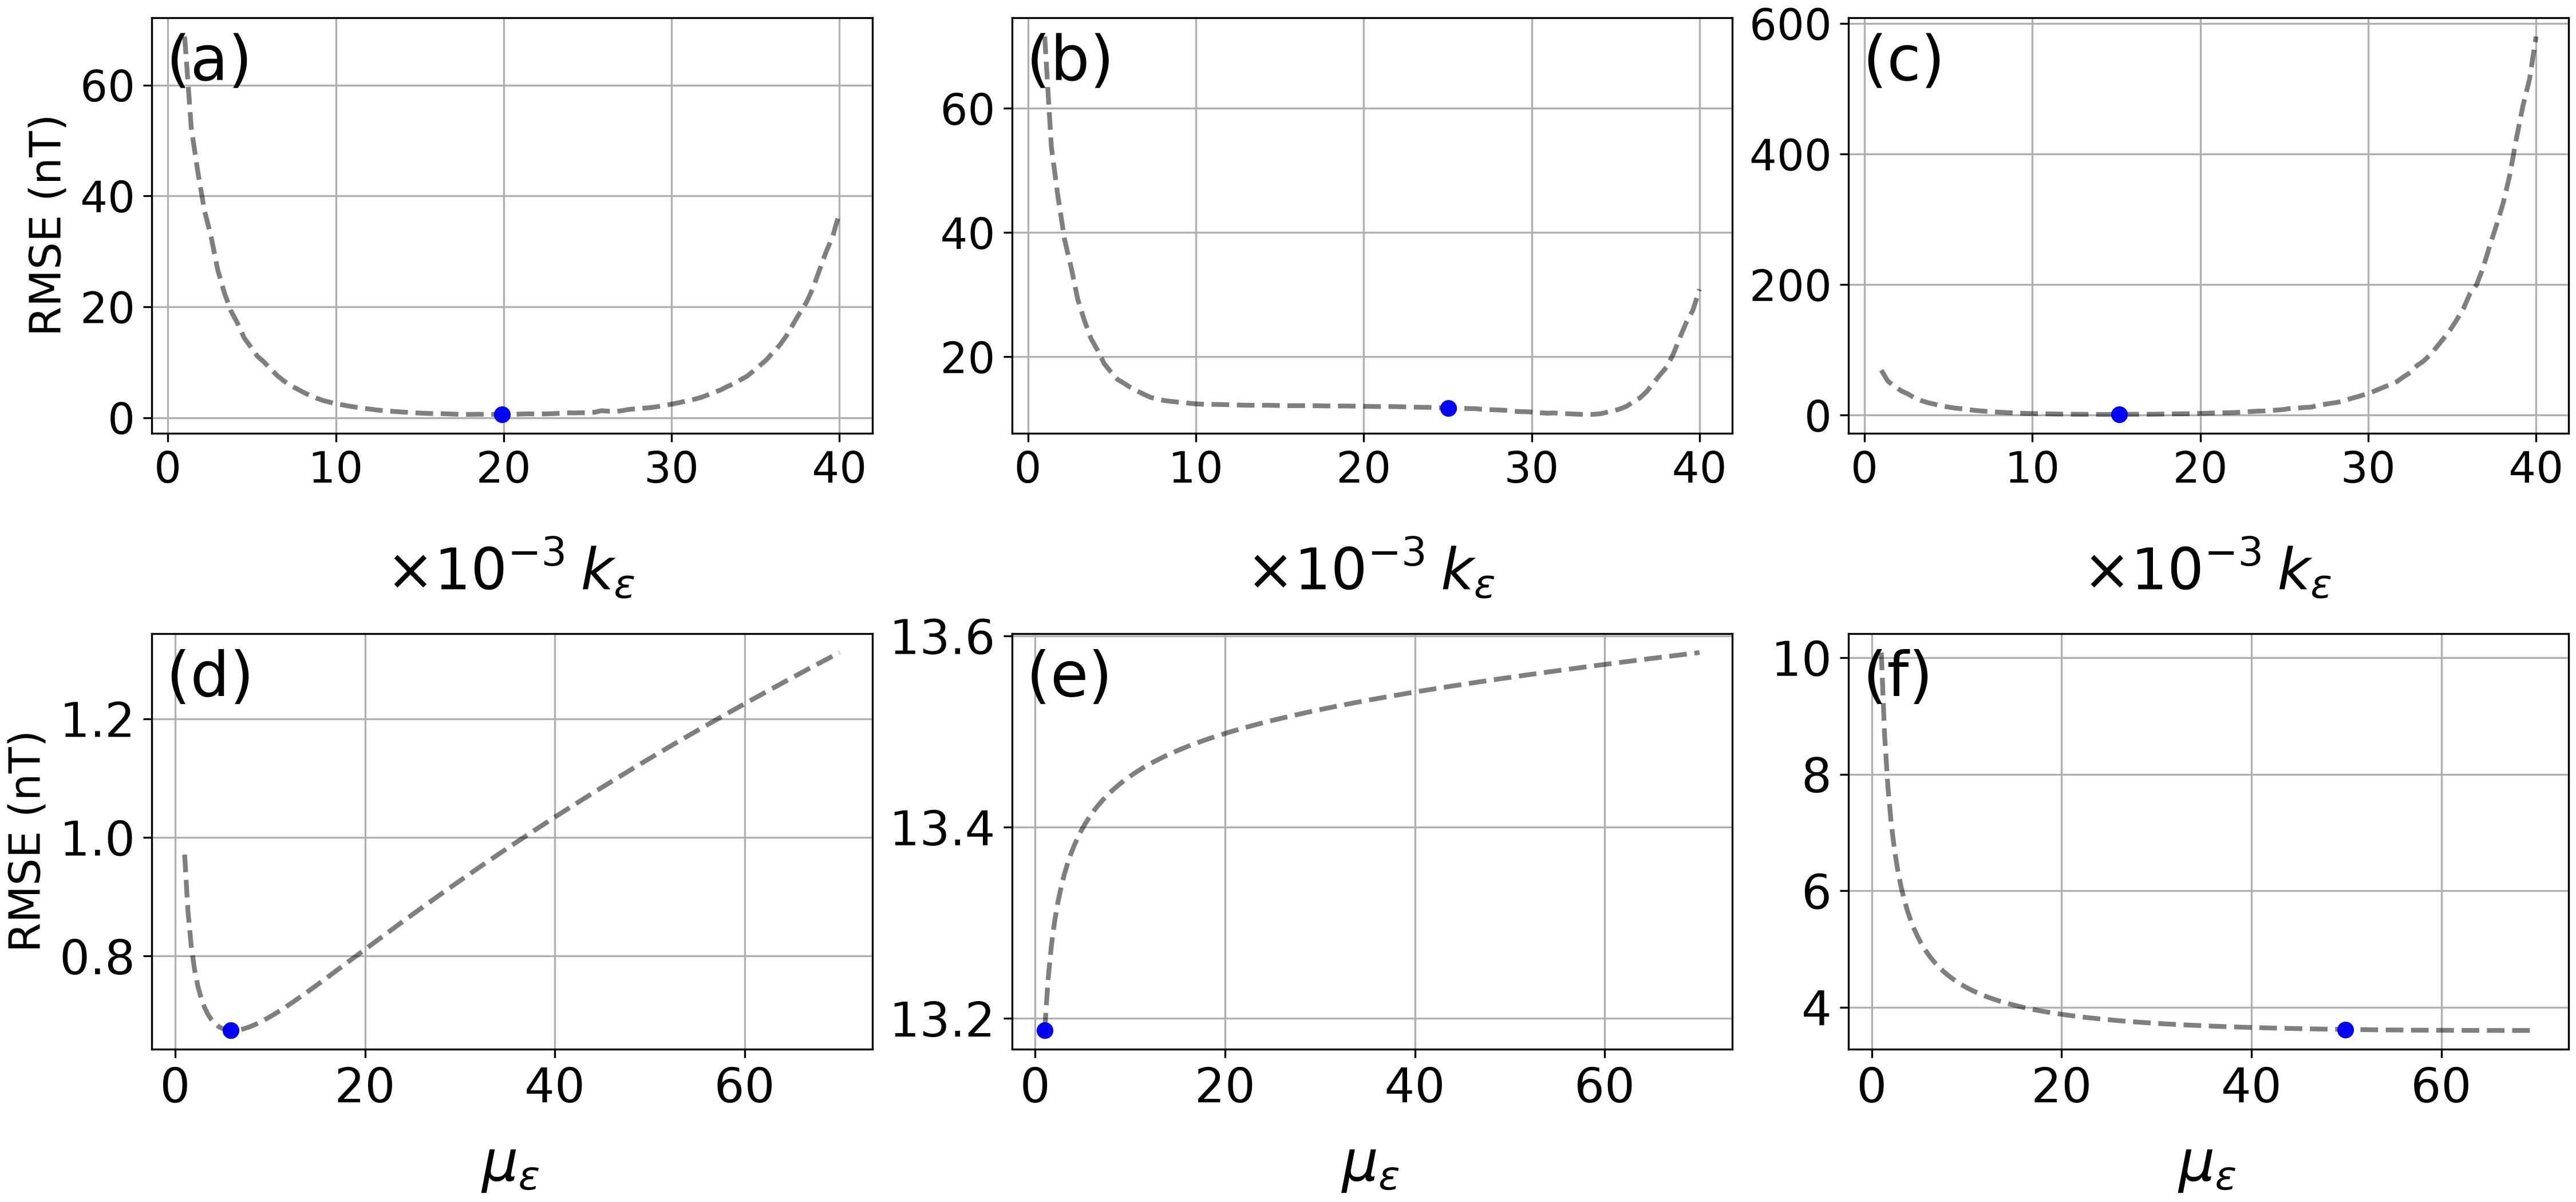
\includegraphics[width=0.8\textwidth]{Figure_S1.png}
	\caption{%
		Estimated discrete layers.
		Root Mean Square Error (RMSE) produced by discrete equivalent layers obtained by using 
		different tentative values of truncating wavenumber $k_{\varepsilon}$ 
		(equation \mainref{eq:potential-U-epsilon-Fourier-layer-1}) and regularization parameter $\mu_{\varepsilon}$
		(equation \mainref{eq:potential-U-epsilon-Fourier-layer-2}). The RMSE is defined by
		$\sqrt{\nicefrac{\| \mathbf{d}^{o} - \mathbf{d}_{\epsilon}\|^{2}_{2}}{N}}$, where 
		$\mathbf{d}^{o}$ is the approximated total-field anomaly shown in Figure \mainref{fig:Figure3}a and
		$\mathbf{d}_{\epsilon}$ is the approximated total-field anomaly predicted by the 
		corresponding equivalent layer.
		The blue dots in (a)--(f) represent the $k_{\varepsilon}$ and $\mu_{\varepsilon}$ 
		values used to obtain the discrete layers shown in Figures 
		\mainref{fig:Figure4}d--i, respectively.
	}
	\label{S-fig:FigureS1}
\end{figure}

\begin{figure}[h]
	\centering
	\noindent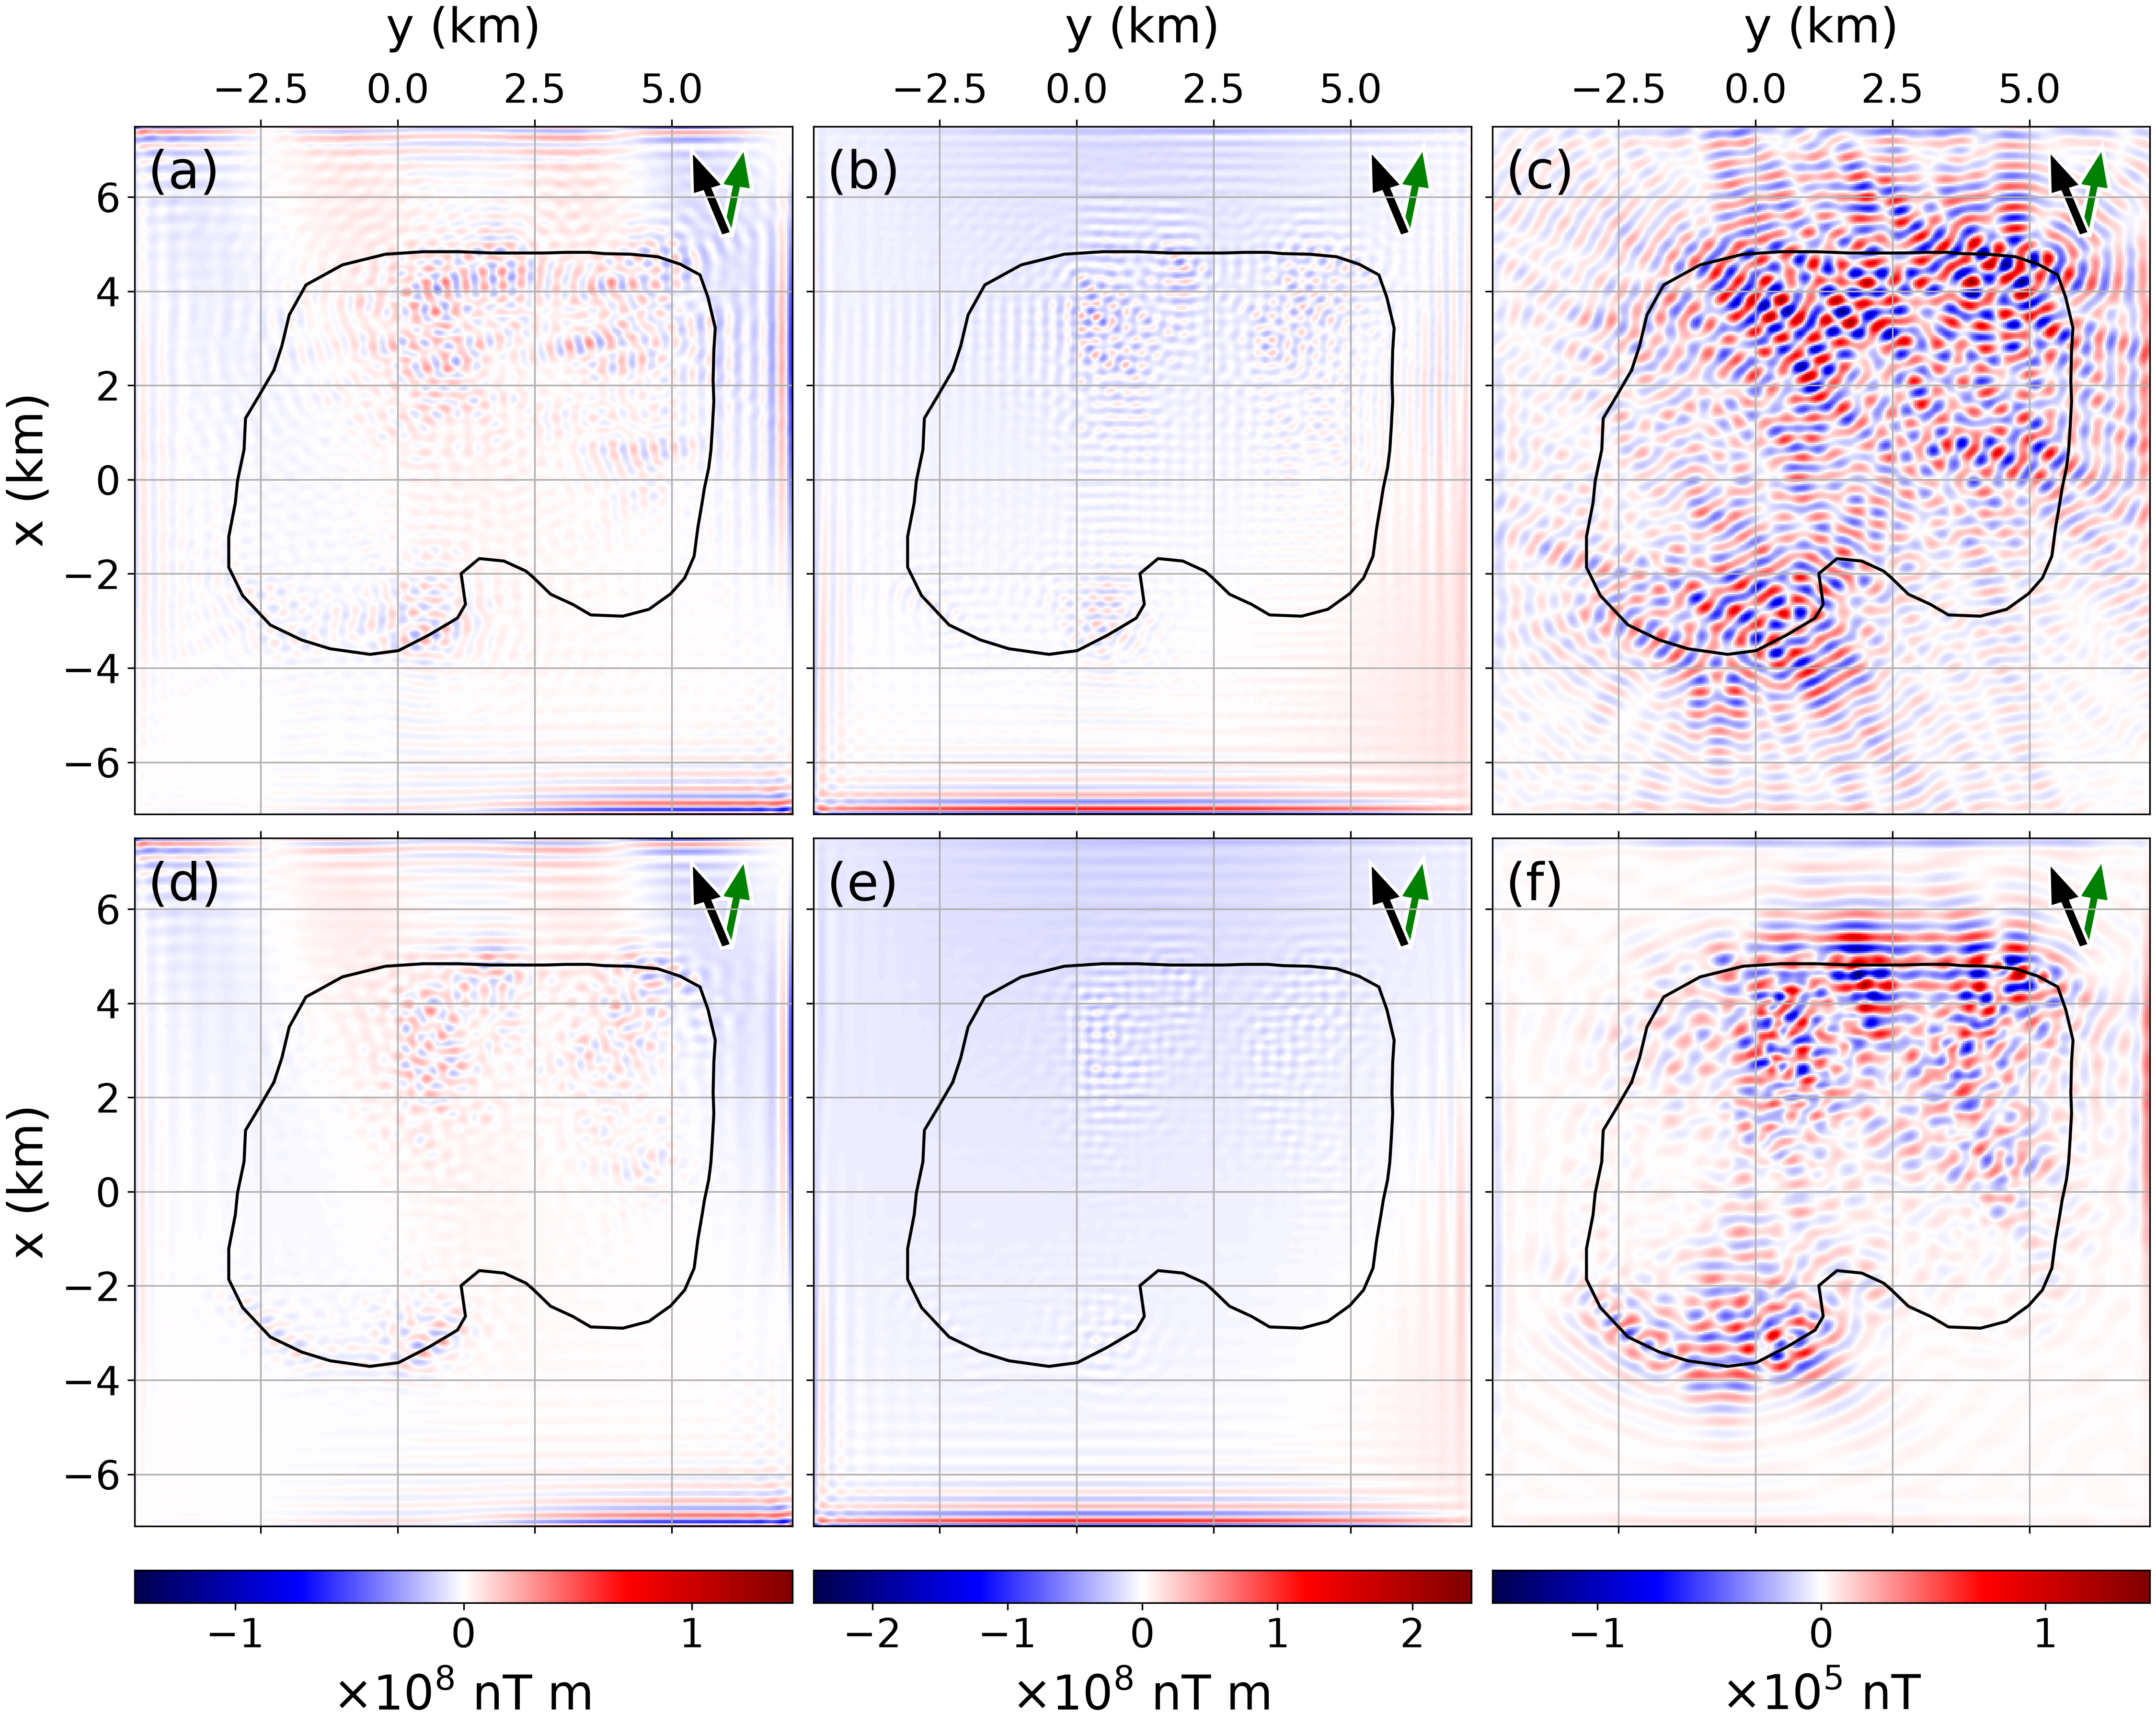
\includegraphics[width=0.8\textwidth]{Figure_S2.png}
	\caption{%
		Comparison between estimated equivalent layers shown in Figure \mainref{fig:Figure4}.
		Difference between the layers shown in Figures
		(a) \mainref{fig:Figure4}d and a; 
		(b) \mainref{fig:Figure4}e and b; 
		(c) \mainref{fig:Figure4}f and c; 
		(d) \mainref{fig:Figure4}g and a;
		(e) \mainref{fig:Figure4}h and b;
		(f) \mainref{fig:Figure4}i and c.
		The black line represents the projection of the model on the $xy$ plane.
		The green and black arrows represent, respectively, the projections of the constant 
		main field and synthetic source (Figure \mainref{fig:Figure2}) magnetization directions onto the plane $xy$.
	}
	\label{S-fig:FigureS2}
\end{figure}

\begin{table}[h]
	\caption{%
		Pearson correlation coefficient $r$ between the discrete layers shown in Figure \mainref{fig:Figure4}. 
	}
	\begin{tabular}{ccc}
		\toprule%
		{\small \textbf{Figure of layer a }} & 
		{\small \textbf{Figure of layer b}} & 
		{\small \textbf{r}} \\
		\midrule%
		\mainref{fig:Figure4}d & \mainref{fig:Figure4}a & $0.99$ \\
		\mainref{fig:Figure4}e & \mainref{fig:Figure4}b & $0.96$ \\
		\mainref{fig:Figure4}f & \mainref{fig:Figure4}c & $0.96$ \\
		\mainref{fig:Figure4}g & \mainref{fig:Figure4}a & $0.99$ \\
		\mainref{fig:Figure4}h & \mainref{fig:Figure4}b & $0.96$ \\
		\mainref{fig:Figure4}i & \mainref{fig:Figure4}c & $0.98$ \\
		\botrule%
	\end{tabular}
	\label{S-tbl:TableS2}
\end{table}

\begin{figure}[h]
	\centering
	\noindent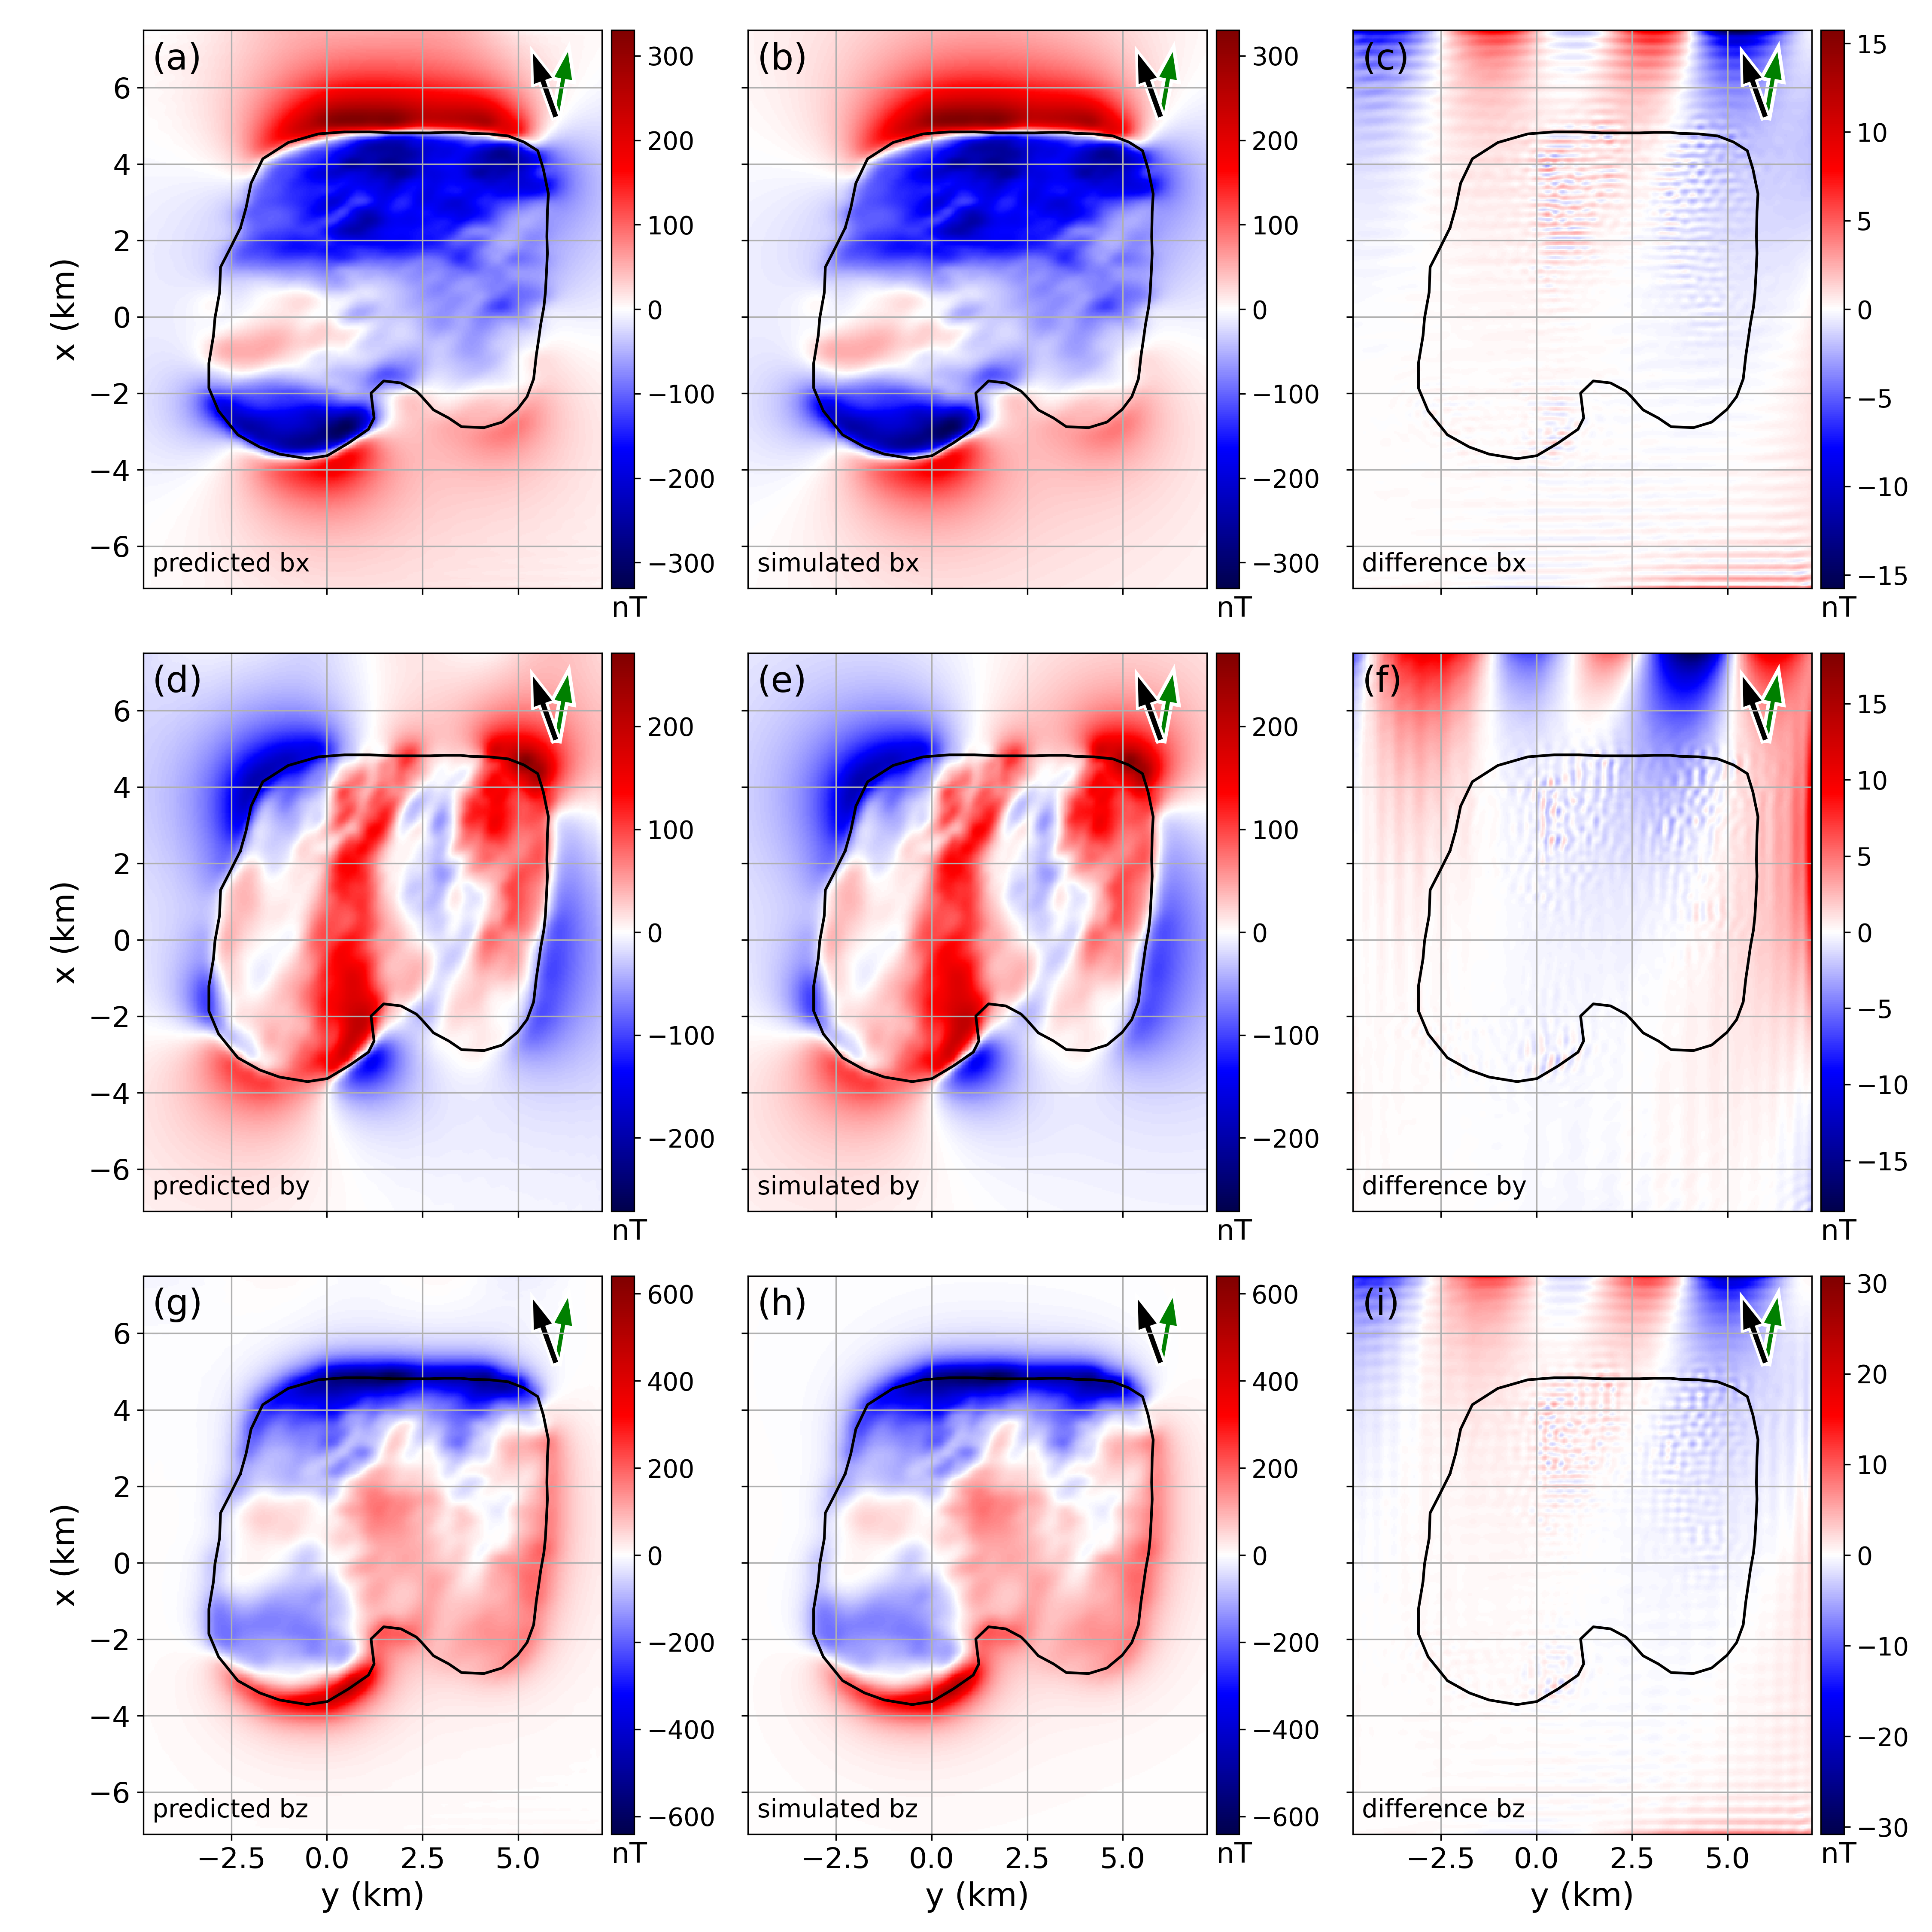
\includegraphics[width=0.8\textwidth]{Figure_S3.png}
	\caption{%
		Comparison between the simulated fields and those predicted by the estimated equivalent layer shown in Figure \mainref{fig:Figure4}a.
	}
	\label{S-fig:FigureS3}
\end{figure}

\begin{figure}[h]
	\centering
	\noindent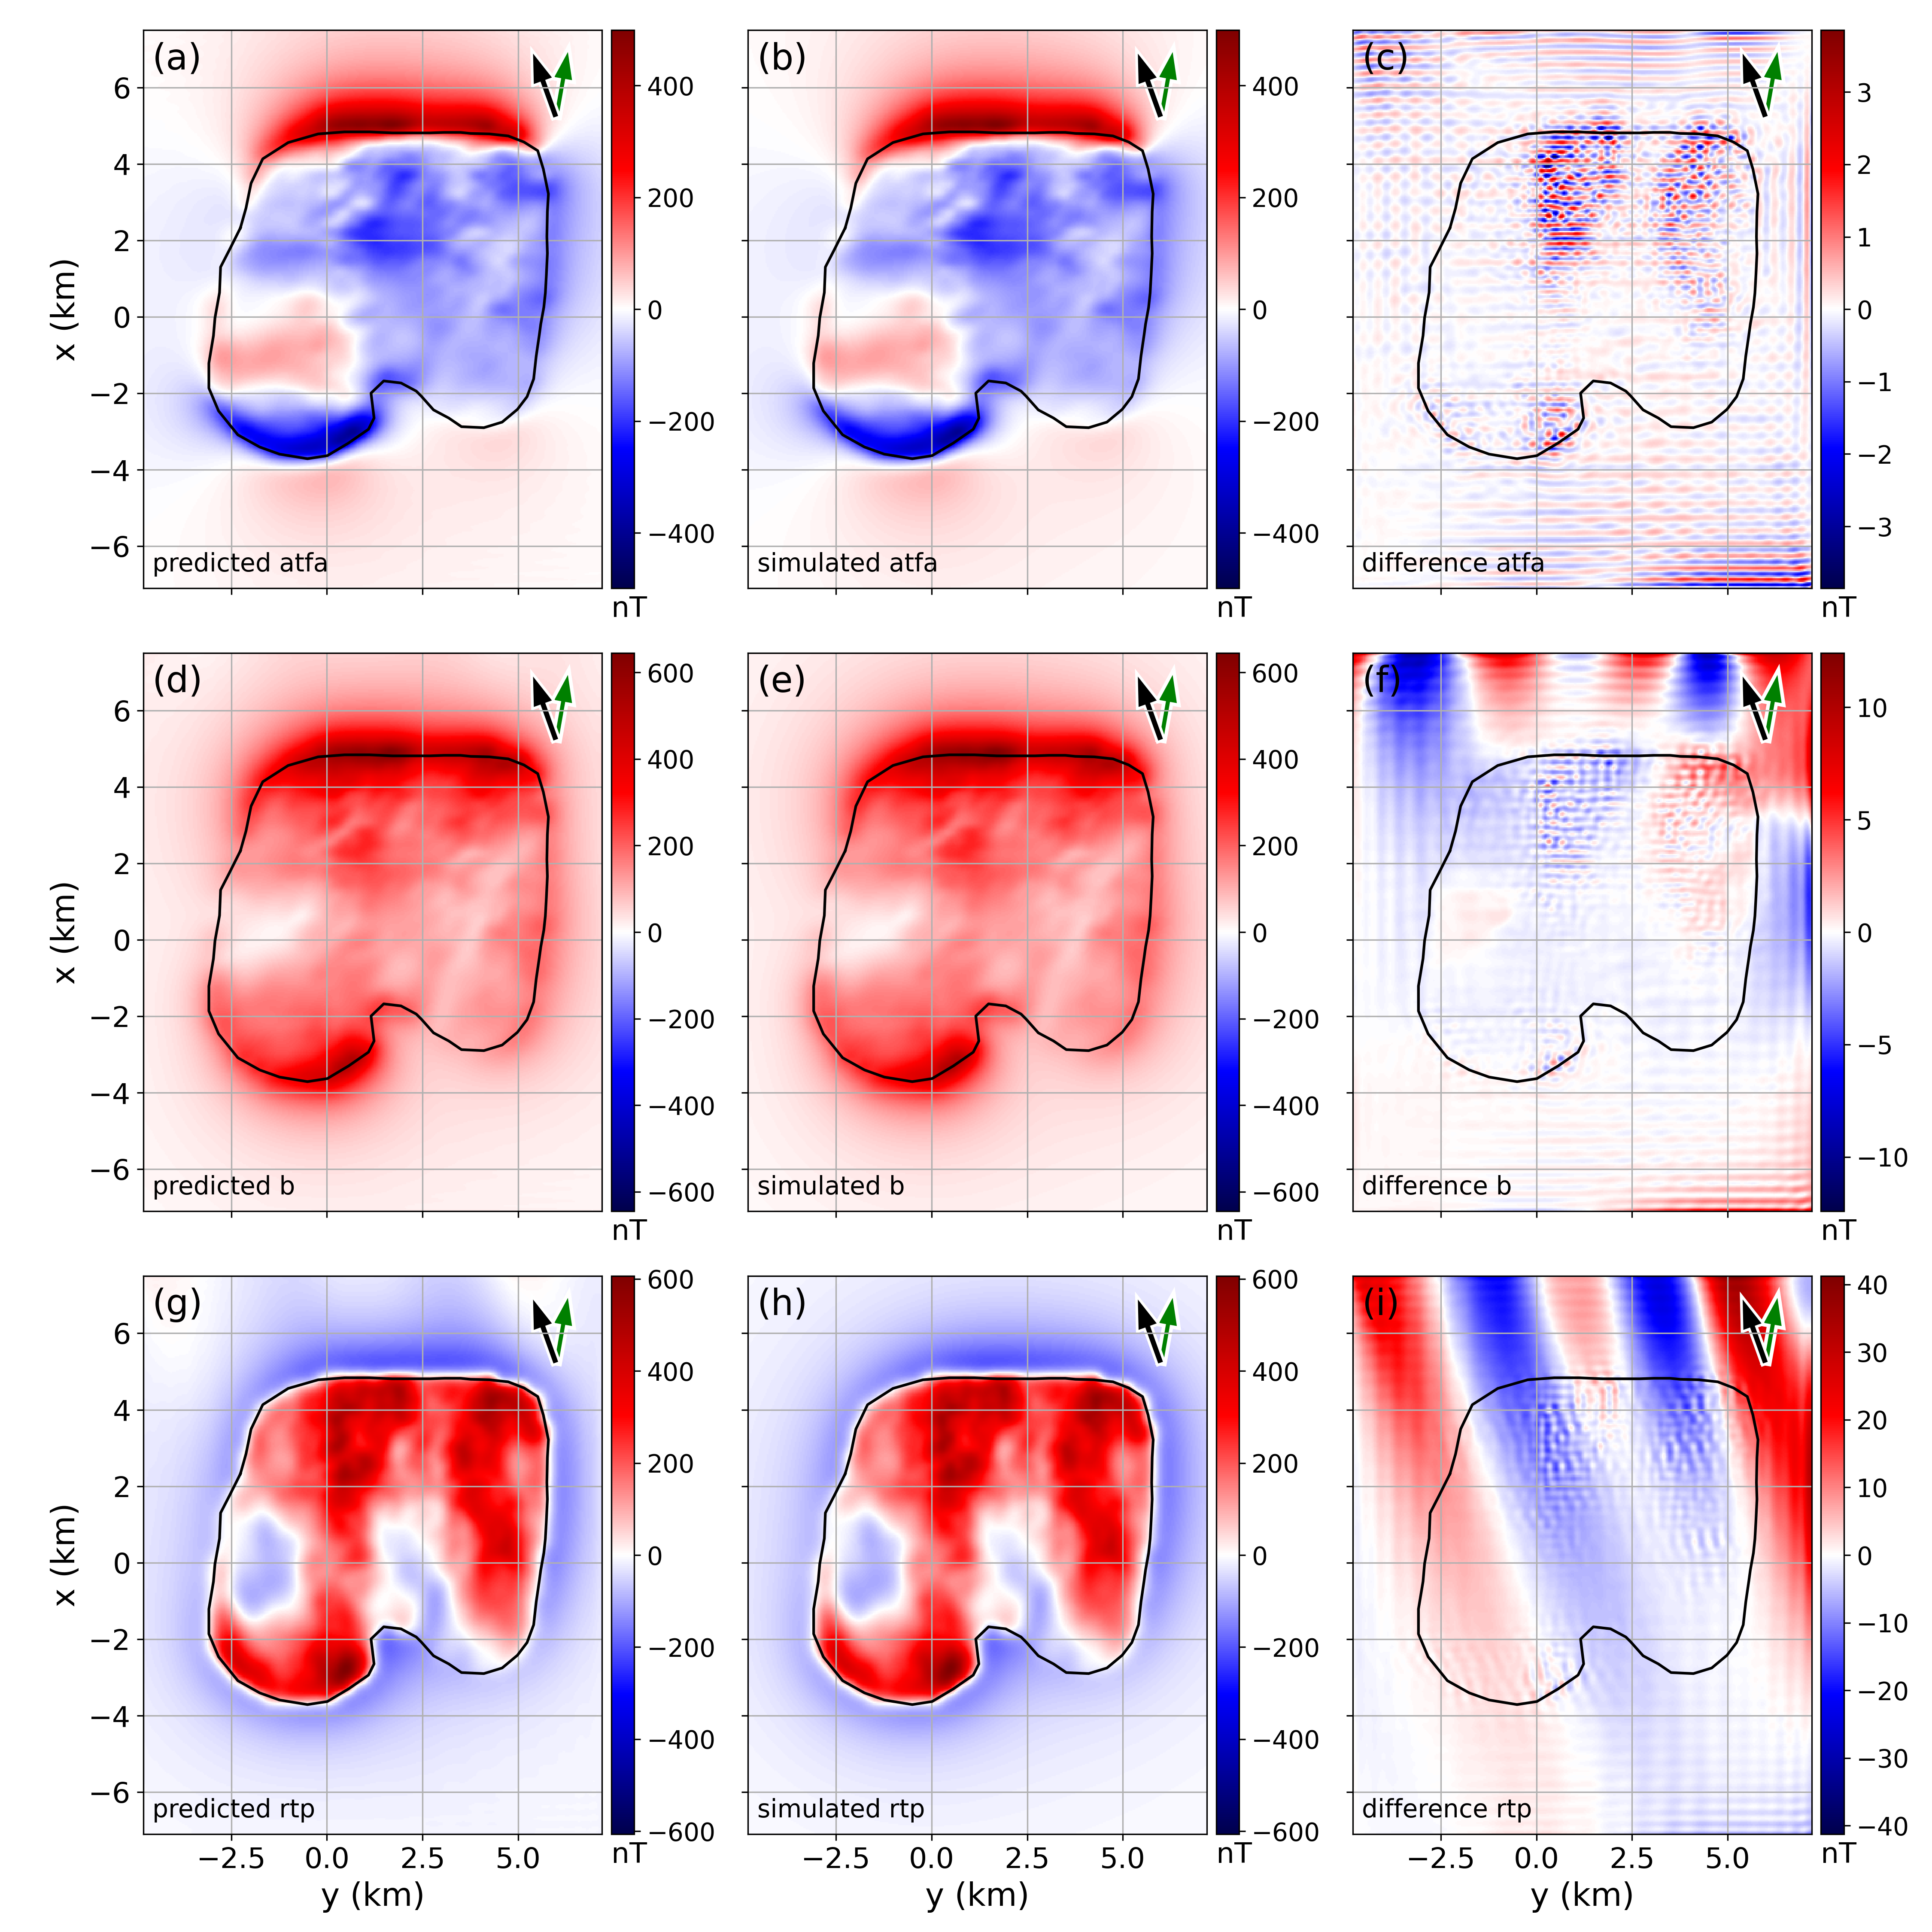
\includegraphics[width=0.8\textwidth]{Figure_S4.png}
	\caption{%
		Comparison between the simulated fields and those predicted by the estimated equivalent layer shown in Figure \mainref{fig:Figure4}a.
	}
	\label{S-fig:FigureS4}
\end{figure}

\begin{figure}[h]
	\centering
	\noindent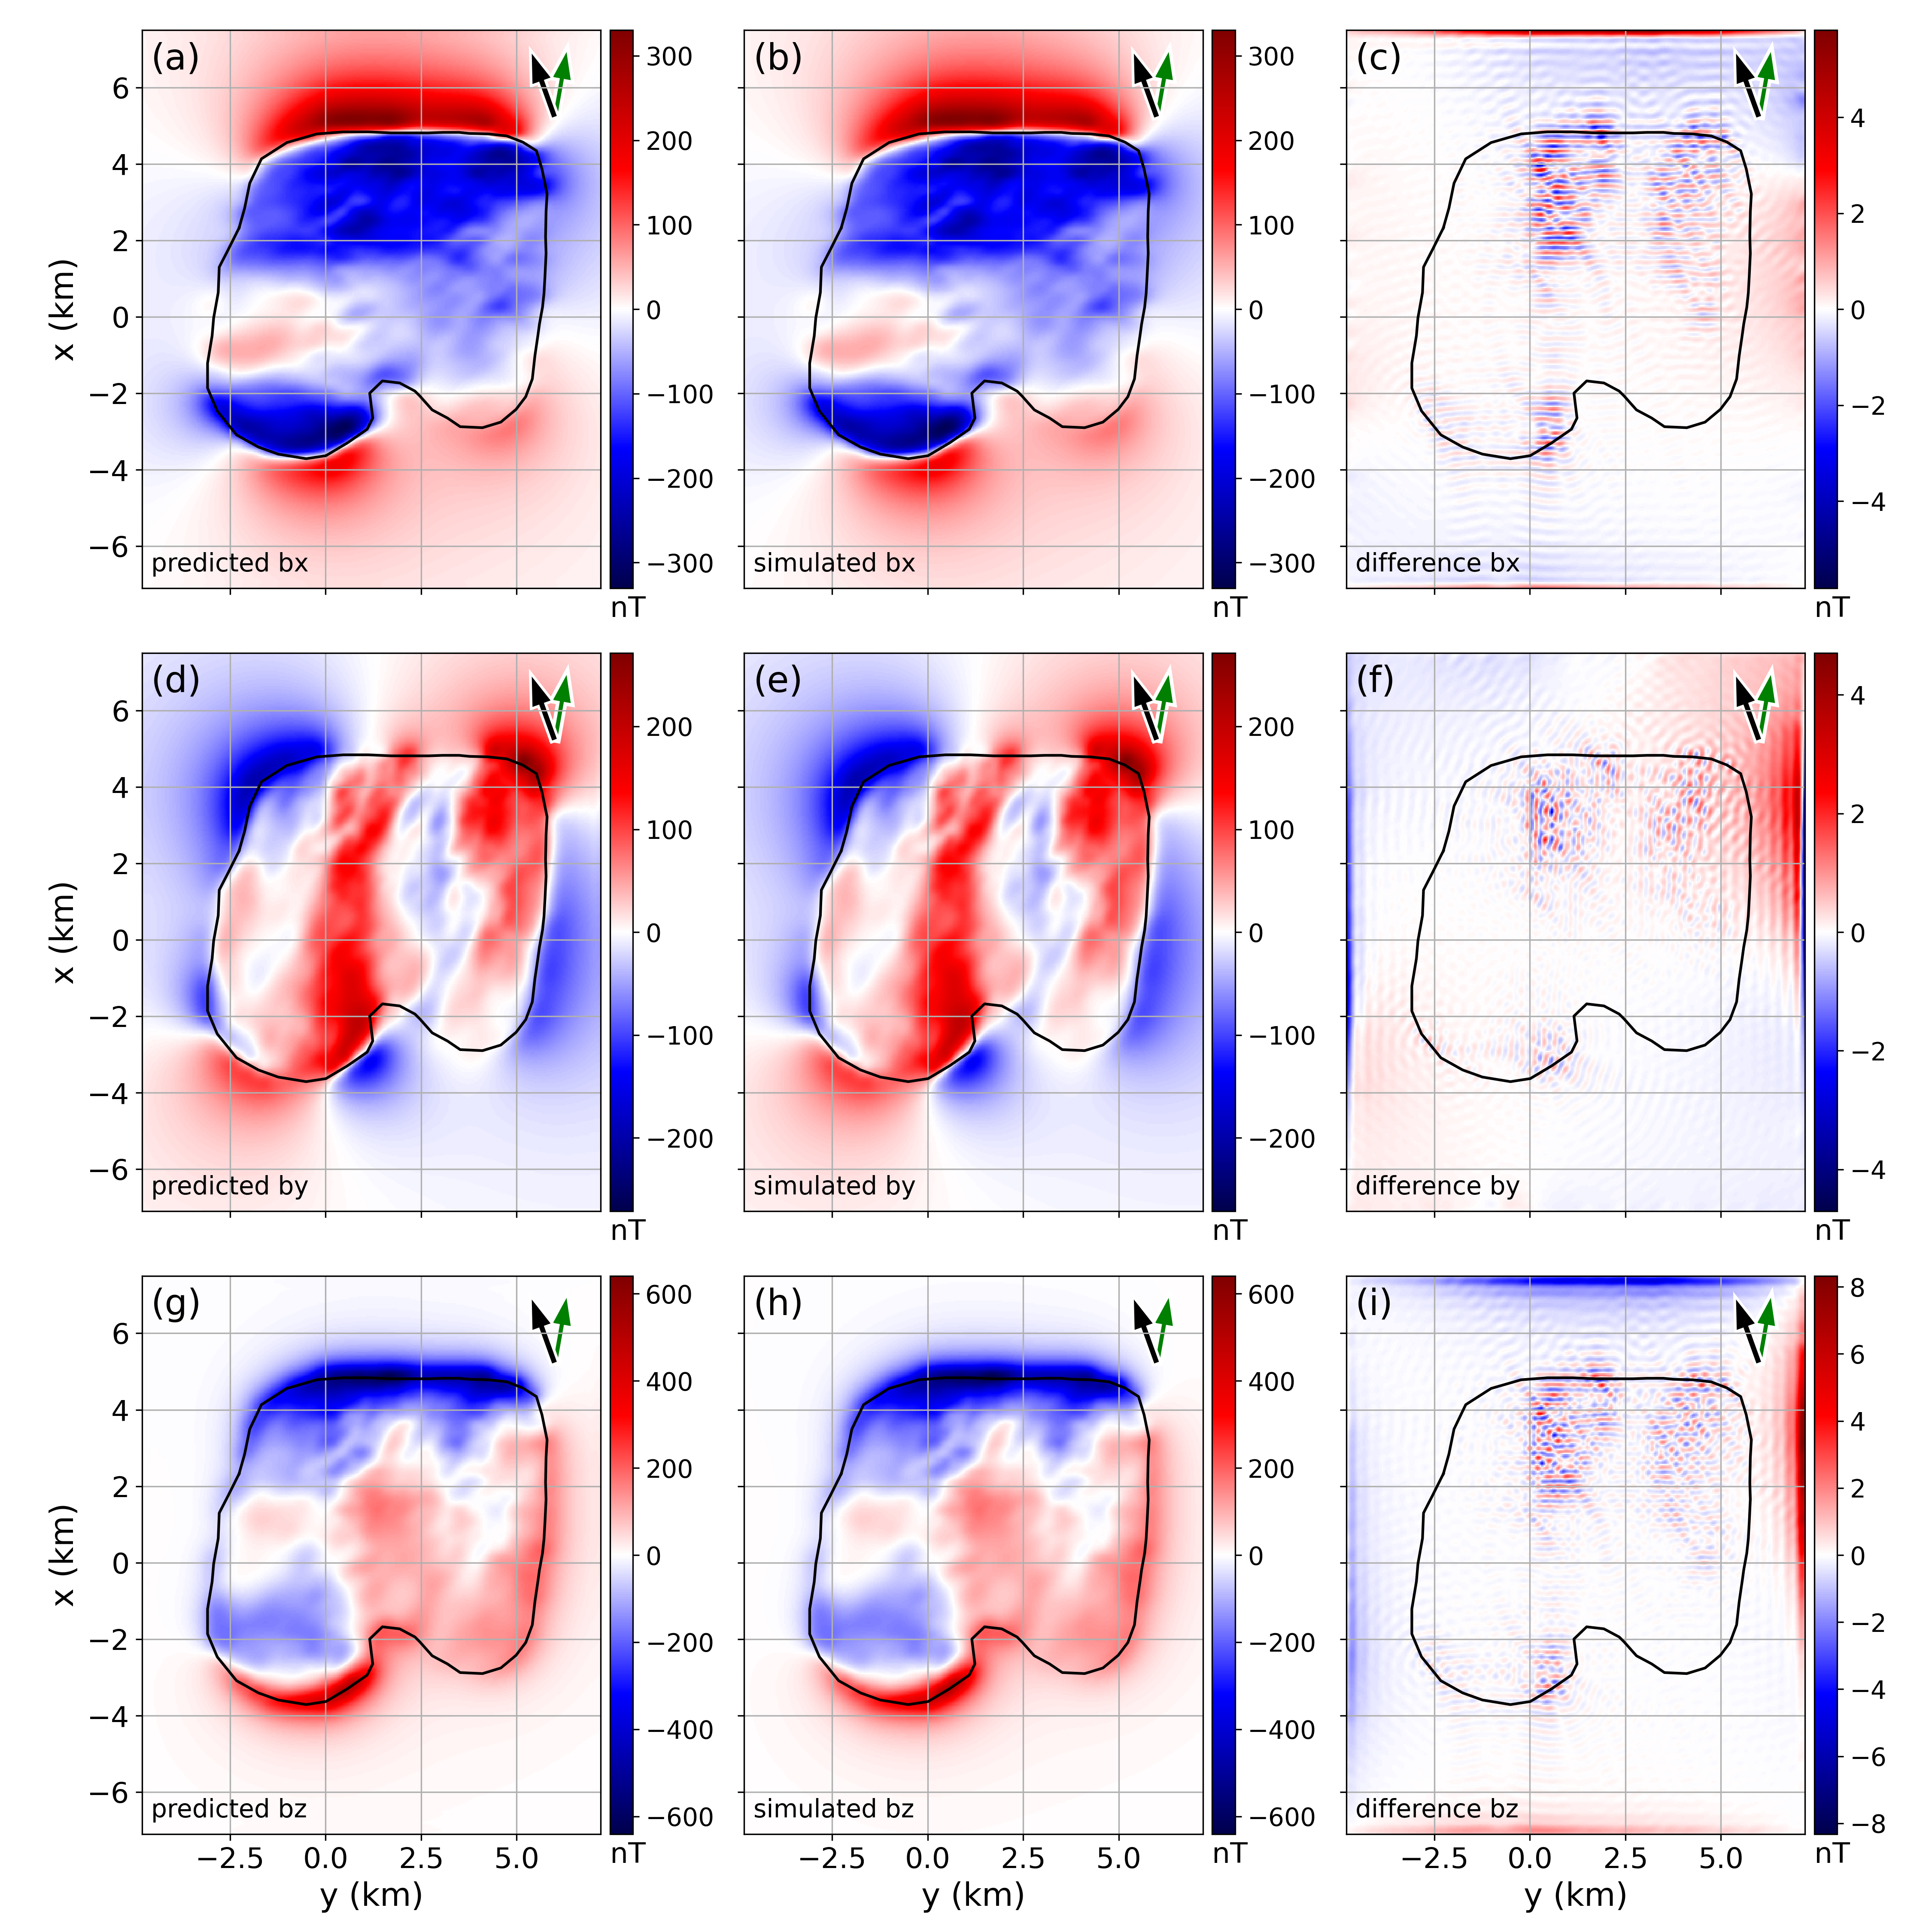
\includegraphics[width=0.8\textwidth]{Figure_S5.png}
	\caption{%
		Comparison between the simulated fields and those predicted by the estimated equivalent layer shown in Figure \mainref{fig:Figure4}d.
	}
	\label{S-fig:FigureS5}
\end{figure}

\begin{figure}[h]
	\centering
	\noindent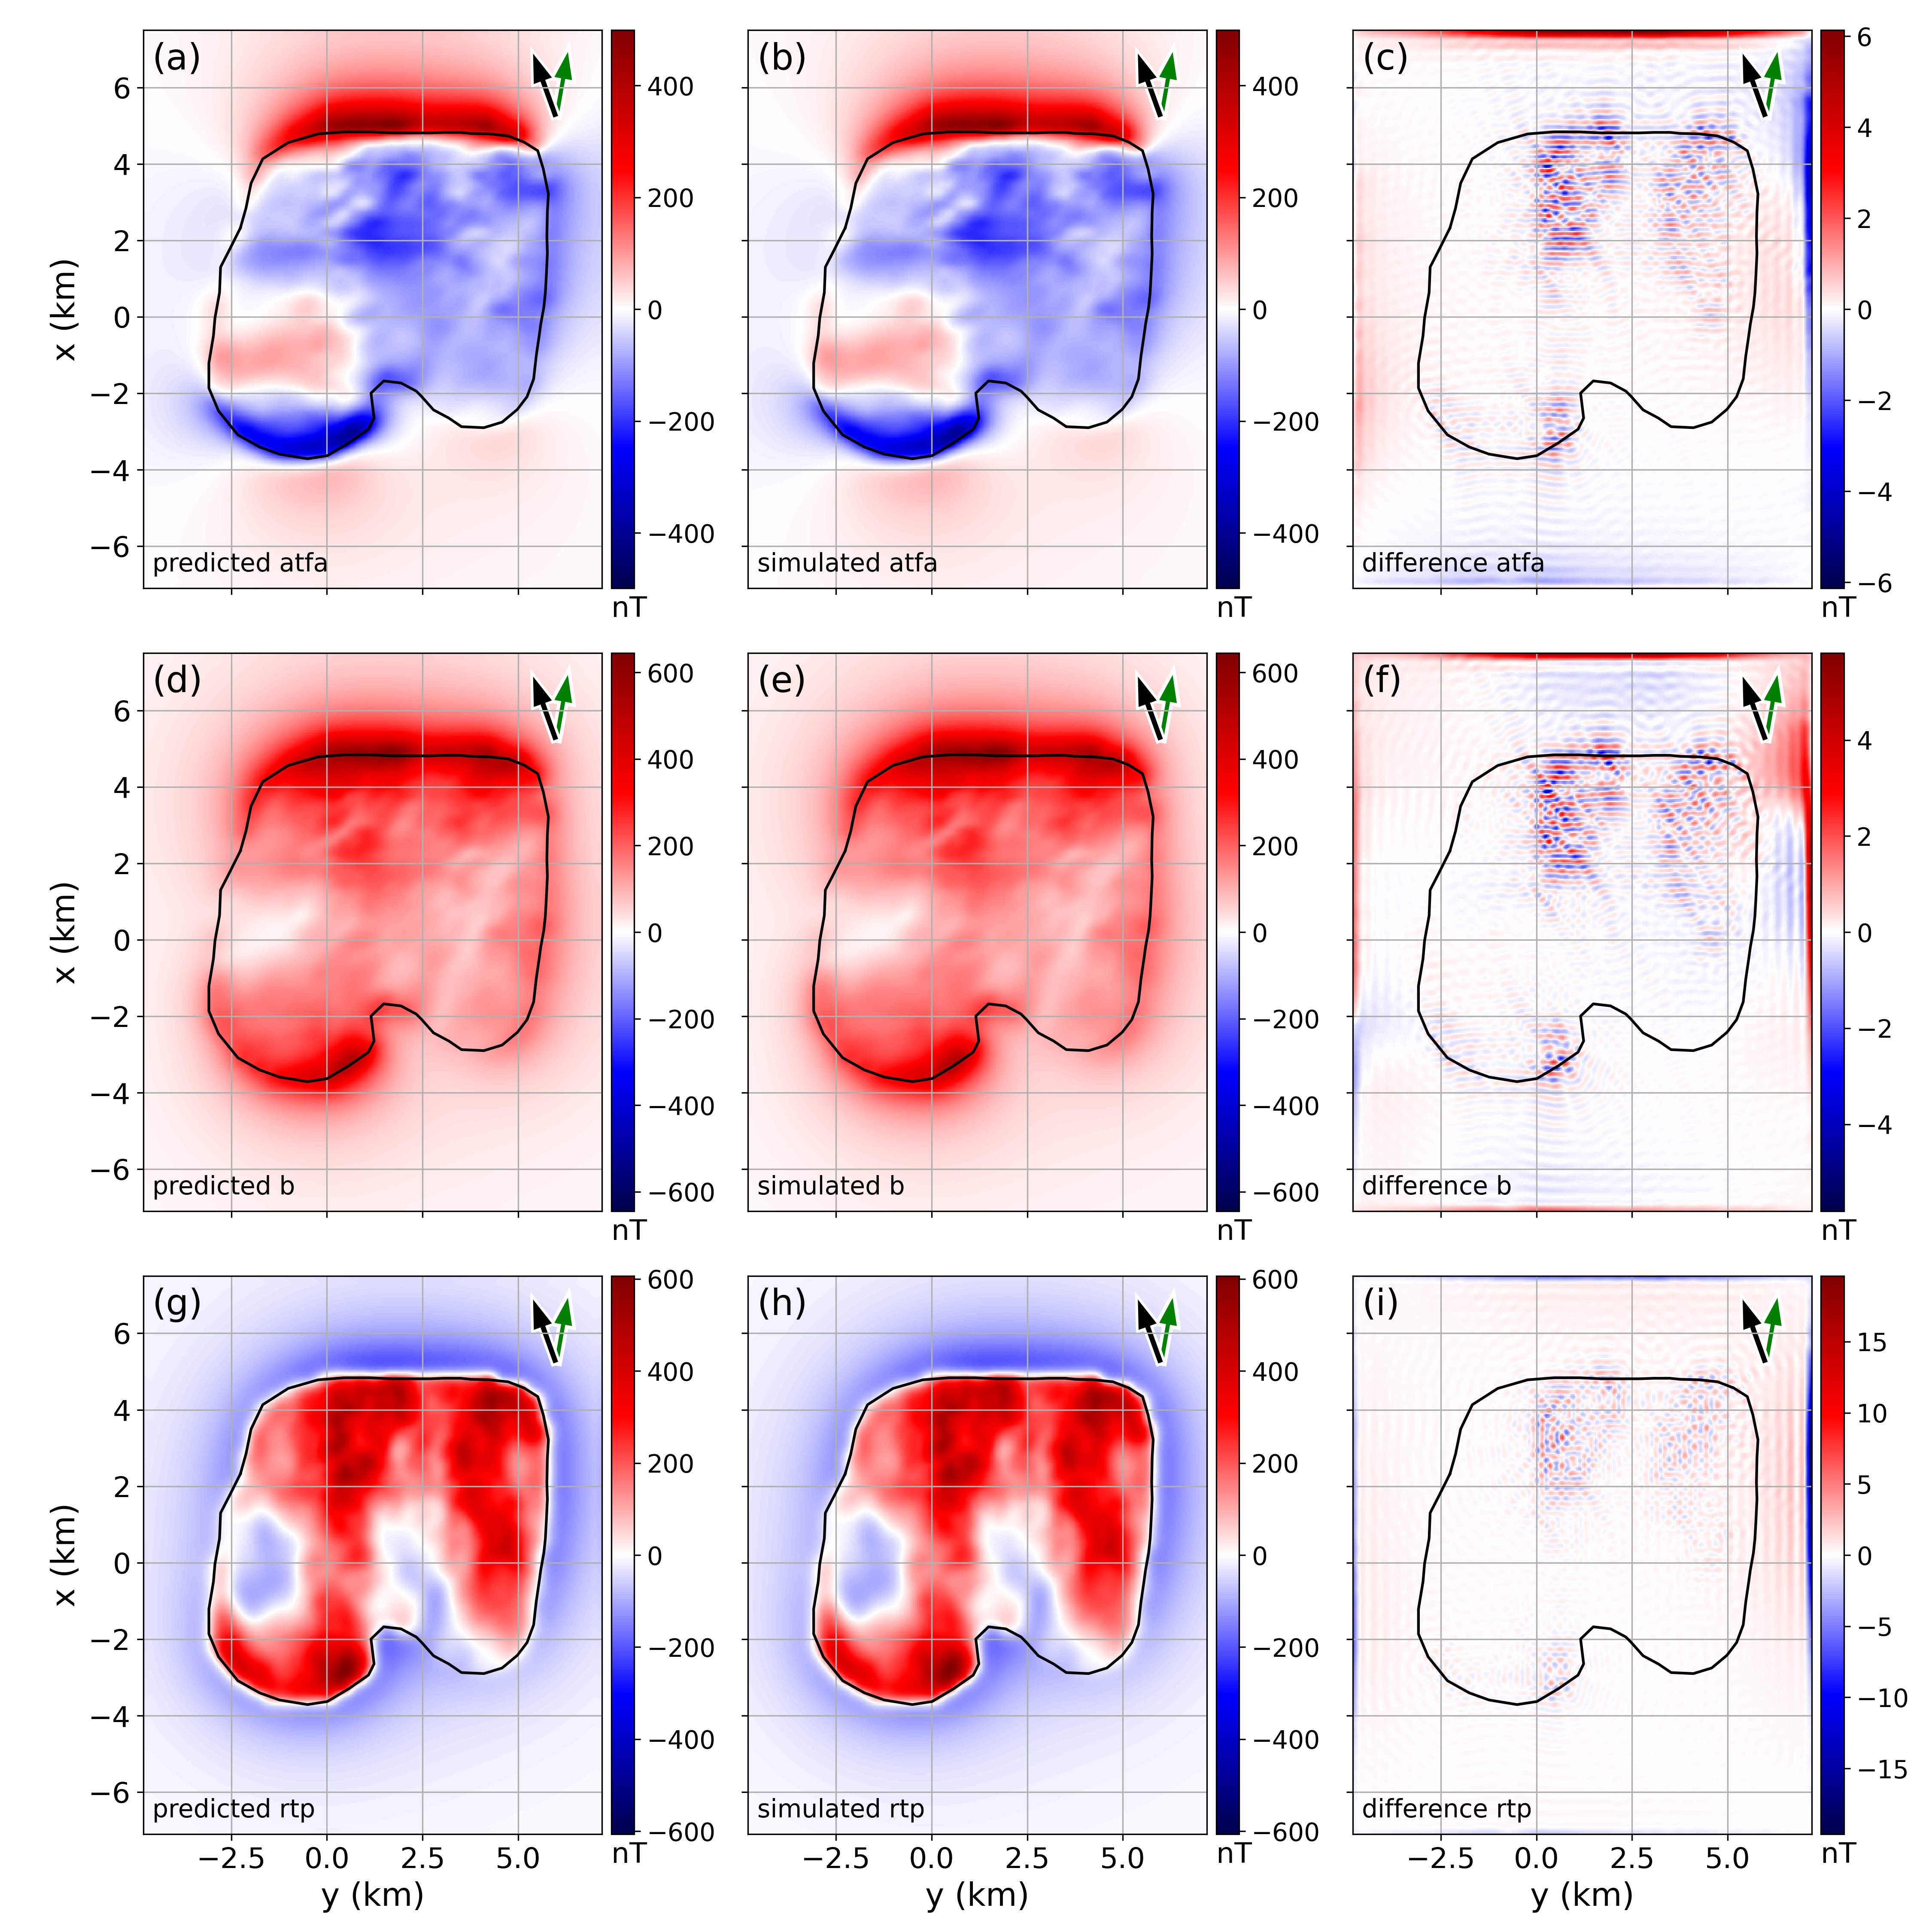
\includegraphics[width=0.8\textwidth]{Figure_S6.png}
	\caption{%
		Comparison between the simulated fields and those predicted by the estimated equivalent layer shown in Figure \mainref{fig:Figure4}d.
	}
	\label{S-fig:FigureS6}
\end{figure}

\begin{figure}[h]
	\centering
	\noindent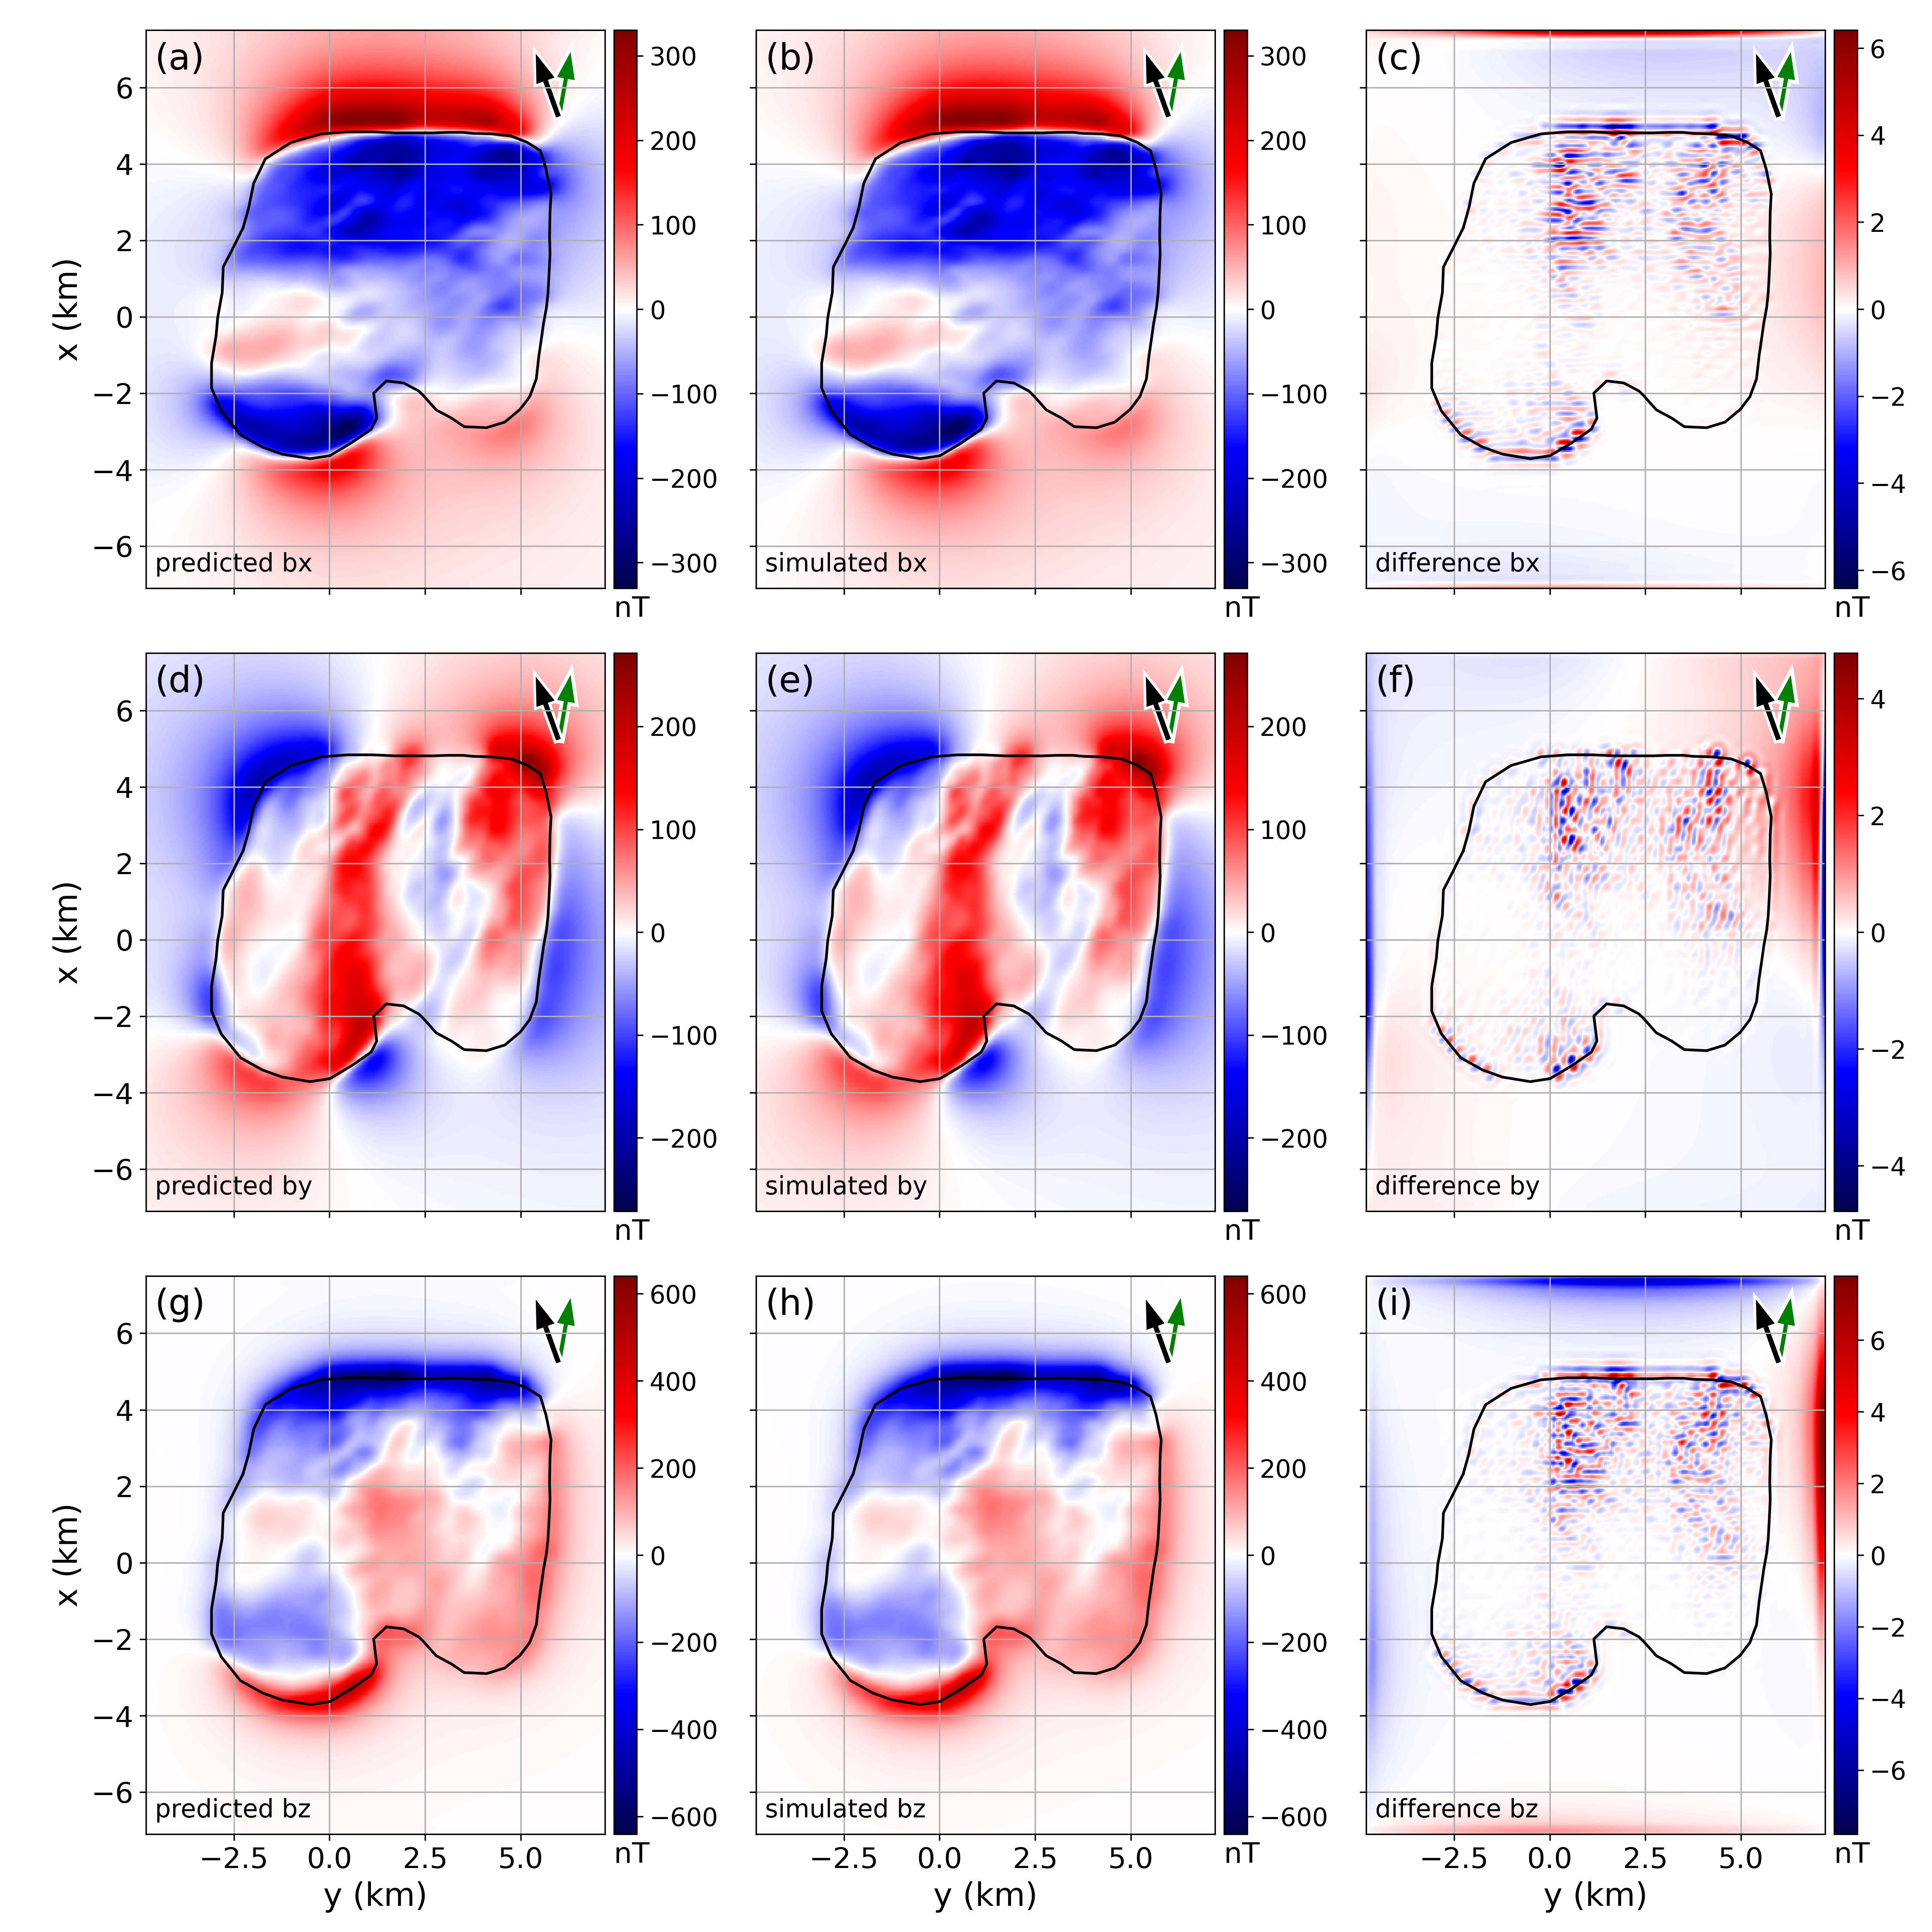
\includegraphics[width=0.8\textwidth]{Figure_S7.png}
	\caption{%
		Comparison between the simulated fields and those predicted by the estimated equivalent layer shown in Figure \mainref{fig:Figure4}g.
	}
	\label{S-fig:FigureS7}
\end{figure}

\begin{figure}[h]
	\centering
	\noindent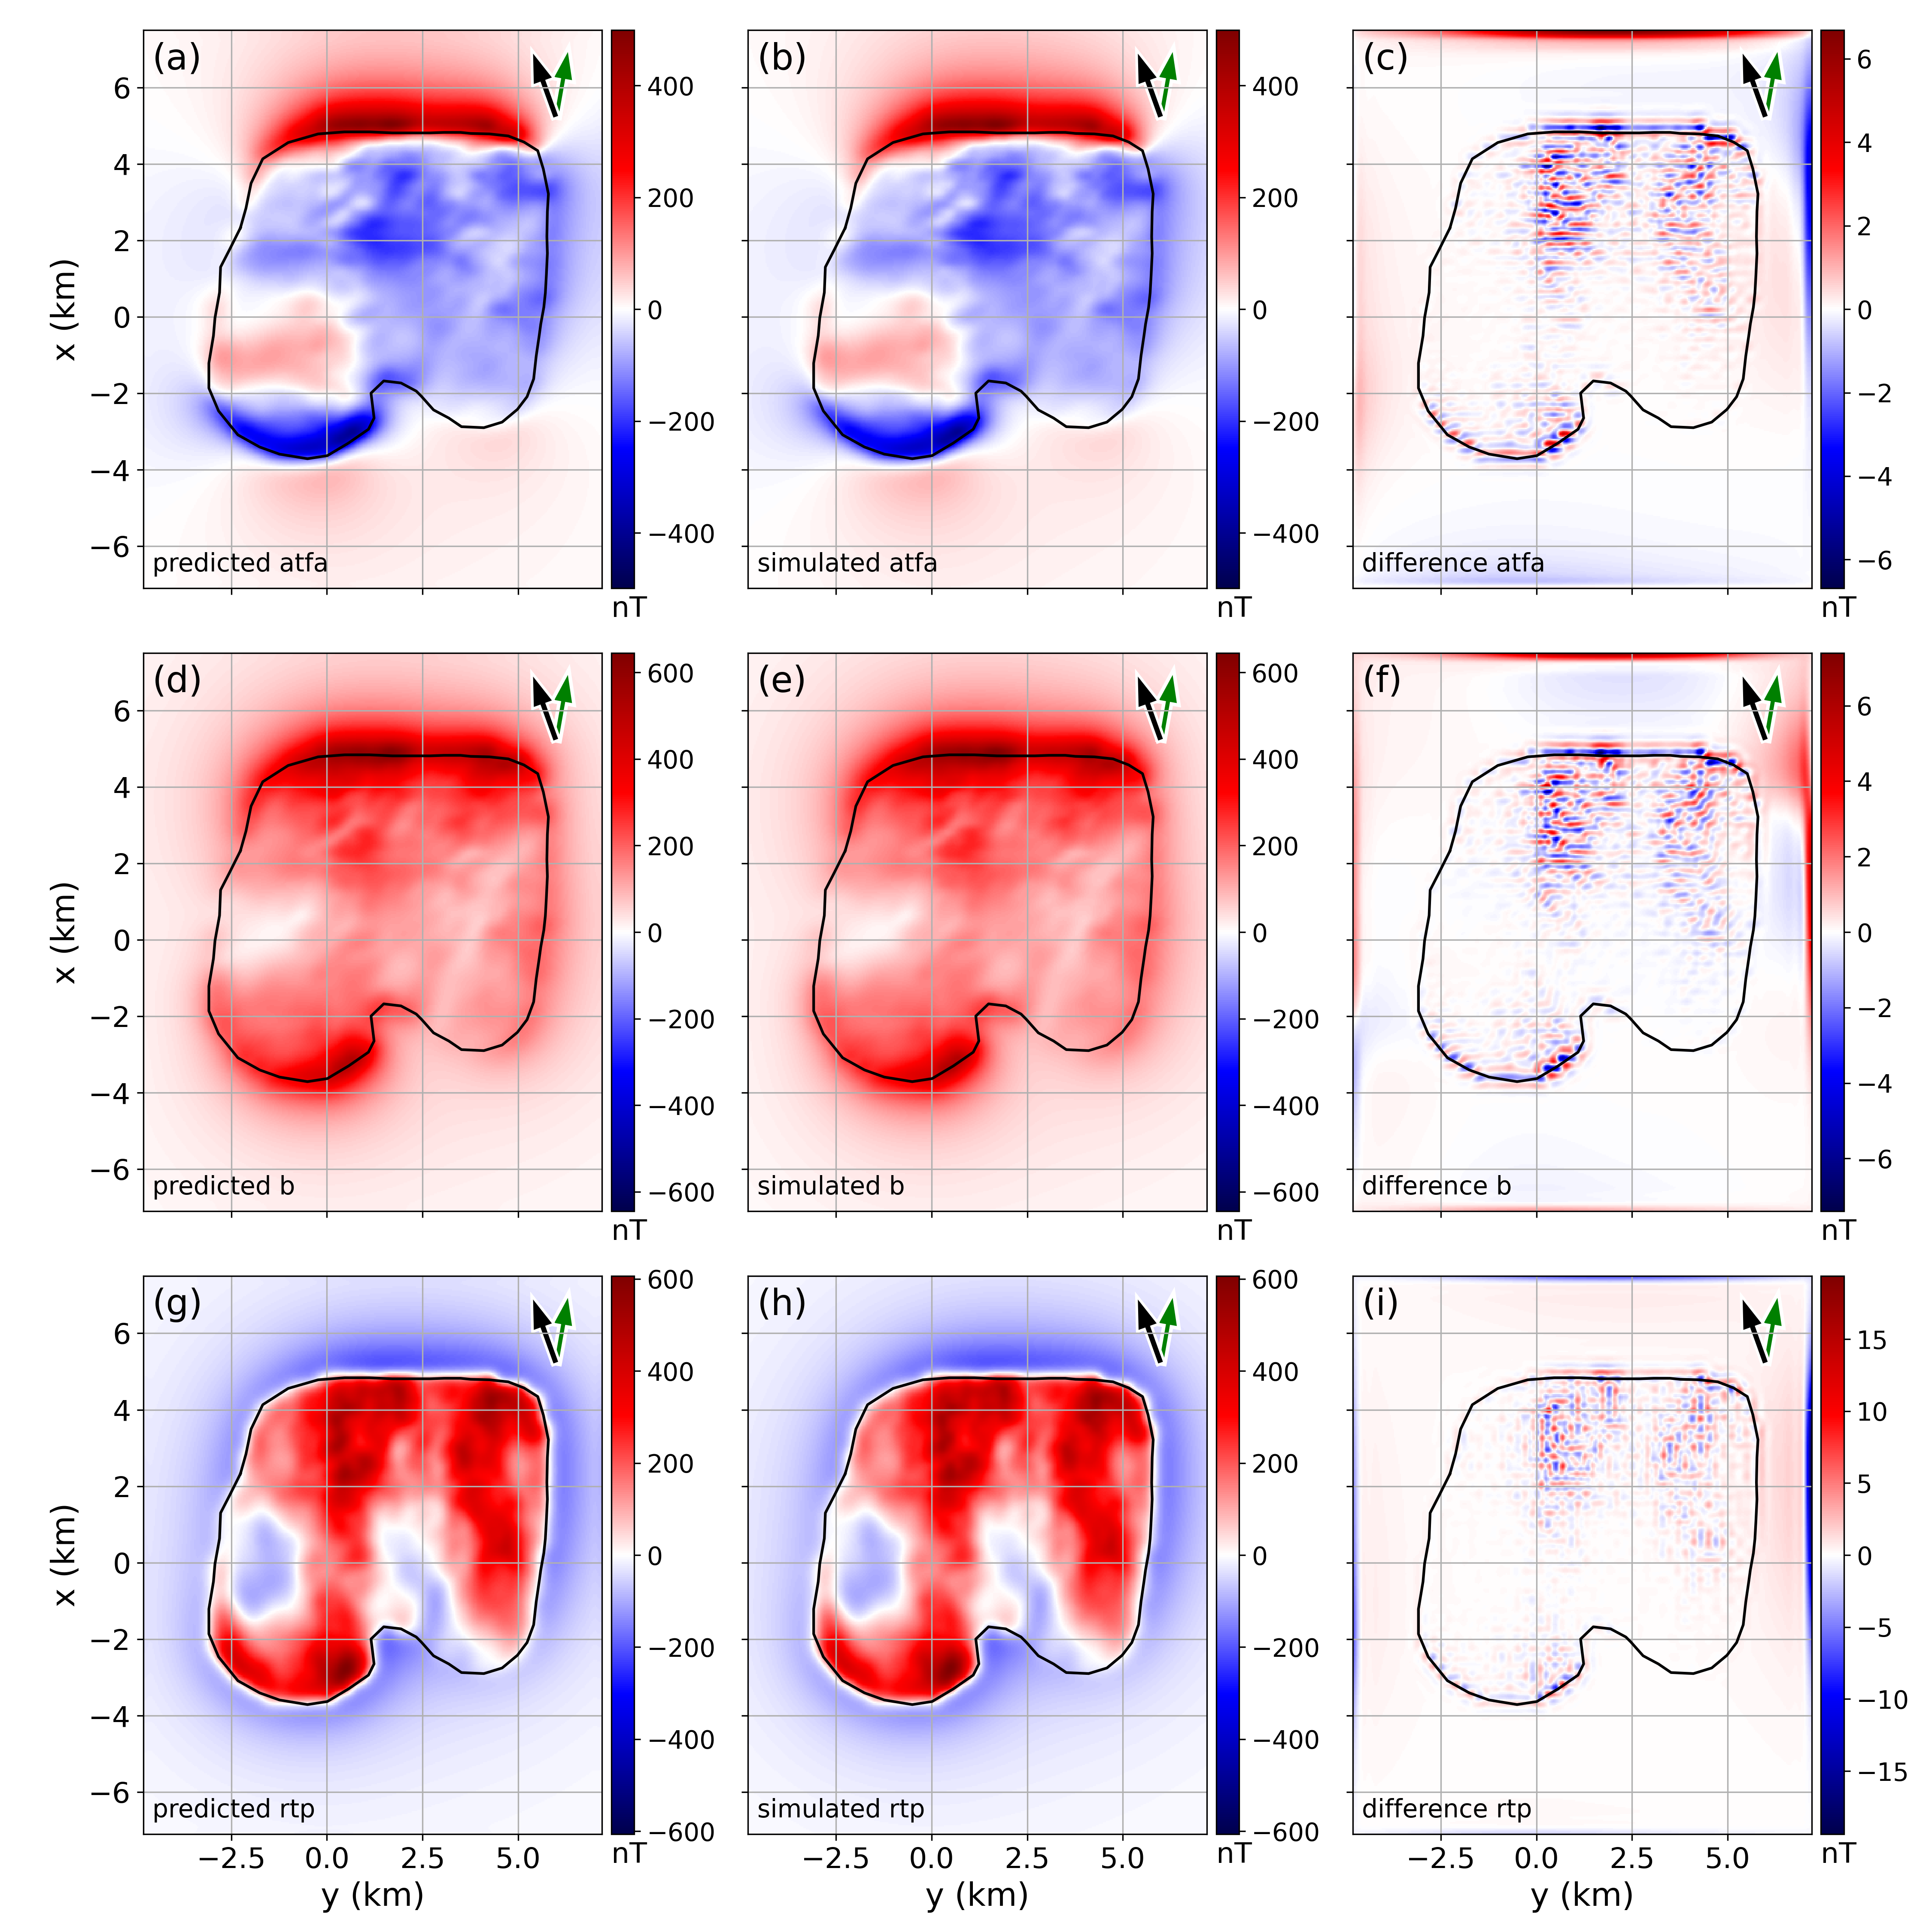
\includegraphics[width=0.8\textwidth]{Figure_S8.png}
	\caption{%
		Comparison between the simulated fields and those predicted by the estimated equivalent layer shown in Figure \mainref{fig:Figure4}g.
	}
	\label{S-fig:FigureS8}
\end{figure}

\begin{figure}[h]
	\centering
	\noindent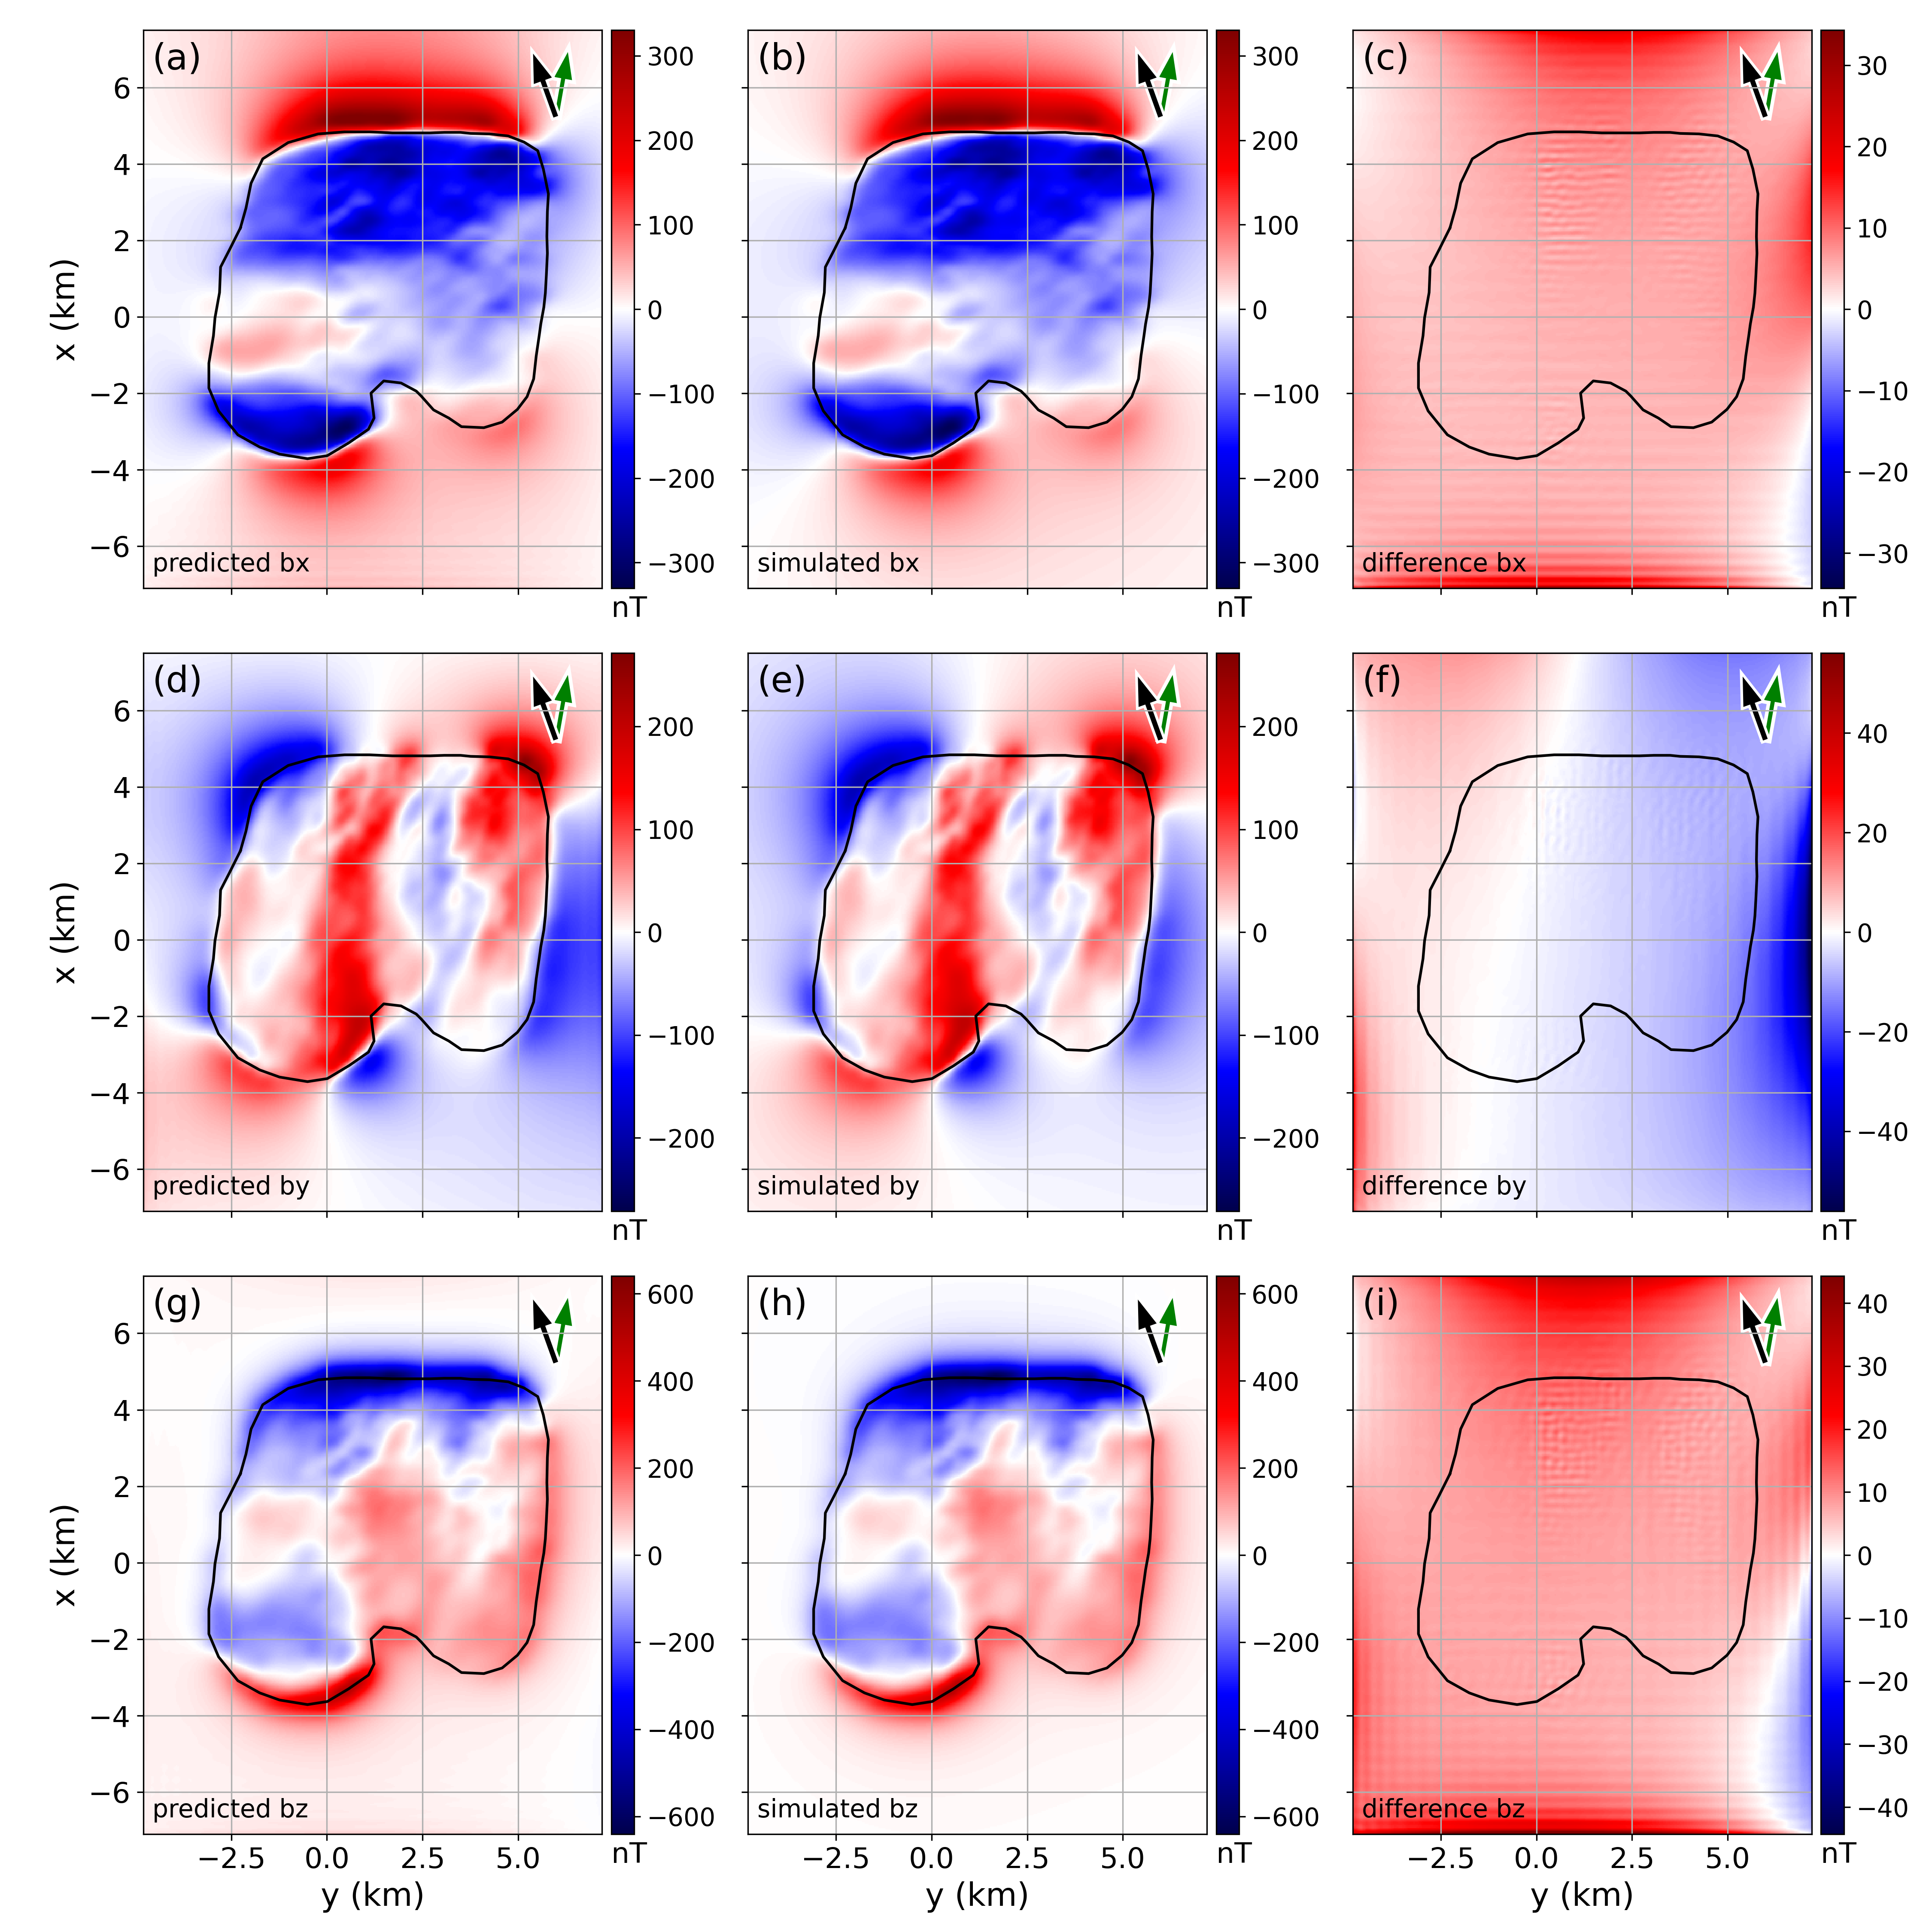
\includegraphics[width=0.8\textwidth]{Figure_S9.png}
	\caption{%
		Comparison between the simulated fields and those predicted by the estimated equivalent layer shown in Figure \mainref{fig:Figure4}b.
	}
	\label{S-fig:FigureS9}
\end{figure}

\begin{figure}[h]
	\centering
	\noindent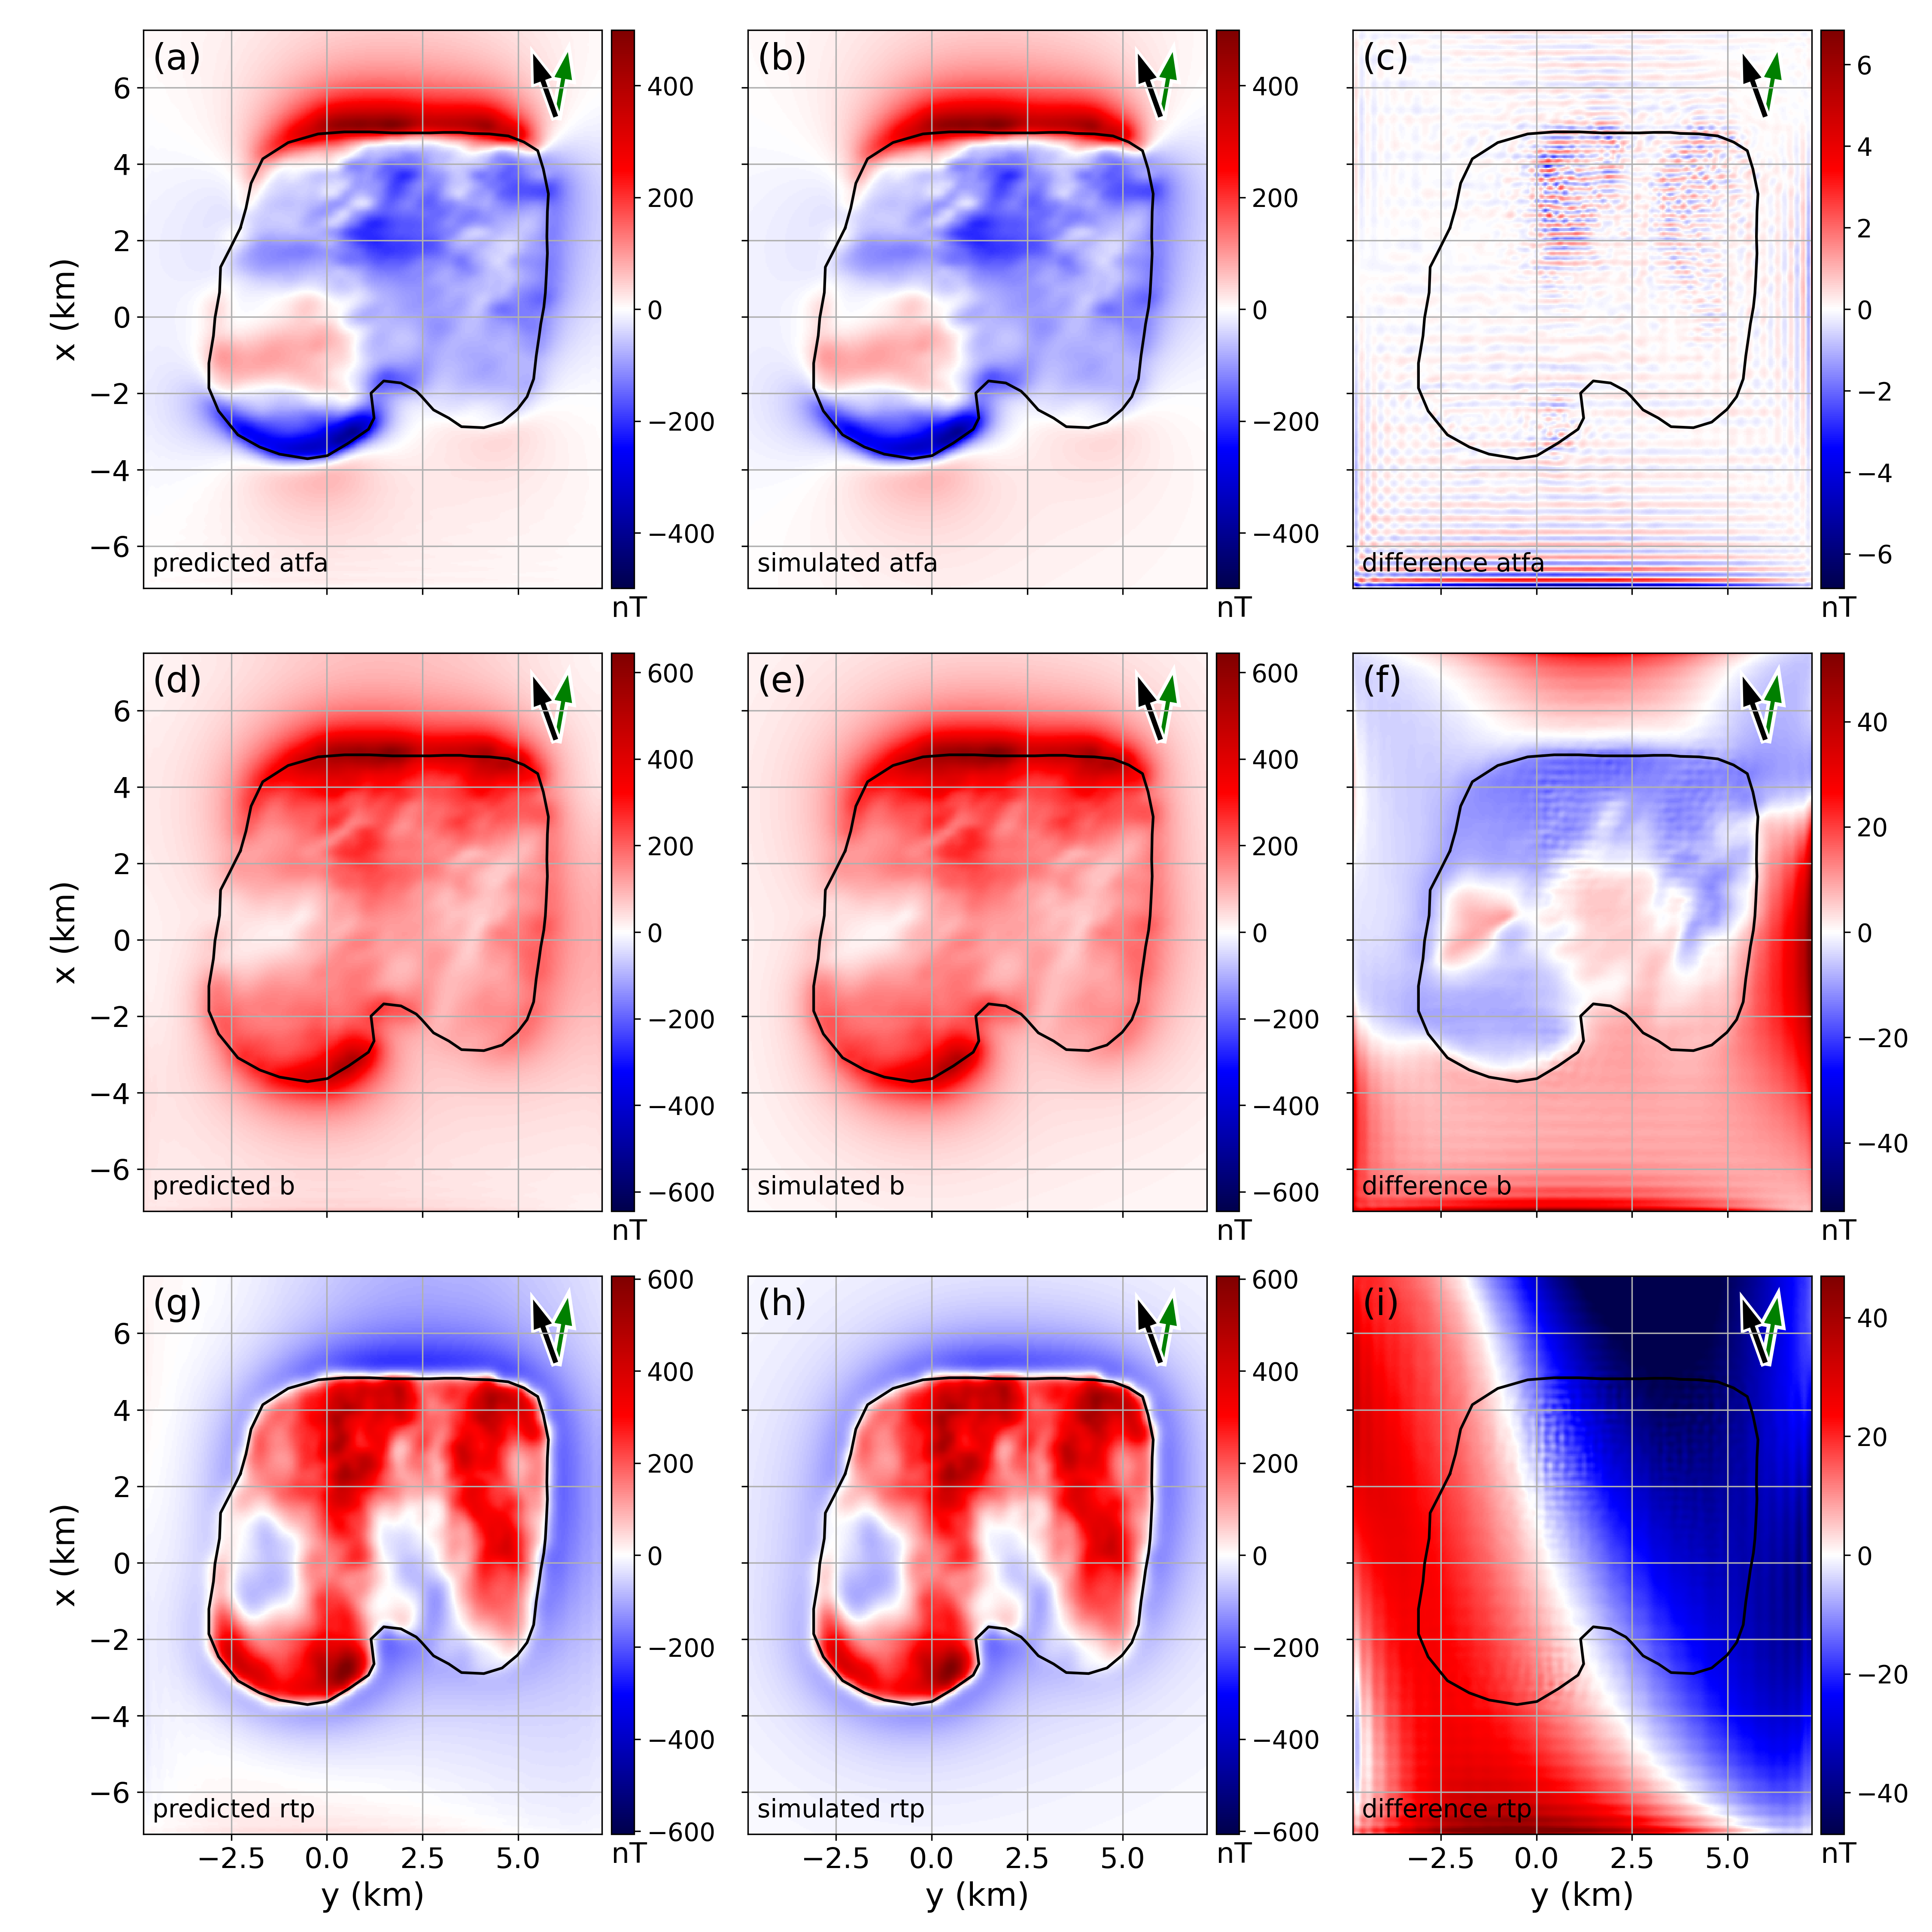
\includegraphics[width=0.8\textwidth]{Figure_S10.png}
	\caption{%
		Comparison between the simulated fields and those predicted by the estimated equivalent layer shown in Figure \mainref{fig:Figure4}b.
	}
	\label{S-fig:FigureS10}
\end{figure}

\begin{figure}[h]
	\centering
	\noindent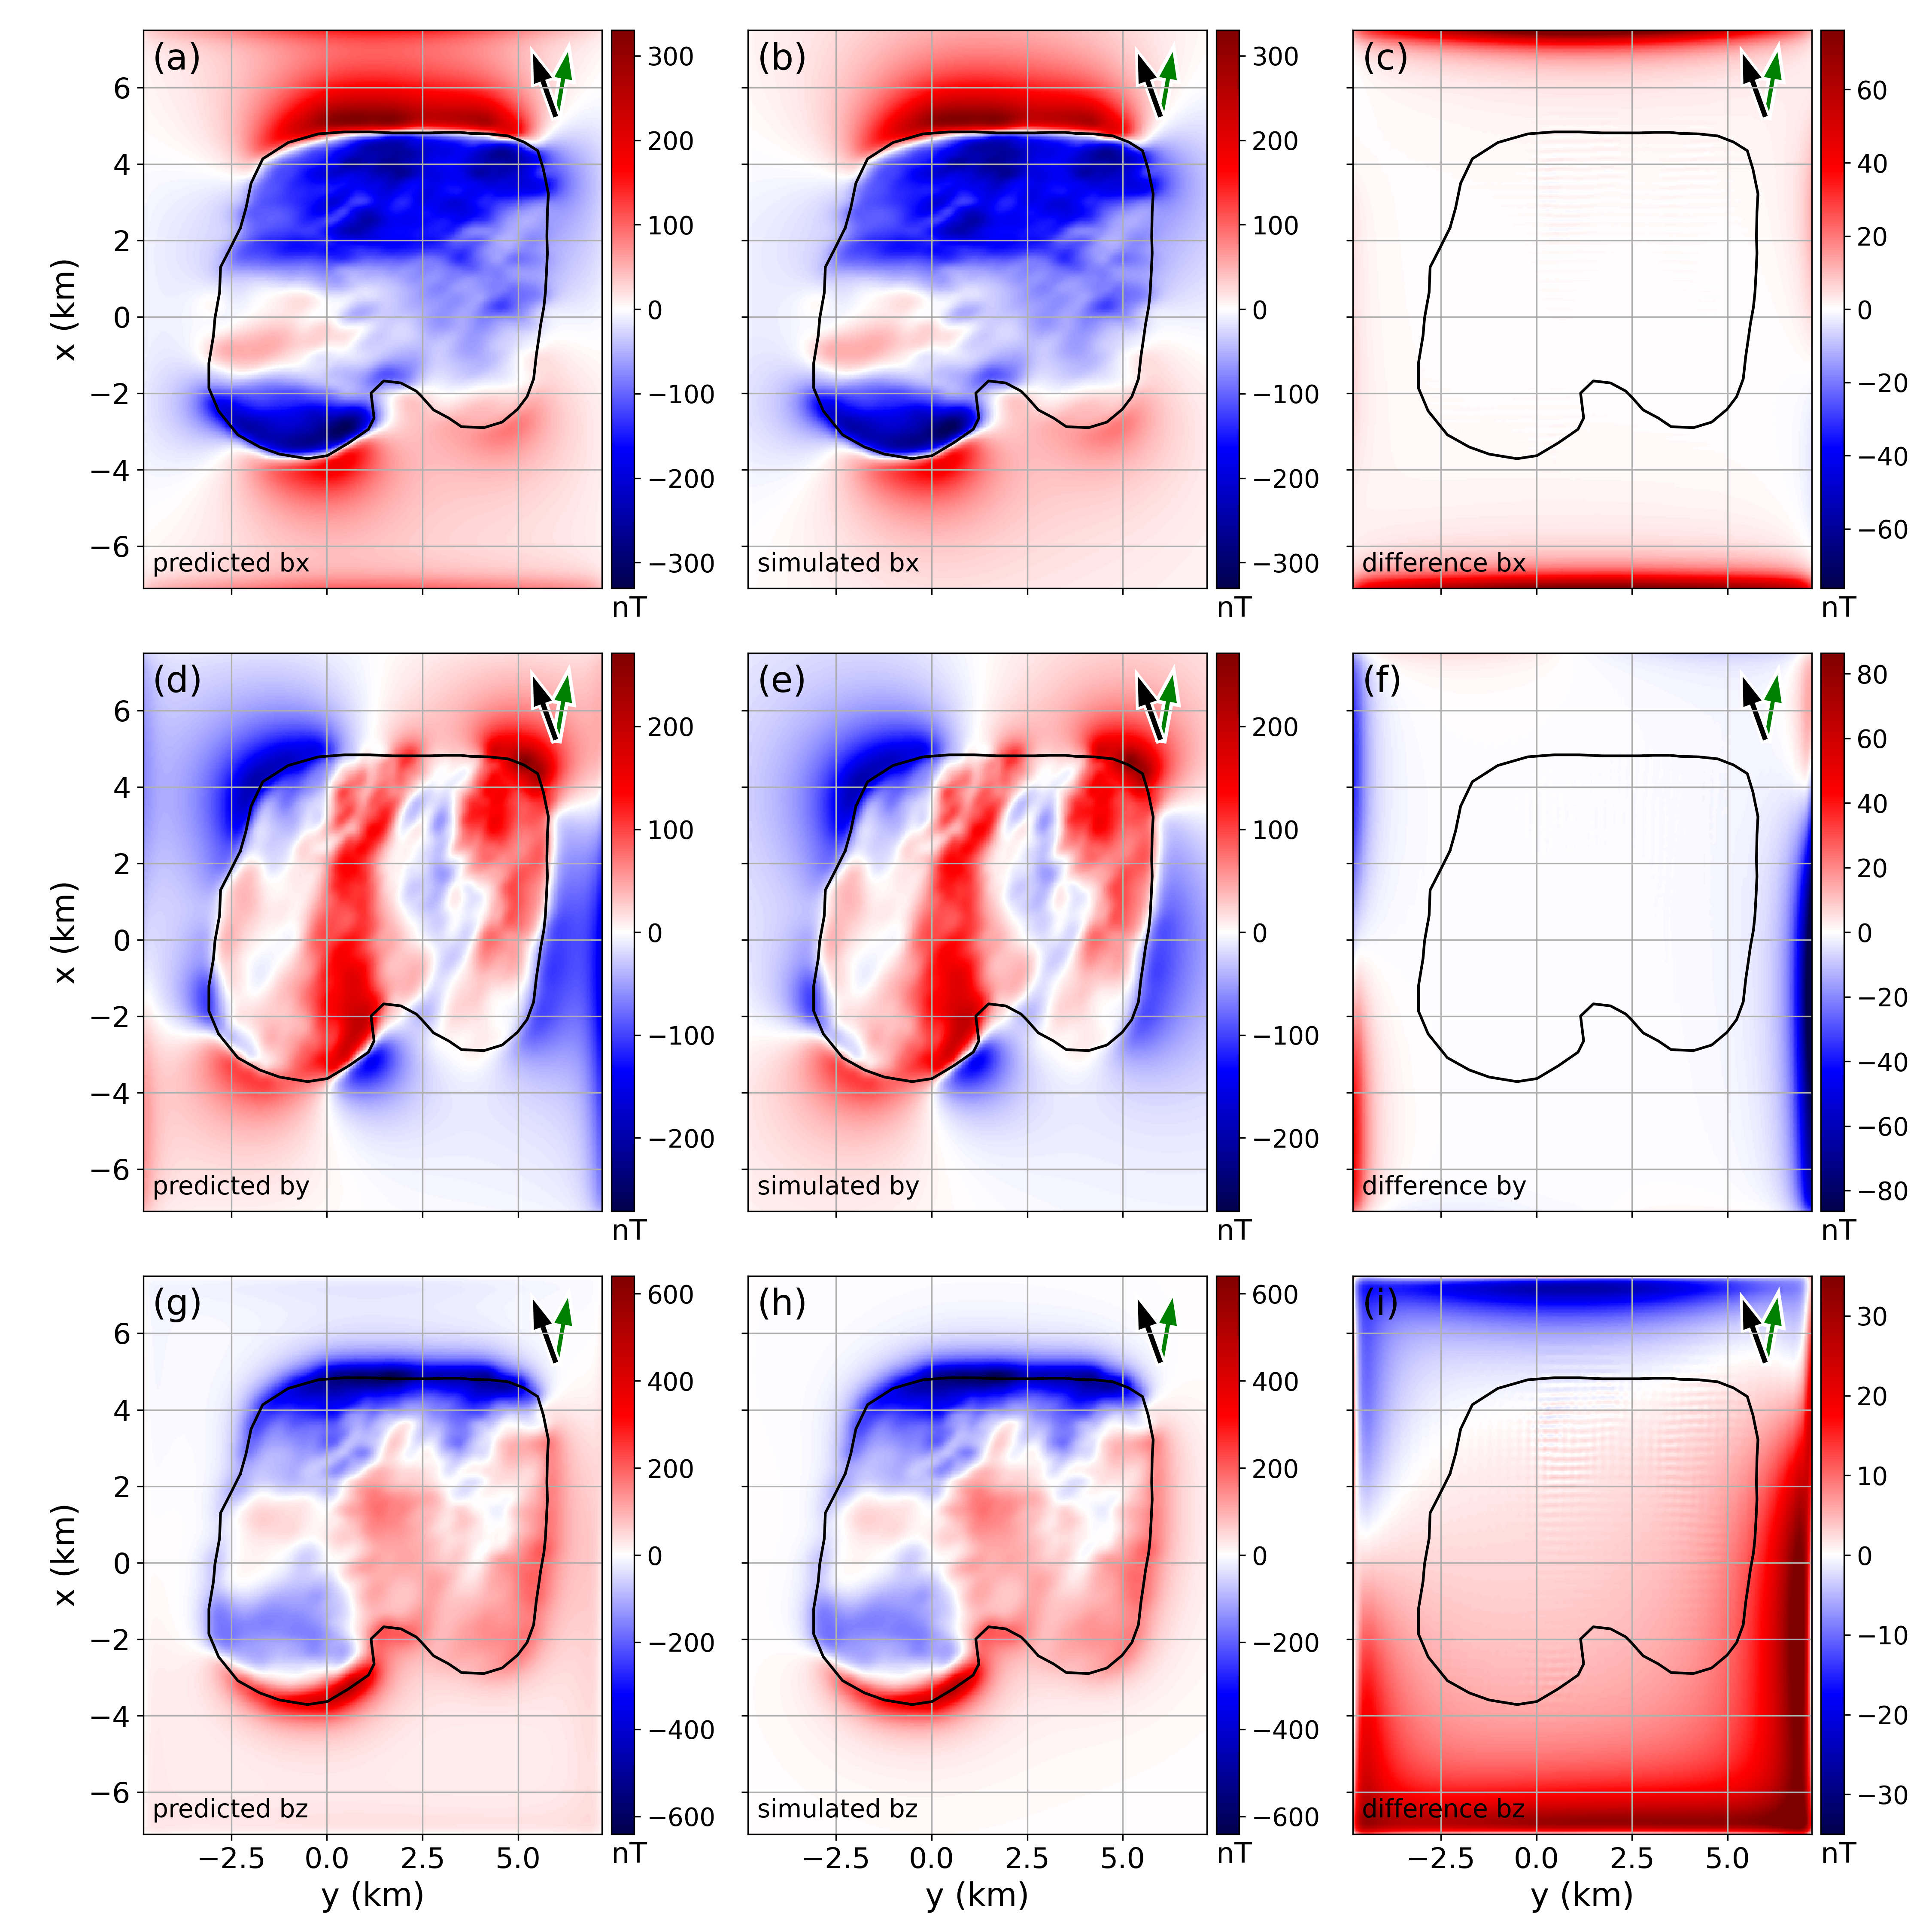
\includegraphics[width=0.8\textwidth]{Figure_S11.png}
	\caption{%
		Comparison between the simulated fields and those predicted by the estimated equivalent layer shown in Figure \mainref{fig:Figure4}e.
	}
	\label{S-fig:FigureS11}
\end{figure}

\begin{figure}[h]
	\centering
	\noindent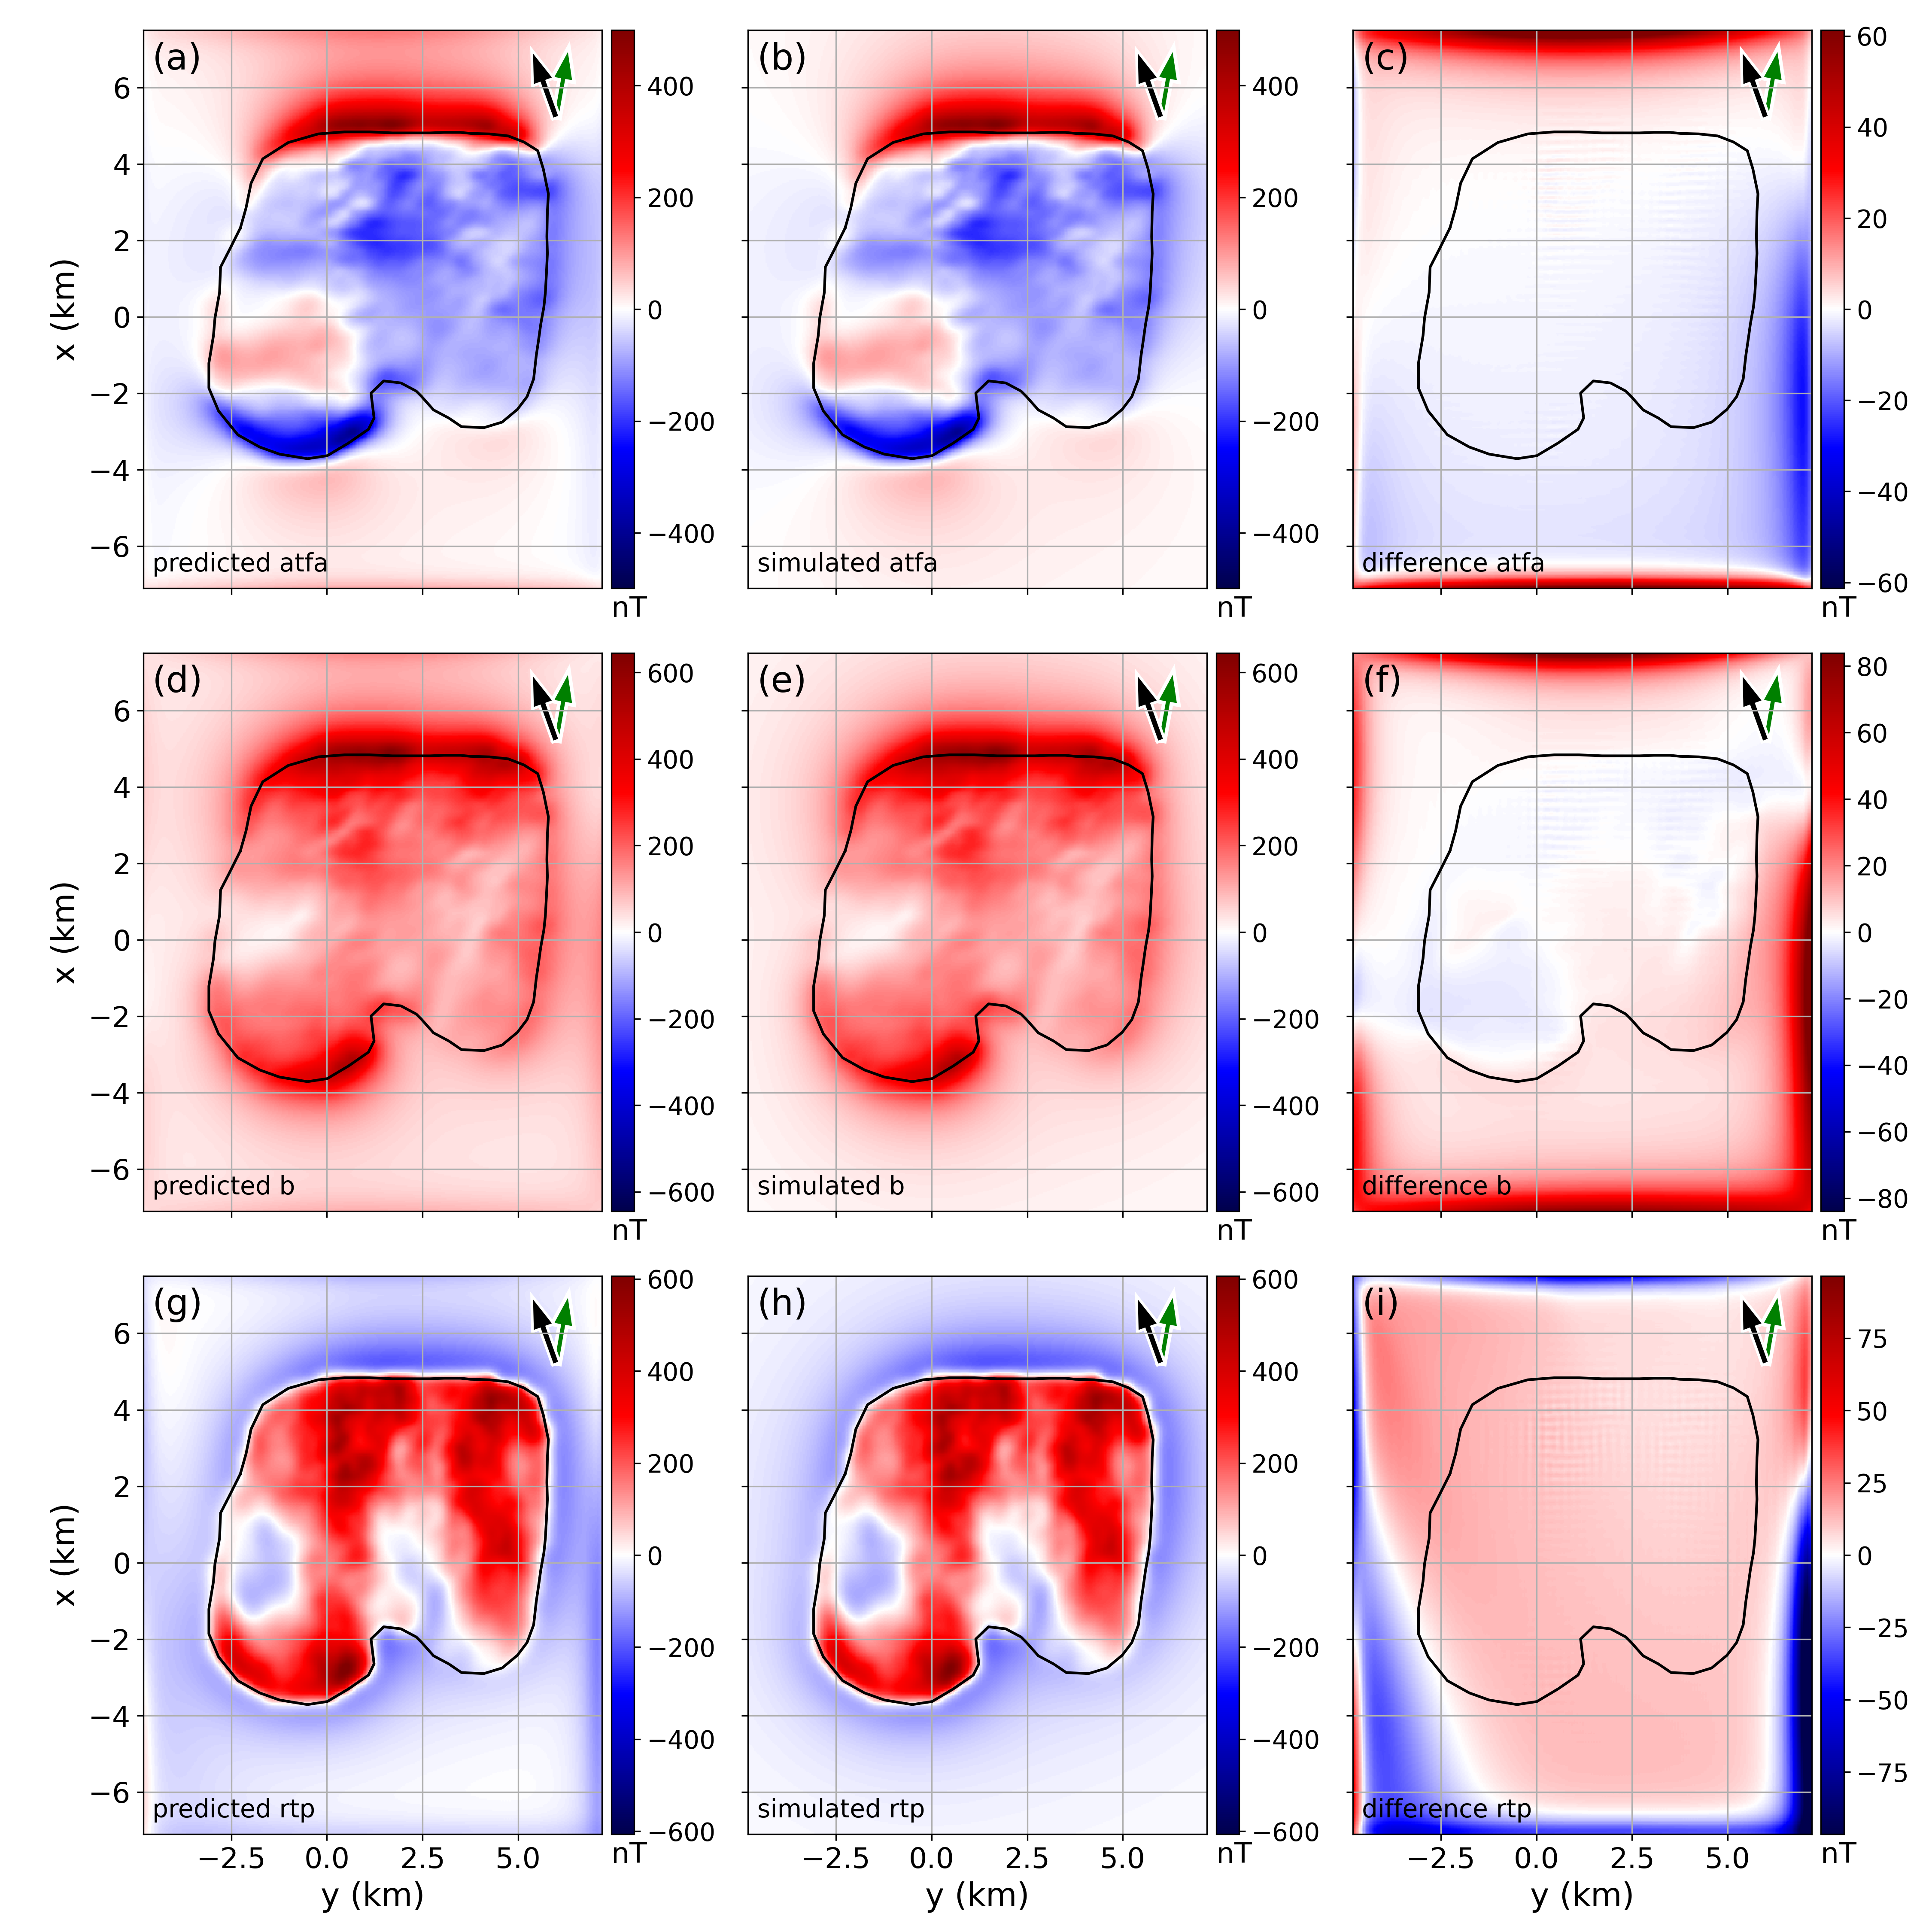
\includegraphics[width=0.8\textwidth]{Figure_S12.png}
	\caption{%
		Comparison between the simulated fields and those predicted by the estimated equivalent layer shown in Figure \mainref{fig:Figure4}e.
	}
	\label{S-fig:FigureS12}
\end{figure}

\begin{figure}[h]
	\centering
	\noindent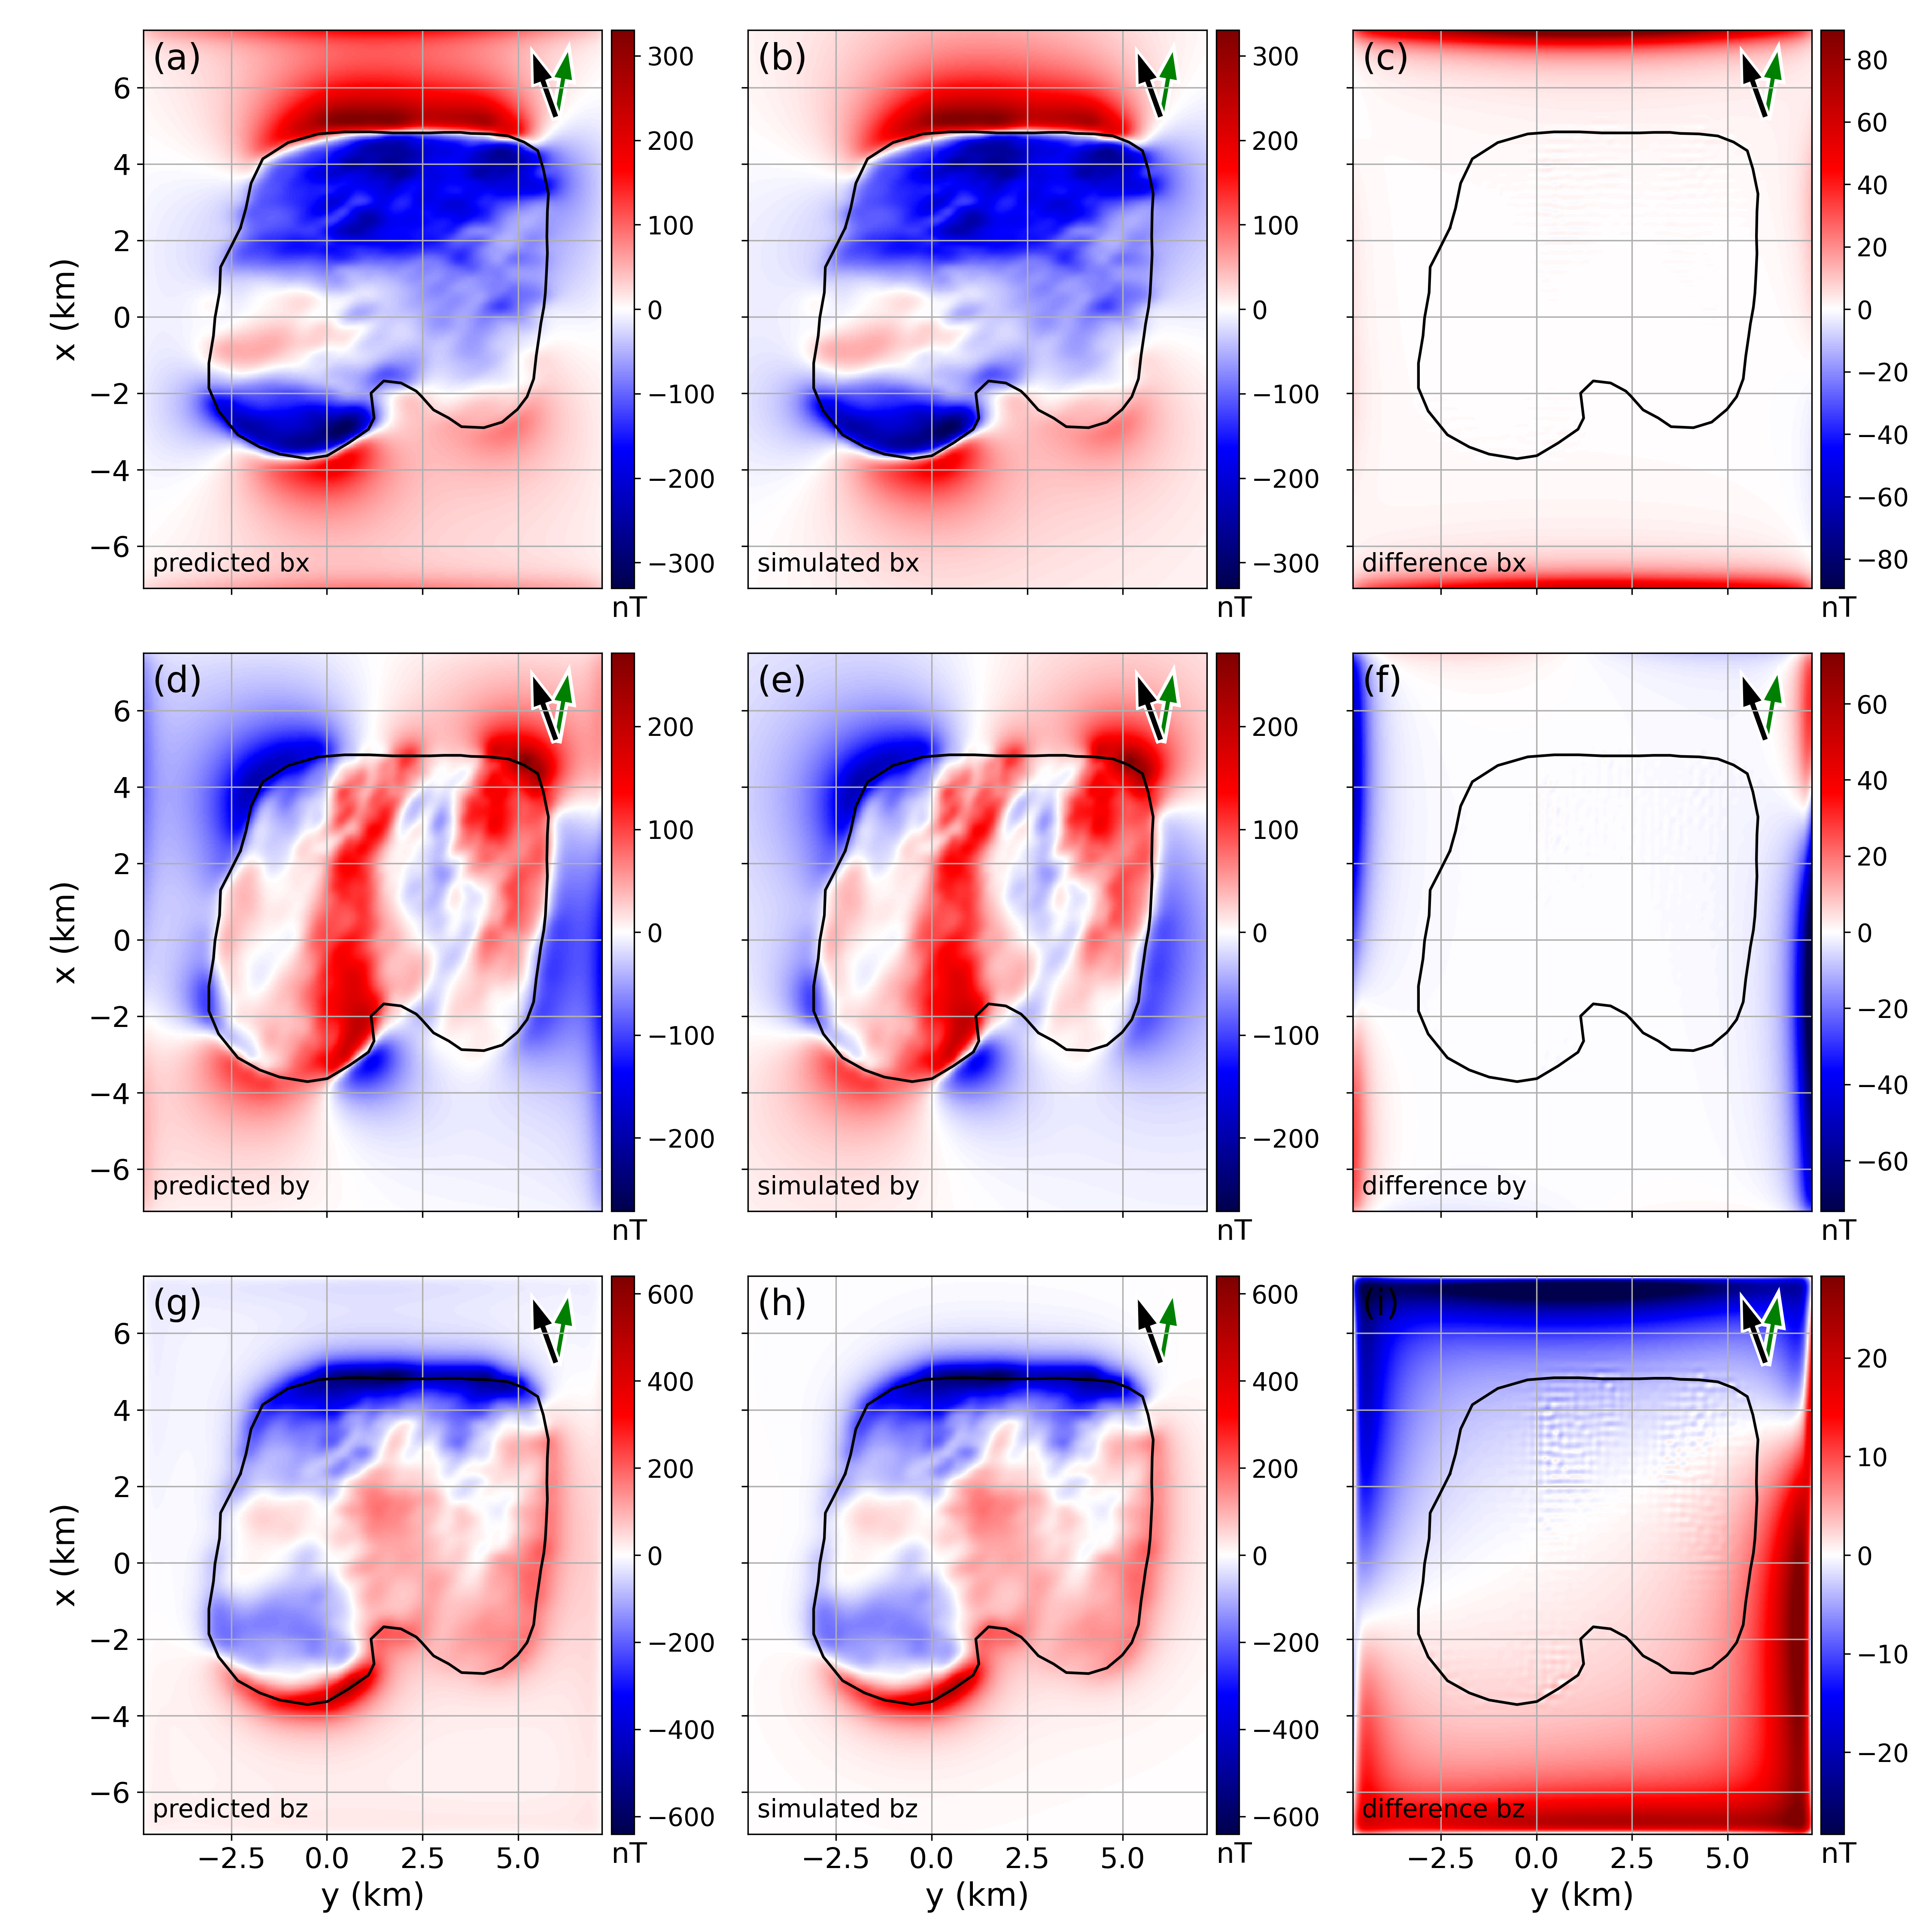
\includegraphics[width=0.8\textwidth]{Figure_S13.png}
	\caption{%
		Comparison between the simulated fields and those predicted by the estimated equivalent layer shown in Figure \mainref{fig:Figure4}h.
	}
	\label{S-fig:FigureS13}
\end{figure}

\begin{figure}[h]
	\centering
	\noindent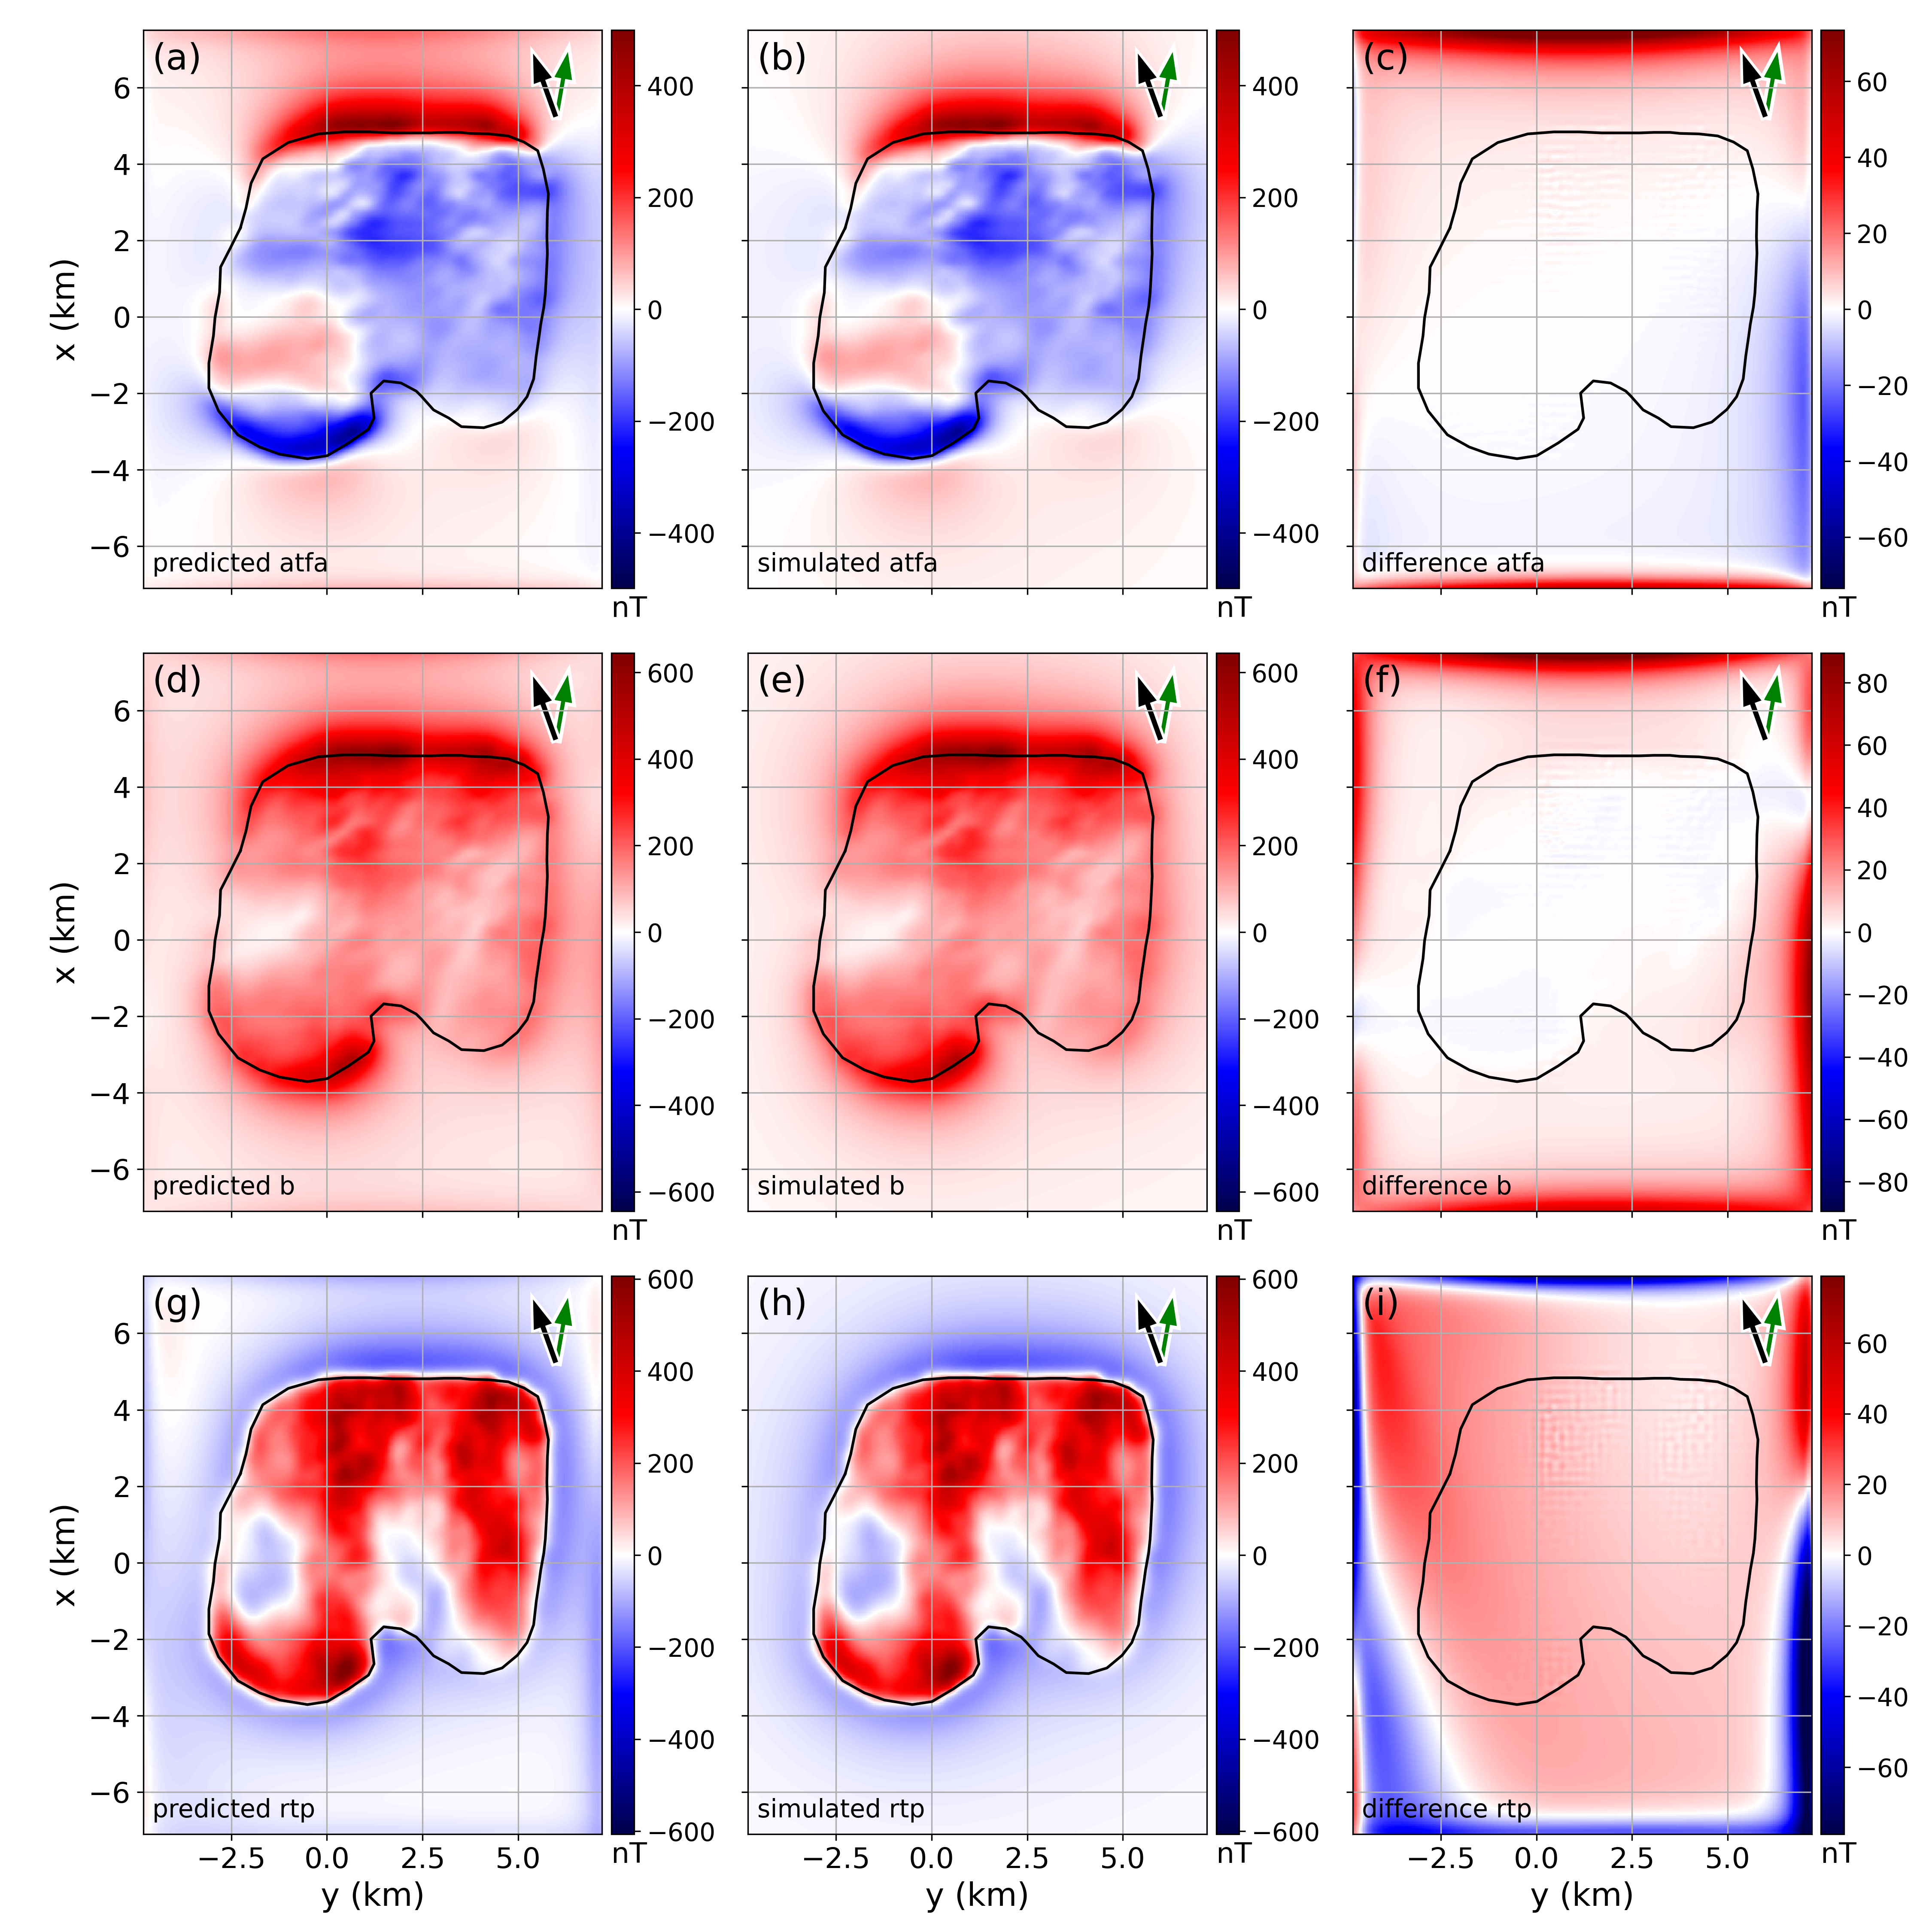
\includegraphics[width=0.8\textwidth]{Figure_S14.png}
	\caption{%
		Comparison between the simulated fields and those predicted by the estimated equivalent layer shown in Figure \mainref{fig:Figure4}h.
	}
	\label{S-fig:FigureS14}
\end{figure}

\begin{figure}[h]
	\centering
	\noindent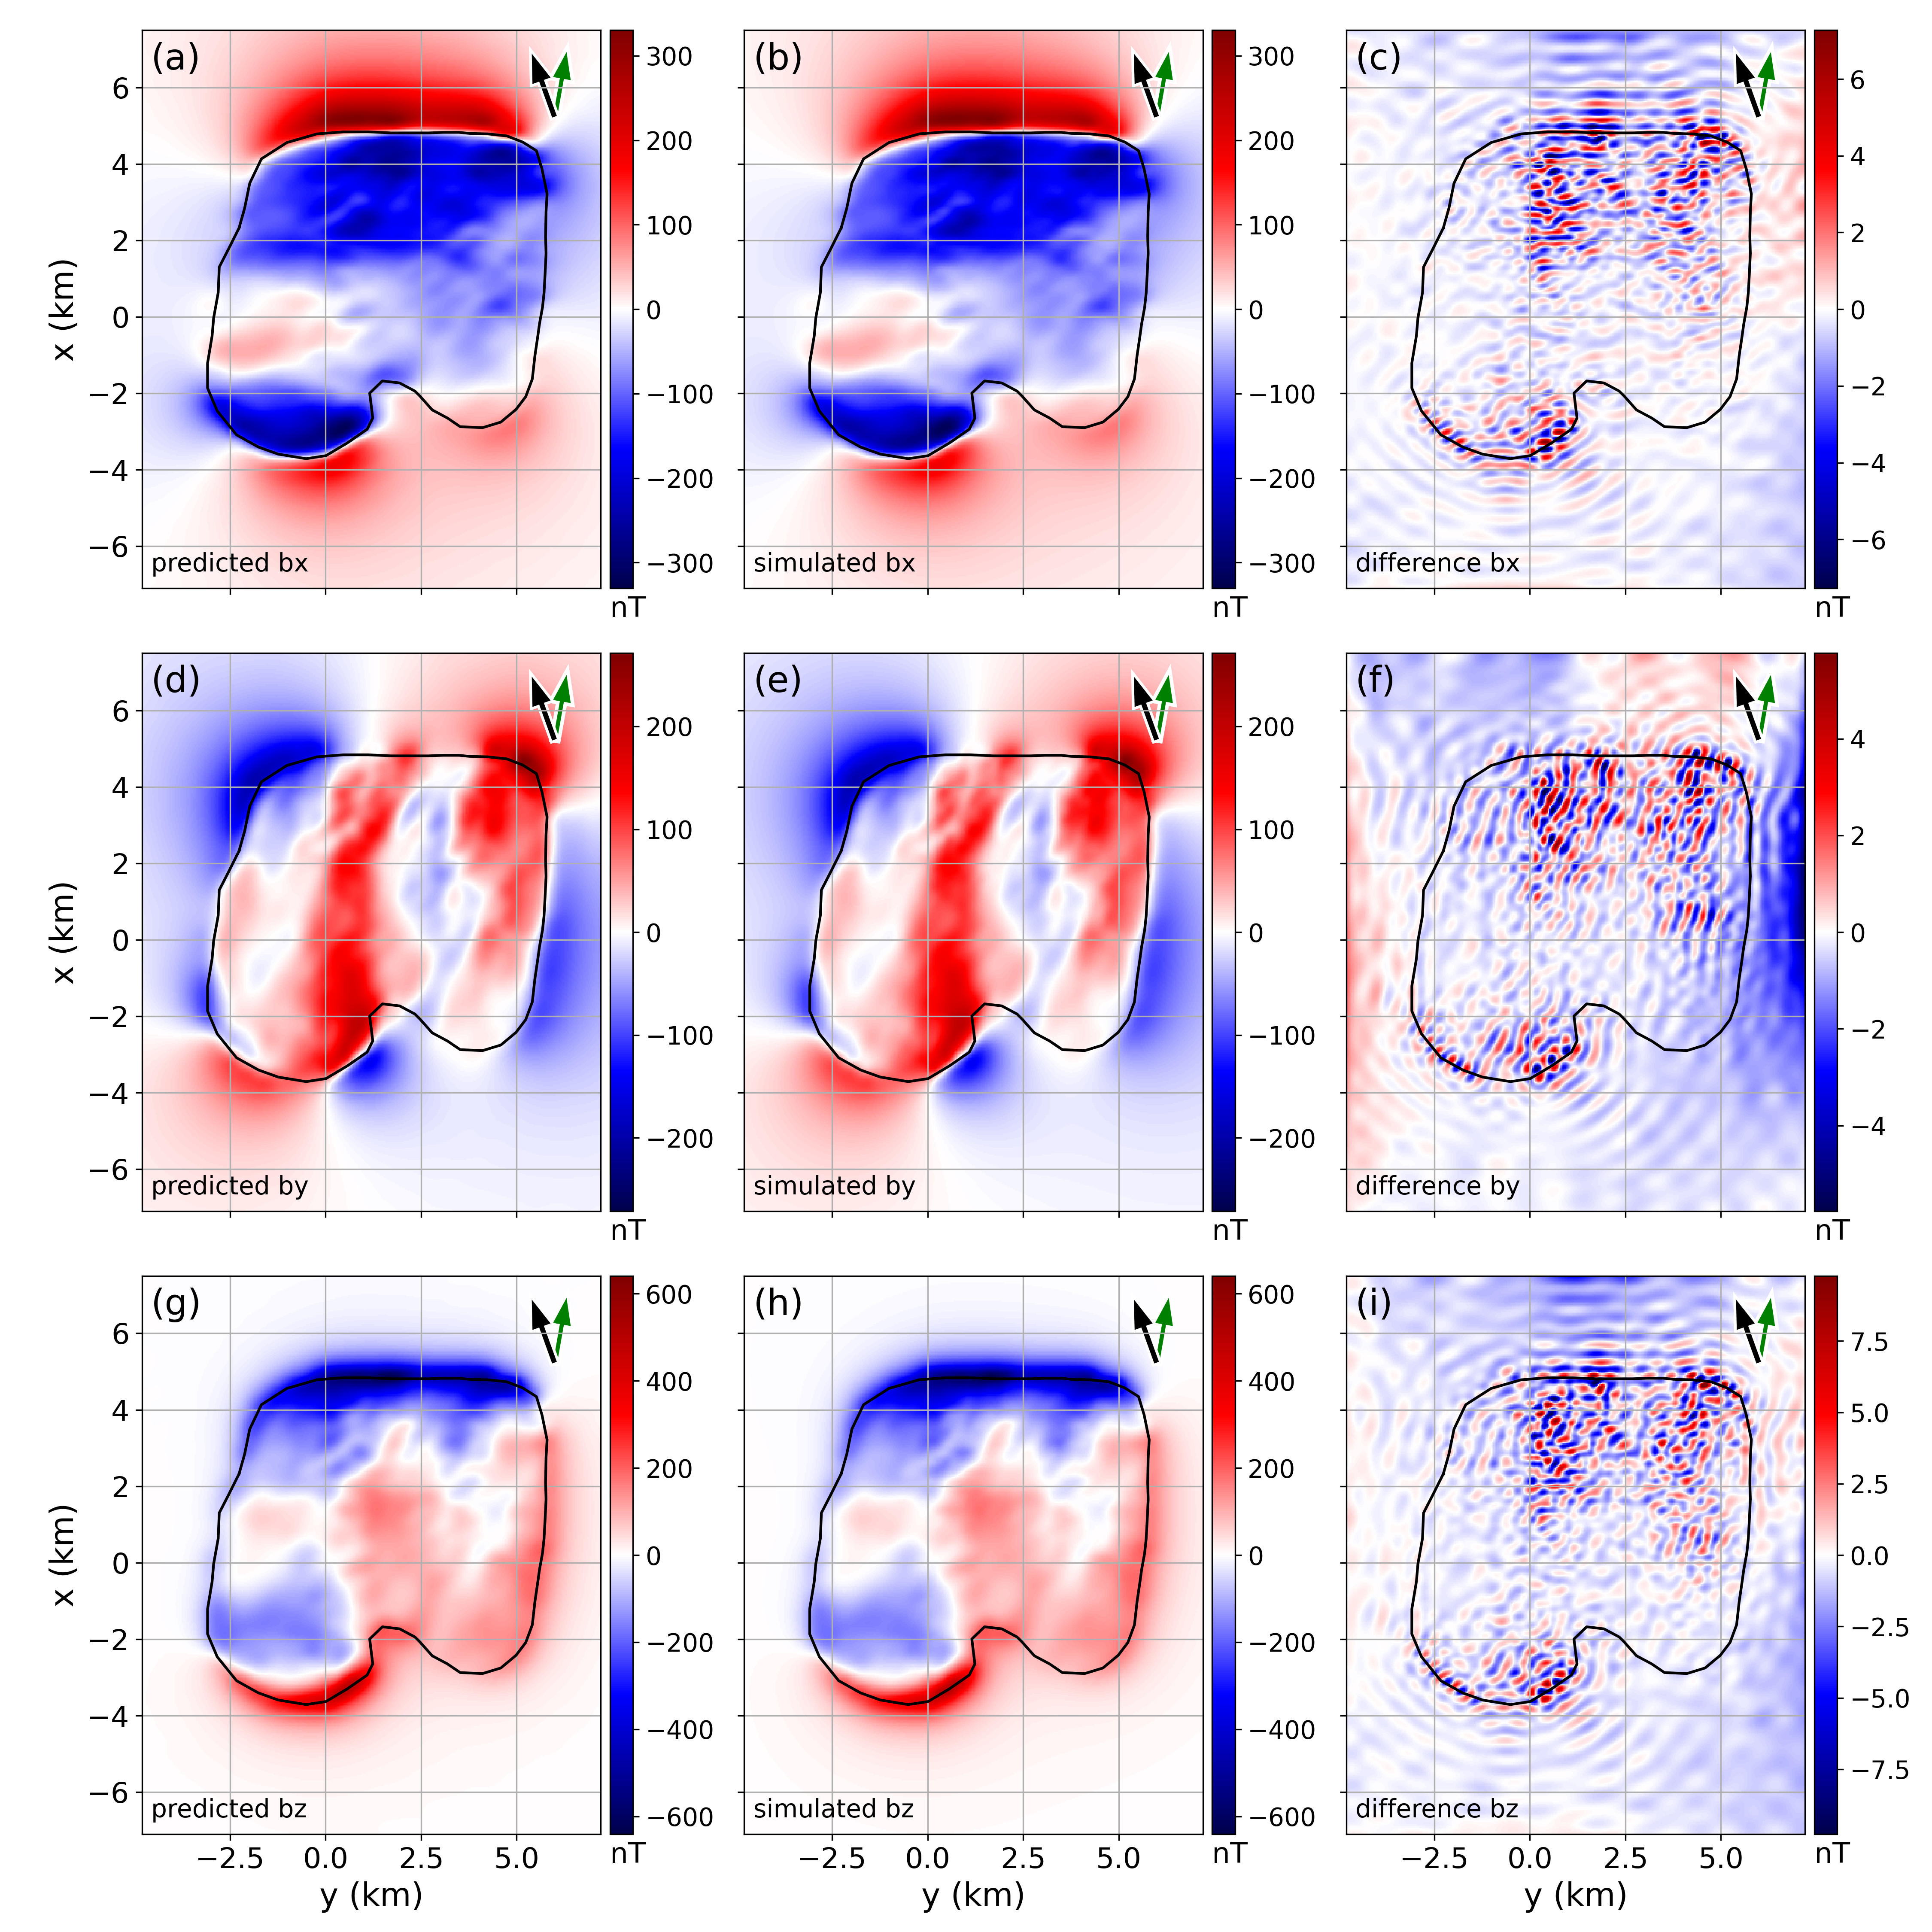
\includegraphics[width=0.8\textwidth]{Figure_S15.png}
	\caption{%
		Comparison between the simulated fields and those predicted by the estimated equivalent layer shown in Figure \mainref{fig:Figure4}c.
	}
	\label{S-fig:FigureS15}
\end{figure}

\begin{figure}[h]
	\centering
	\noindent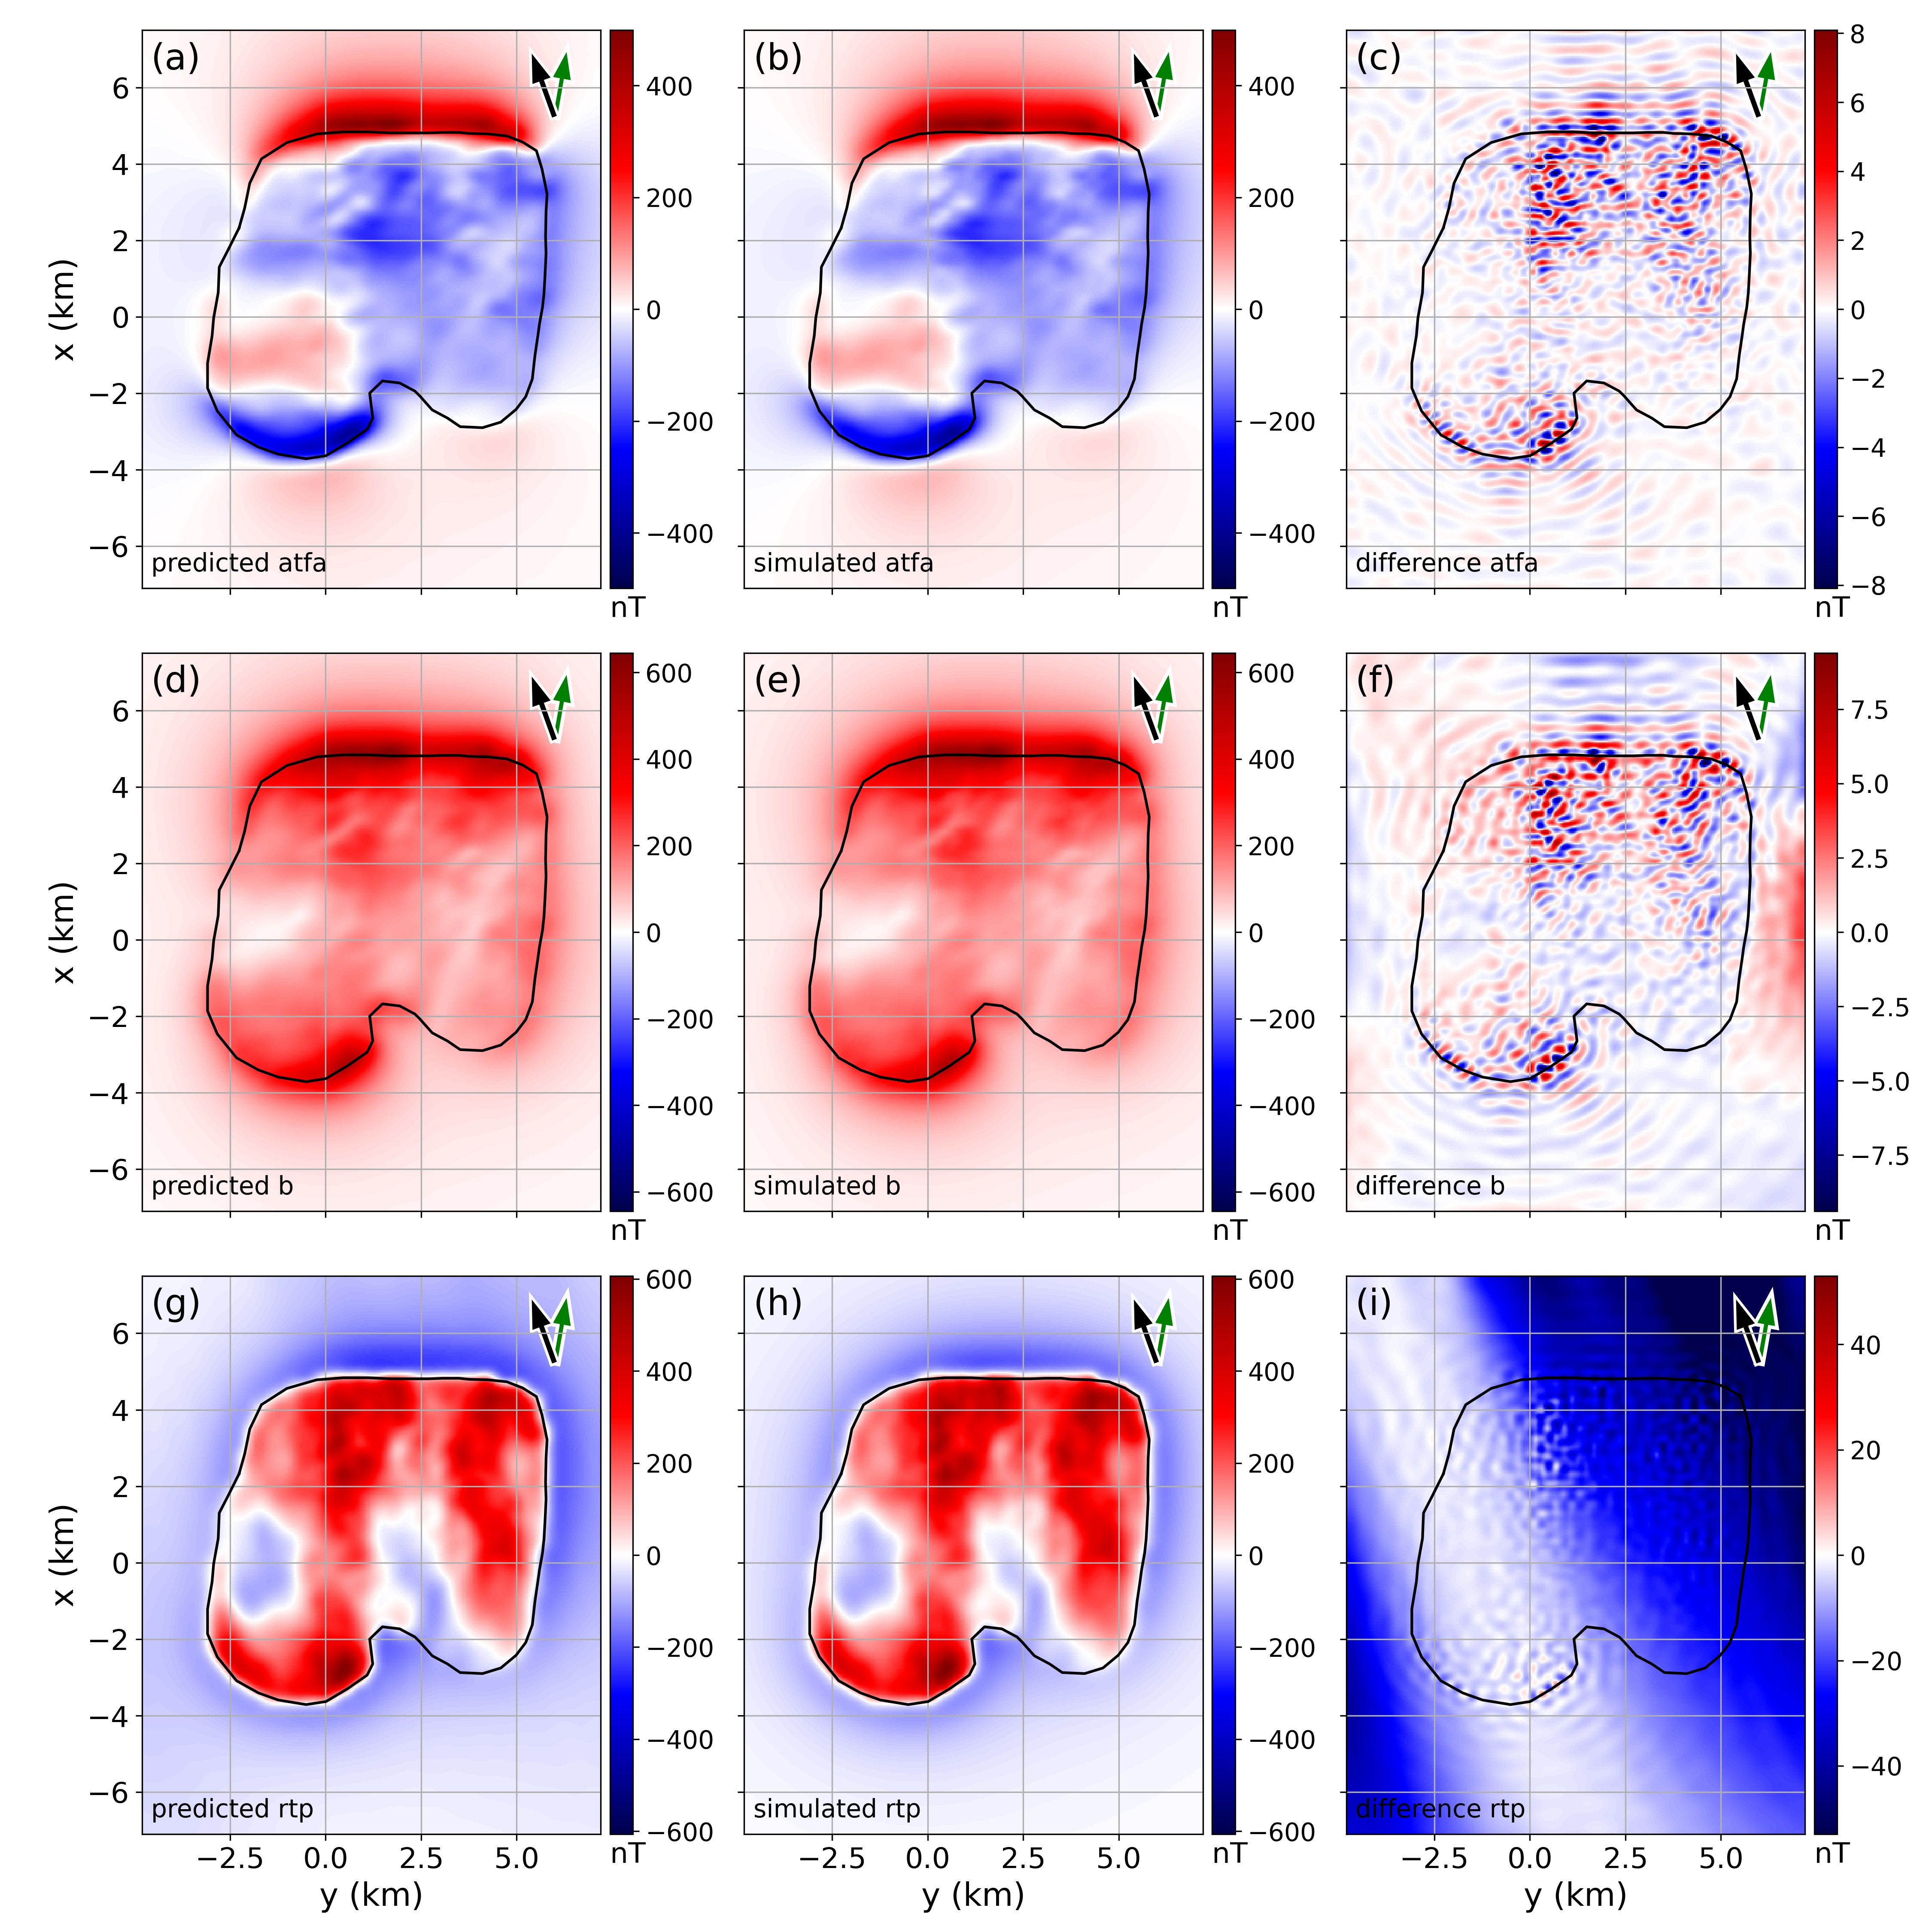
\includegraphics[width=0.8\textwidth]{Figure_S16.png}
	\caption{%
		Comparison between the simulated fields and those predicted by the estimated equivalent layer shown in Figure \mainref{fig:Figure4}c.
	}
	\label{S-fig:FigureS16}
\end{figure}

\begin{figure}[h]
	\centering
	\noindent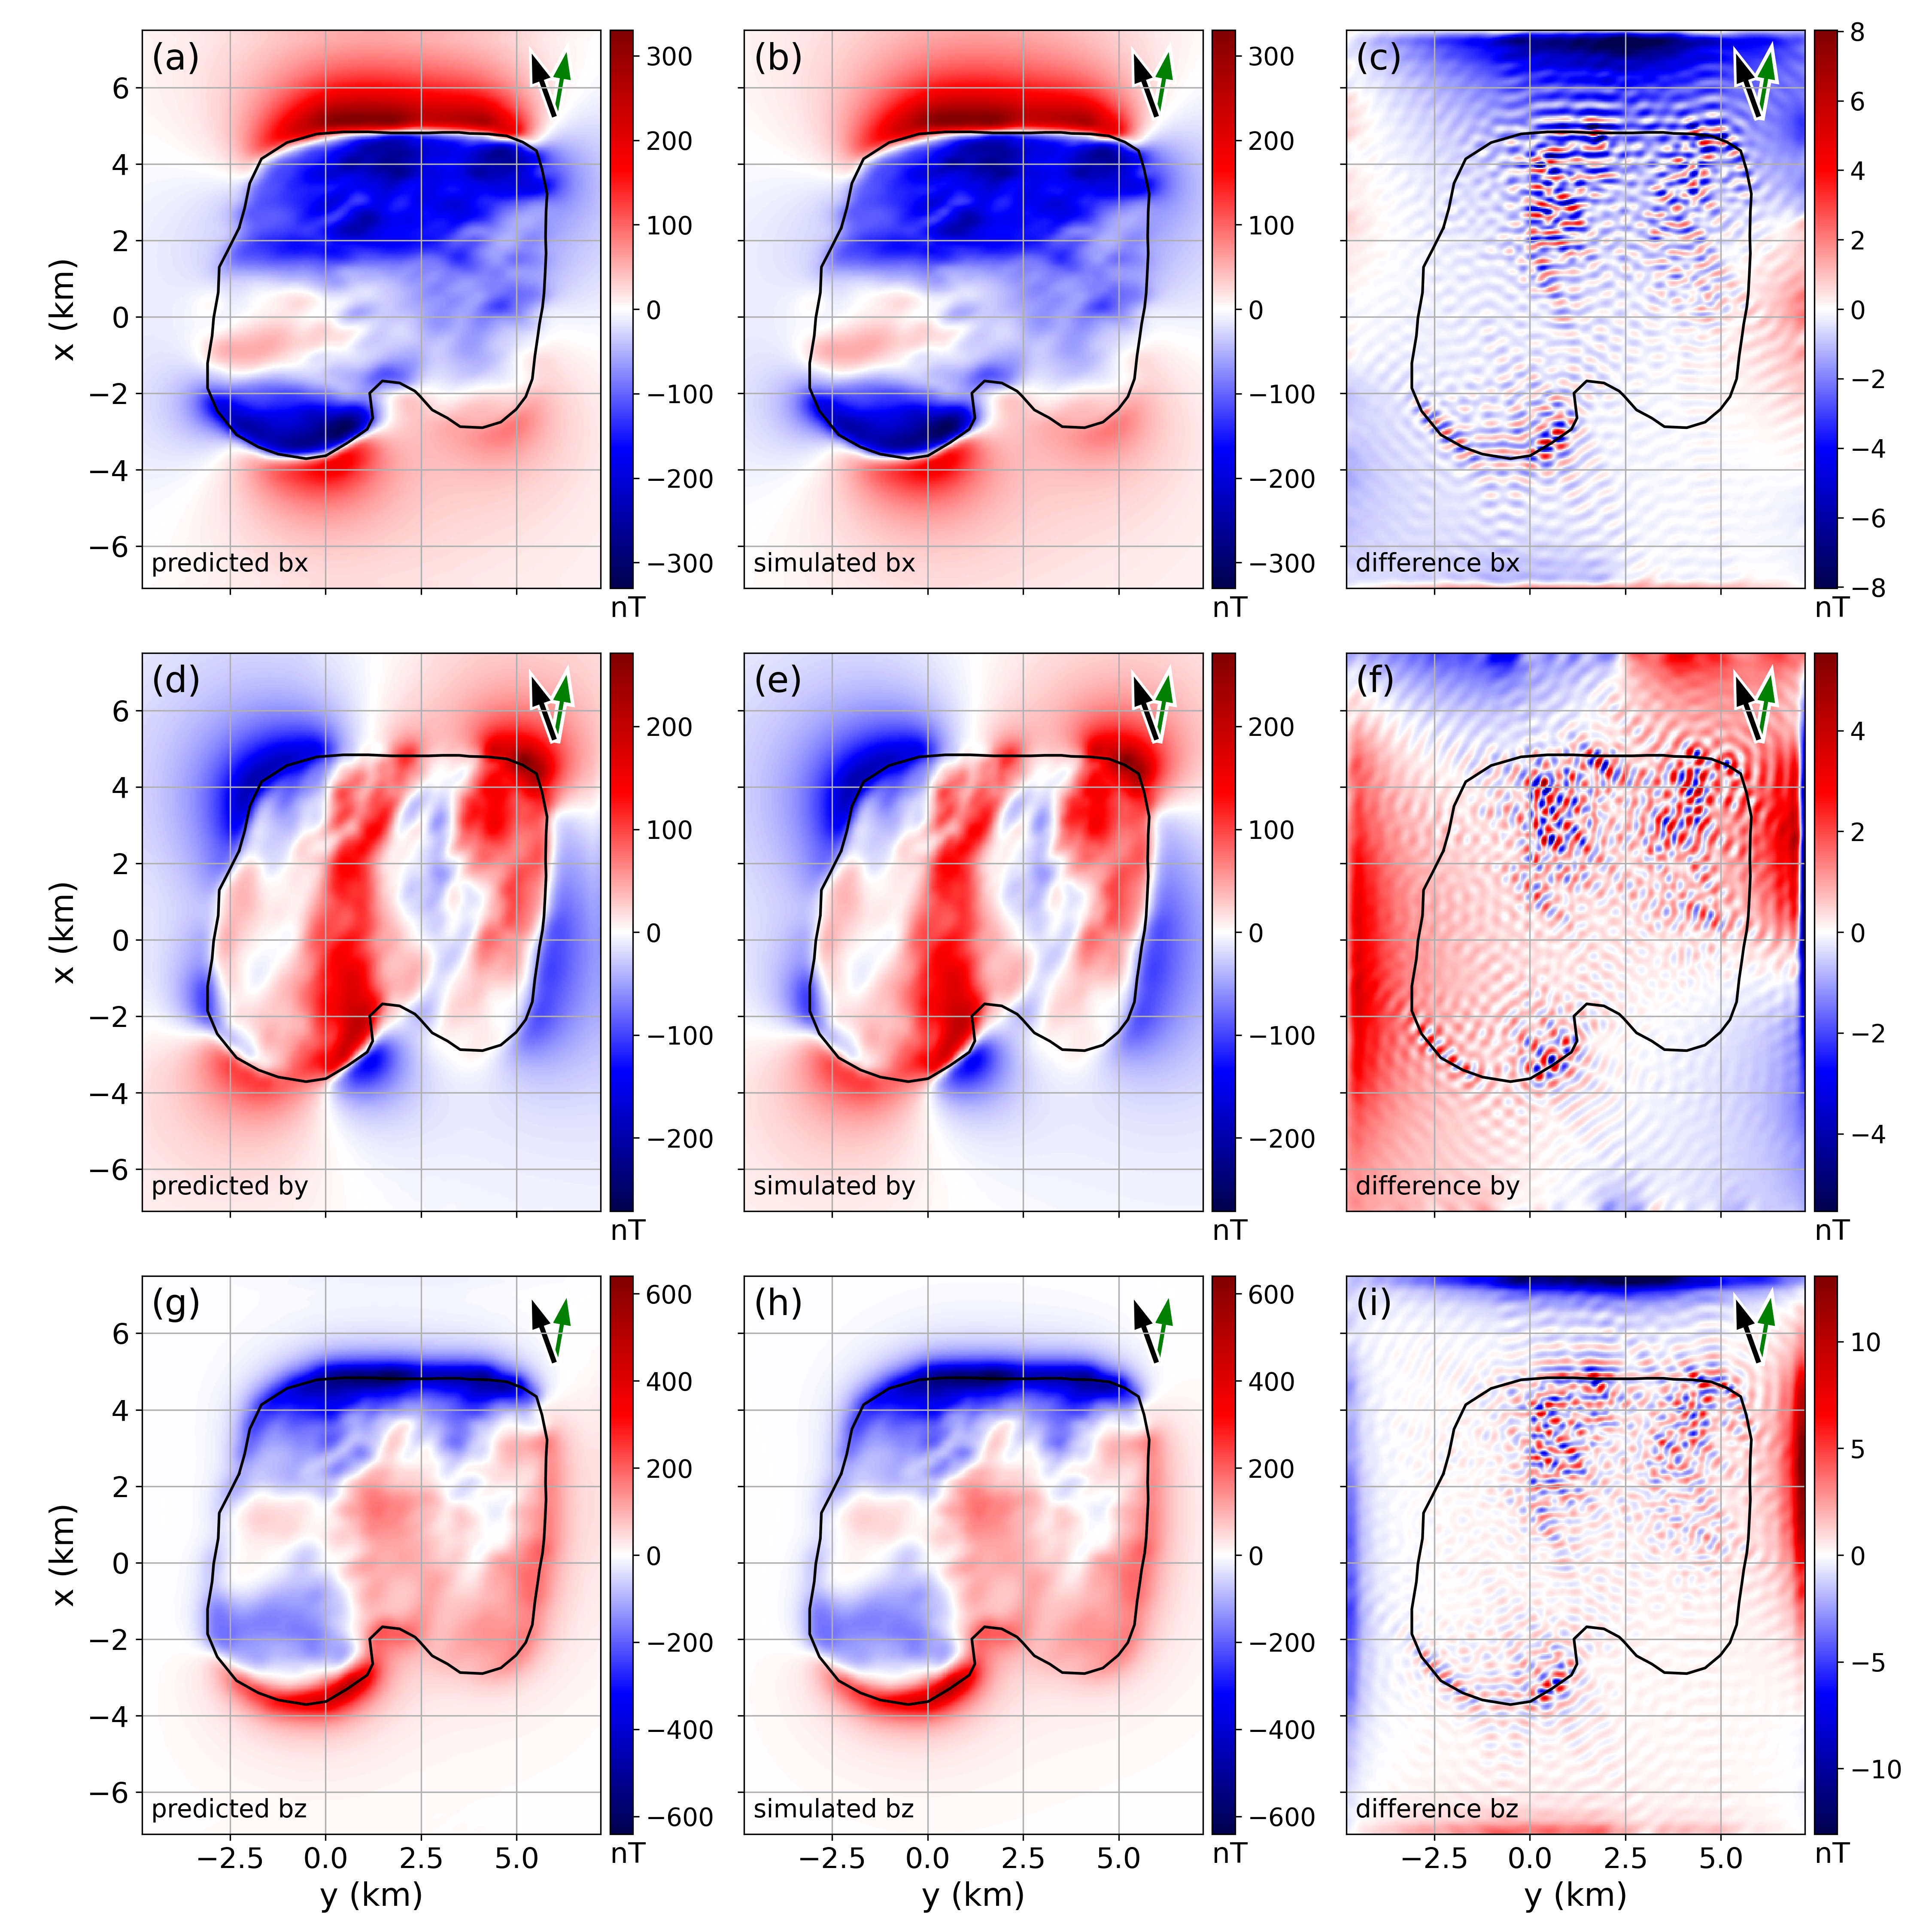
\includegraphics[width=0.8\textwidth]{Figure_S17.png}
	\caption{%
		Comparison between the simulated fields and those predicted by the estimated equivalent layer shown in Figure \mainref{fig:Figure4}f.
	}
	\label{S-fig:FigureS17}
\end{figure}

\begin{figure}[h]
	\centering
	\noindent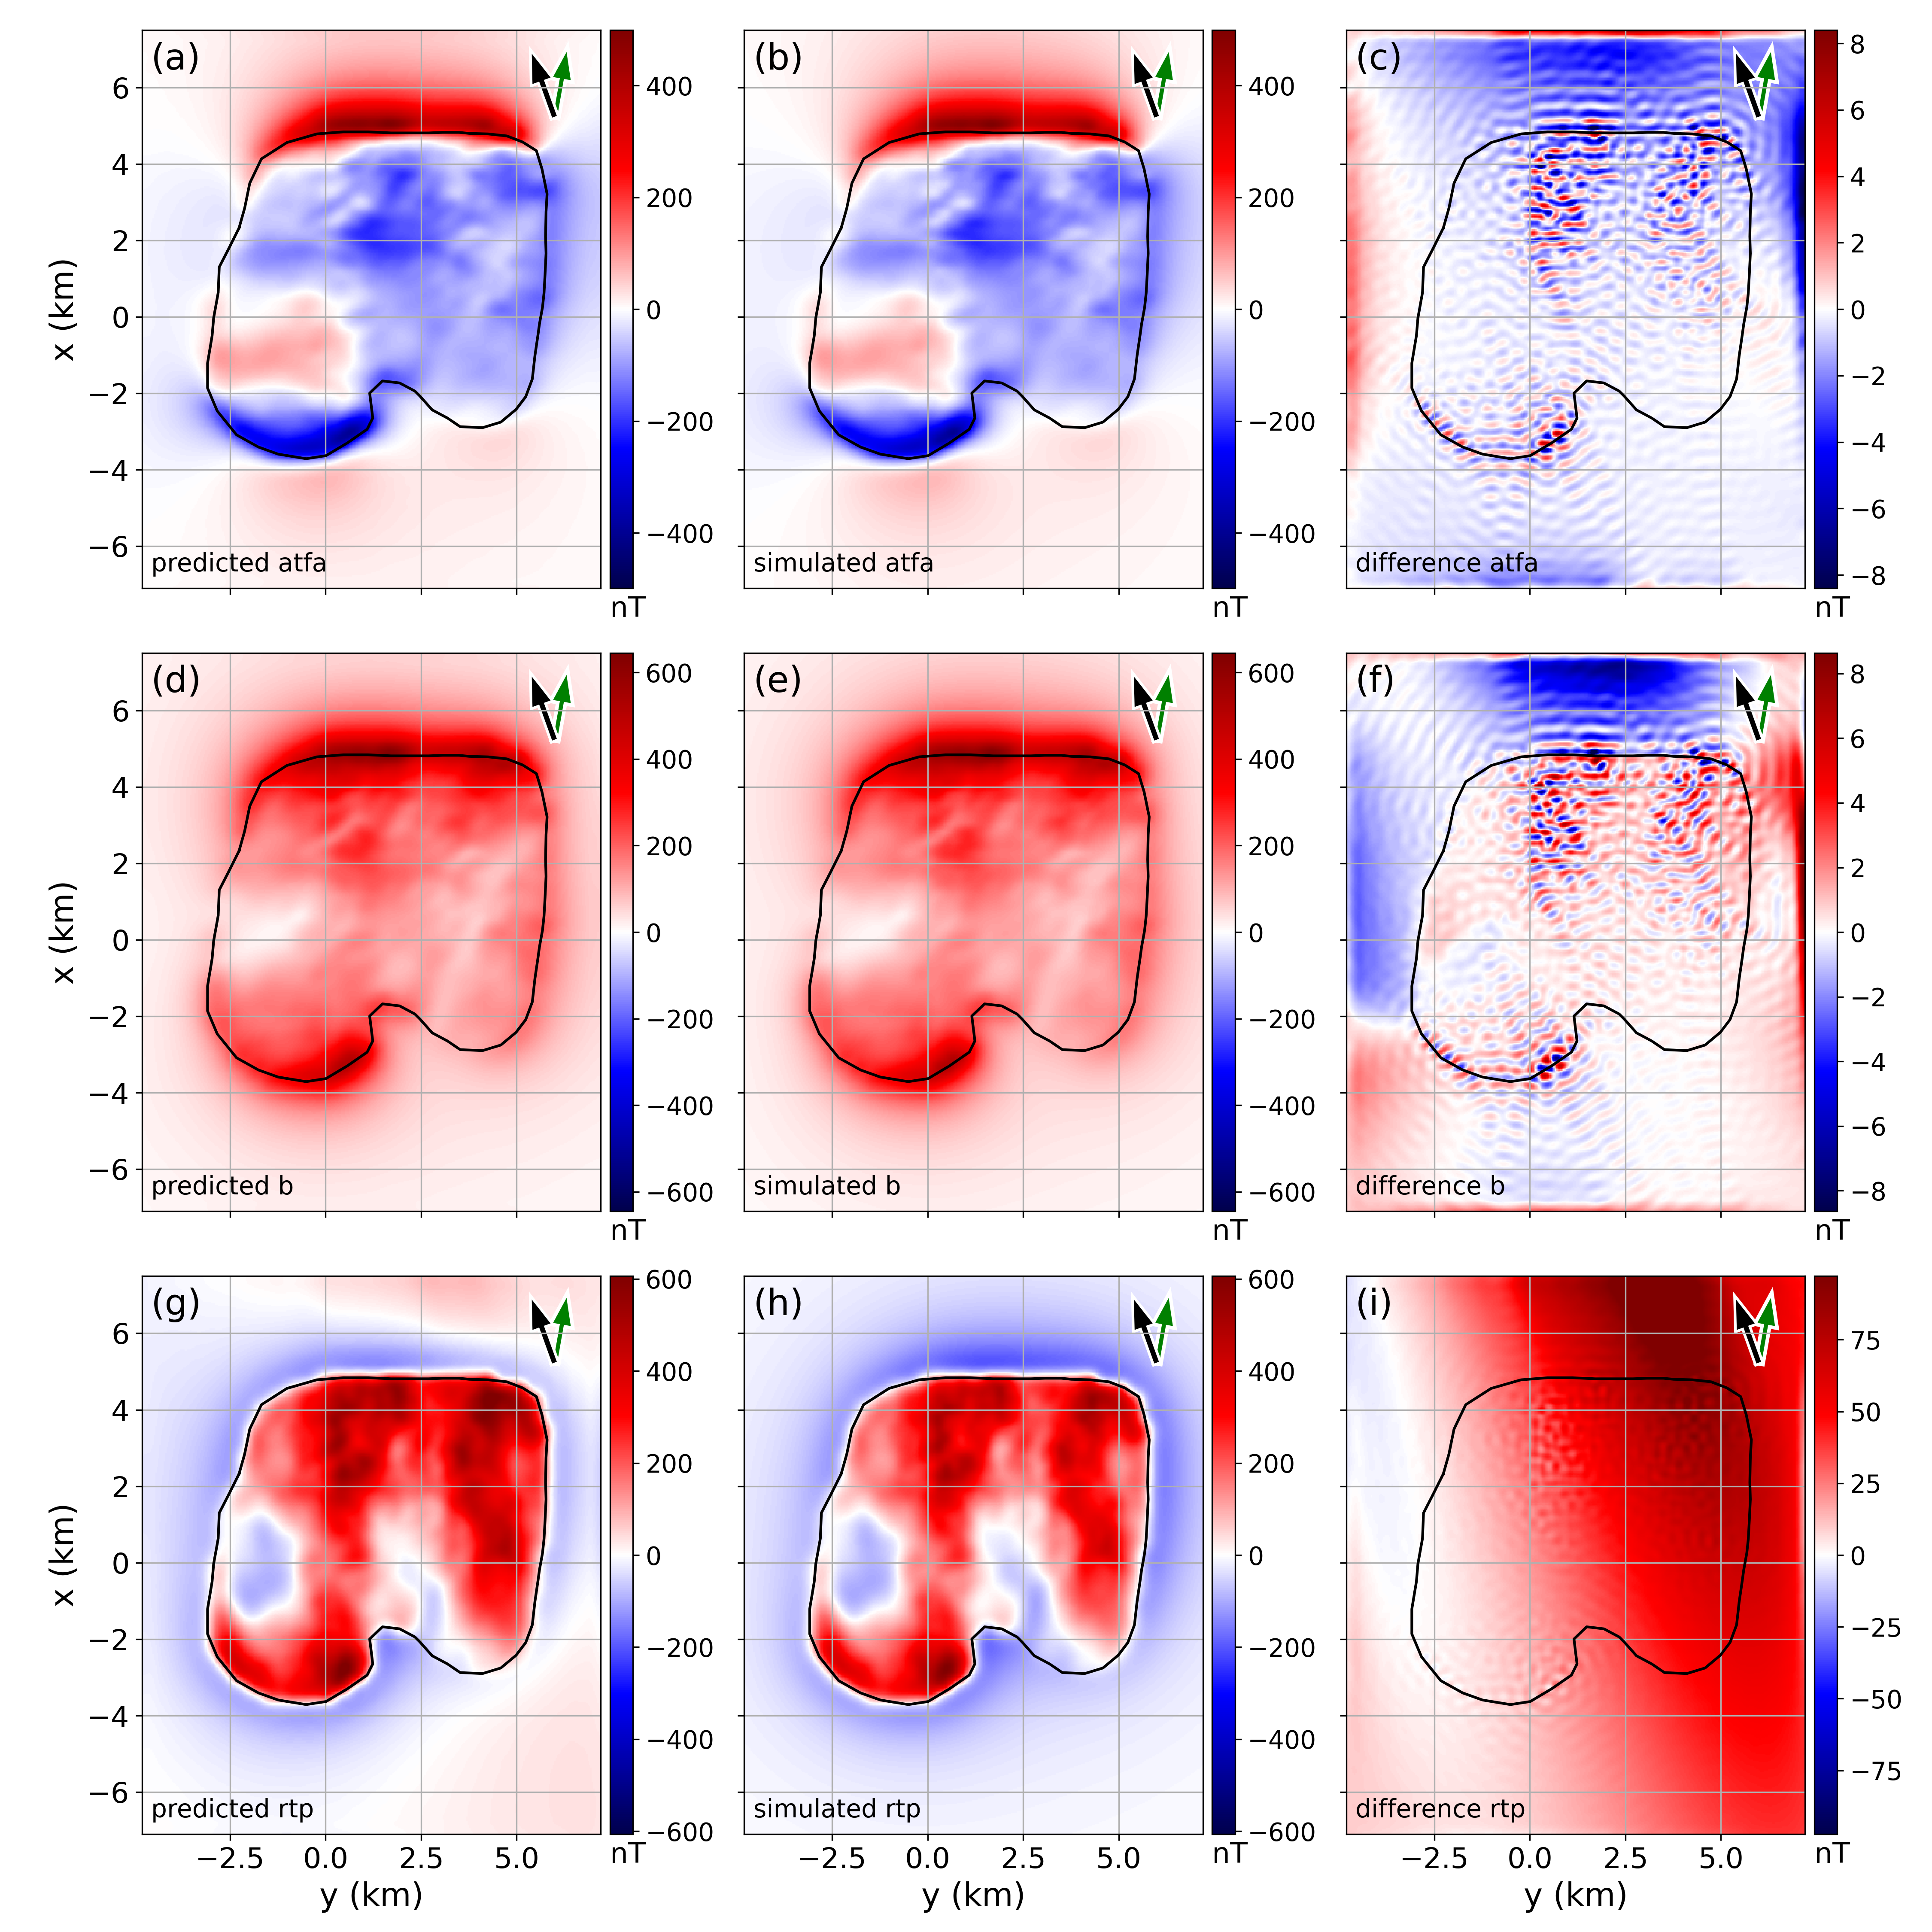
\includegraphics[width=0.8\textwidth]{Figure_S18.png}
	\caption{%
		Comparison between the simulated fields and those predicted by the estimated equivalent layer shown in Figure \mainref{fig:Figure4}f.
	}
	\label{S-fig:FigureS18}
\end{figure}

\begin{figure}[h]
	\centering
	\noindent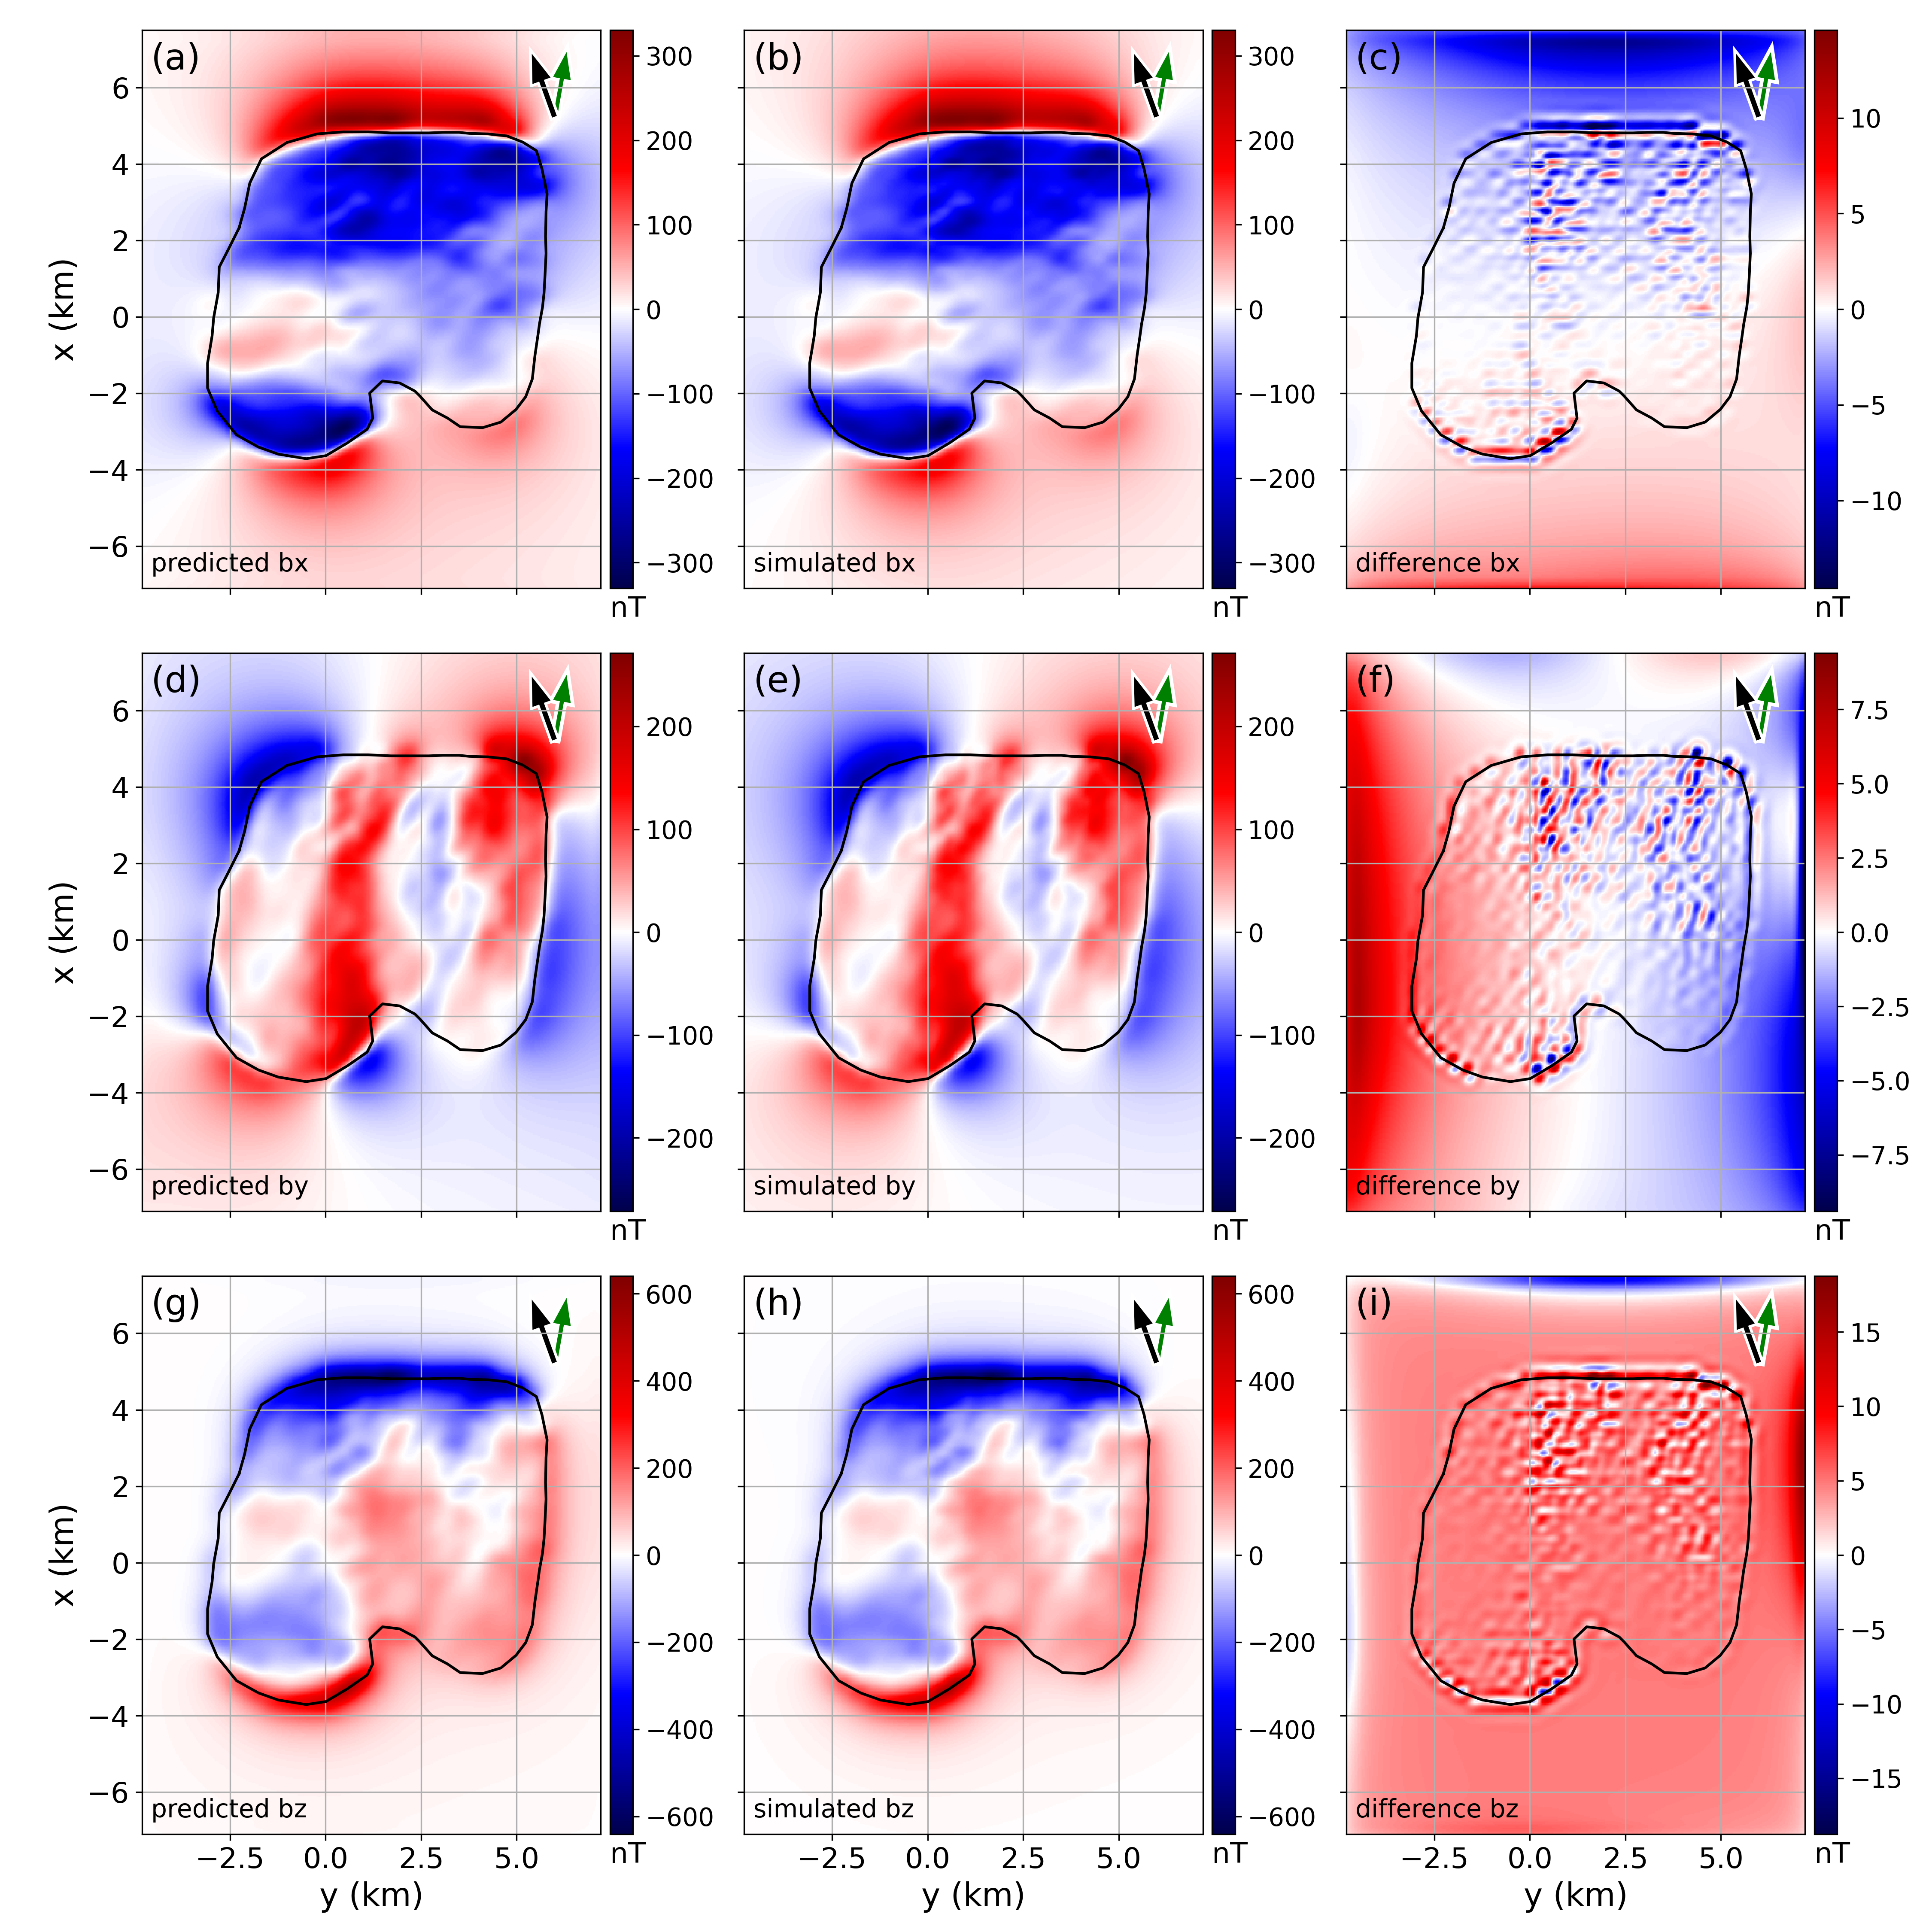
\includegraphics[width=0.8\textwidth]{Figure_S19.png}
	\caption{%
		Comparison between the simulated fields and those predicted by the estimated equivalent layer shown in Figure \mainref{fig:Figure4}i.
	}
	\label{S-fig:FigureS19}
\end{figure}

\begin{figure}[h]
	\centering
	\noindent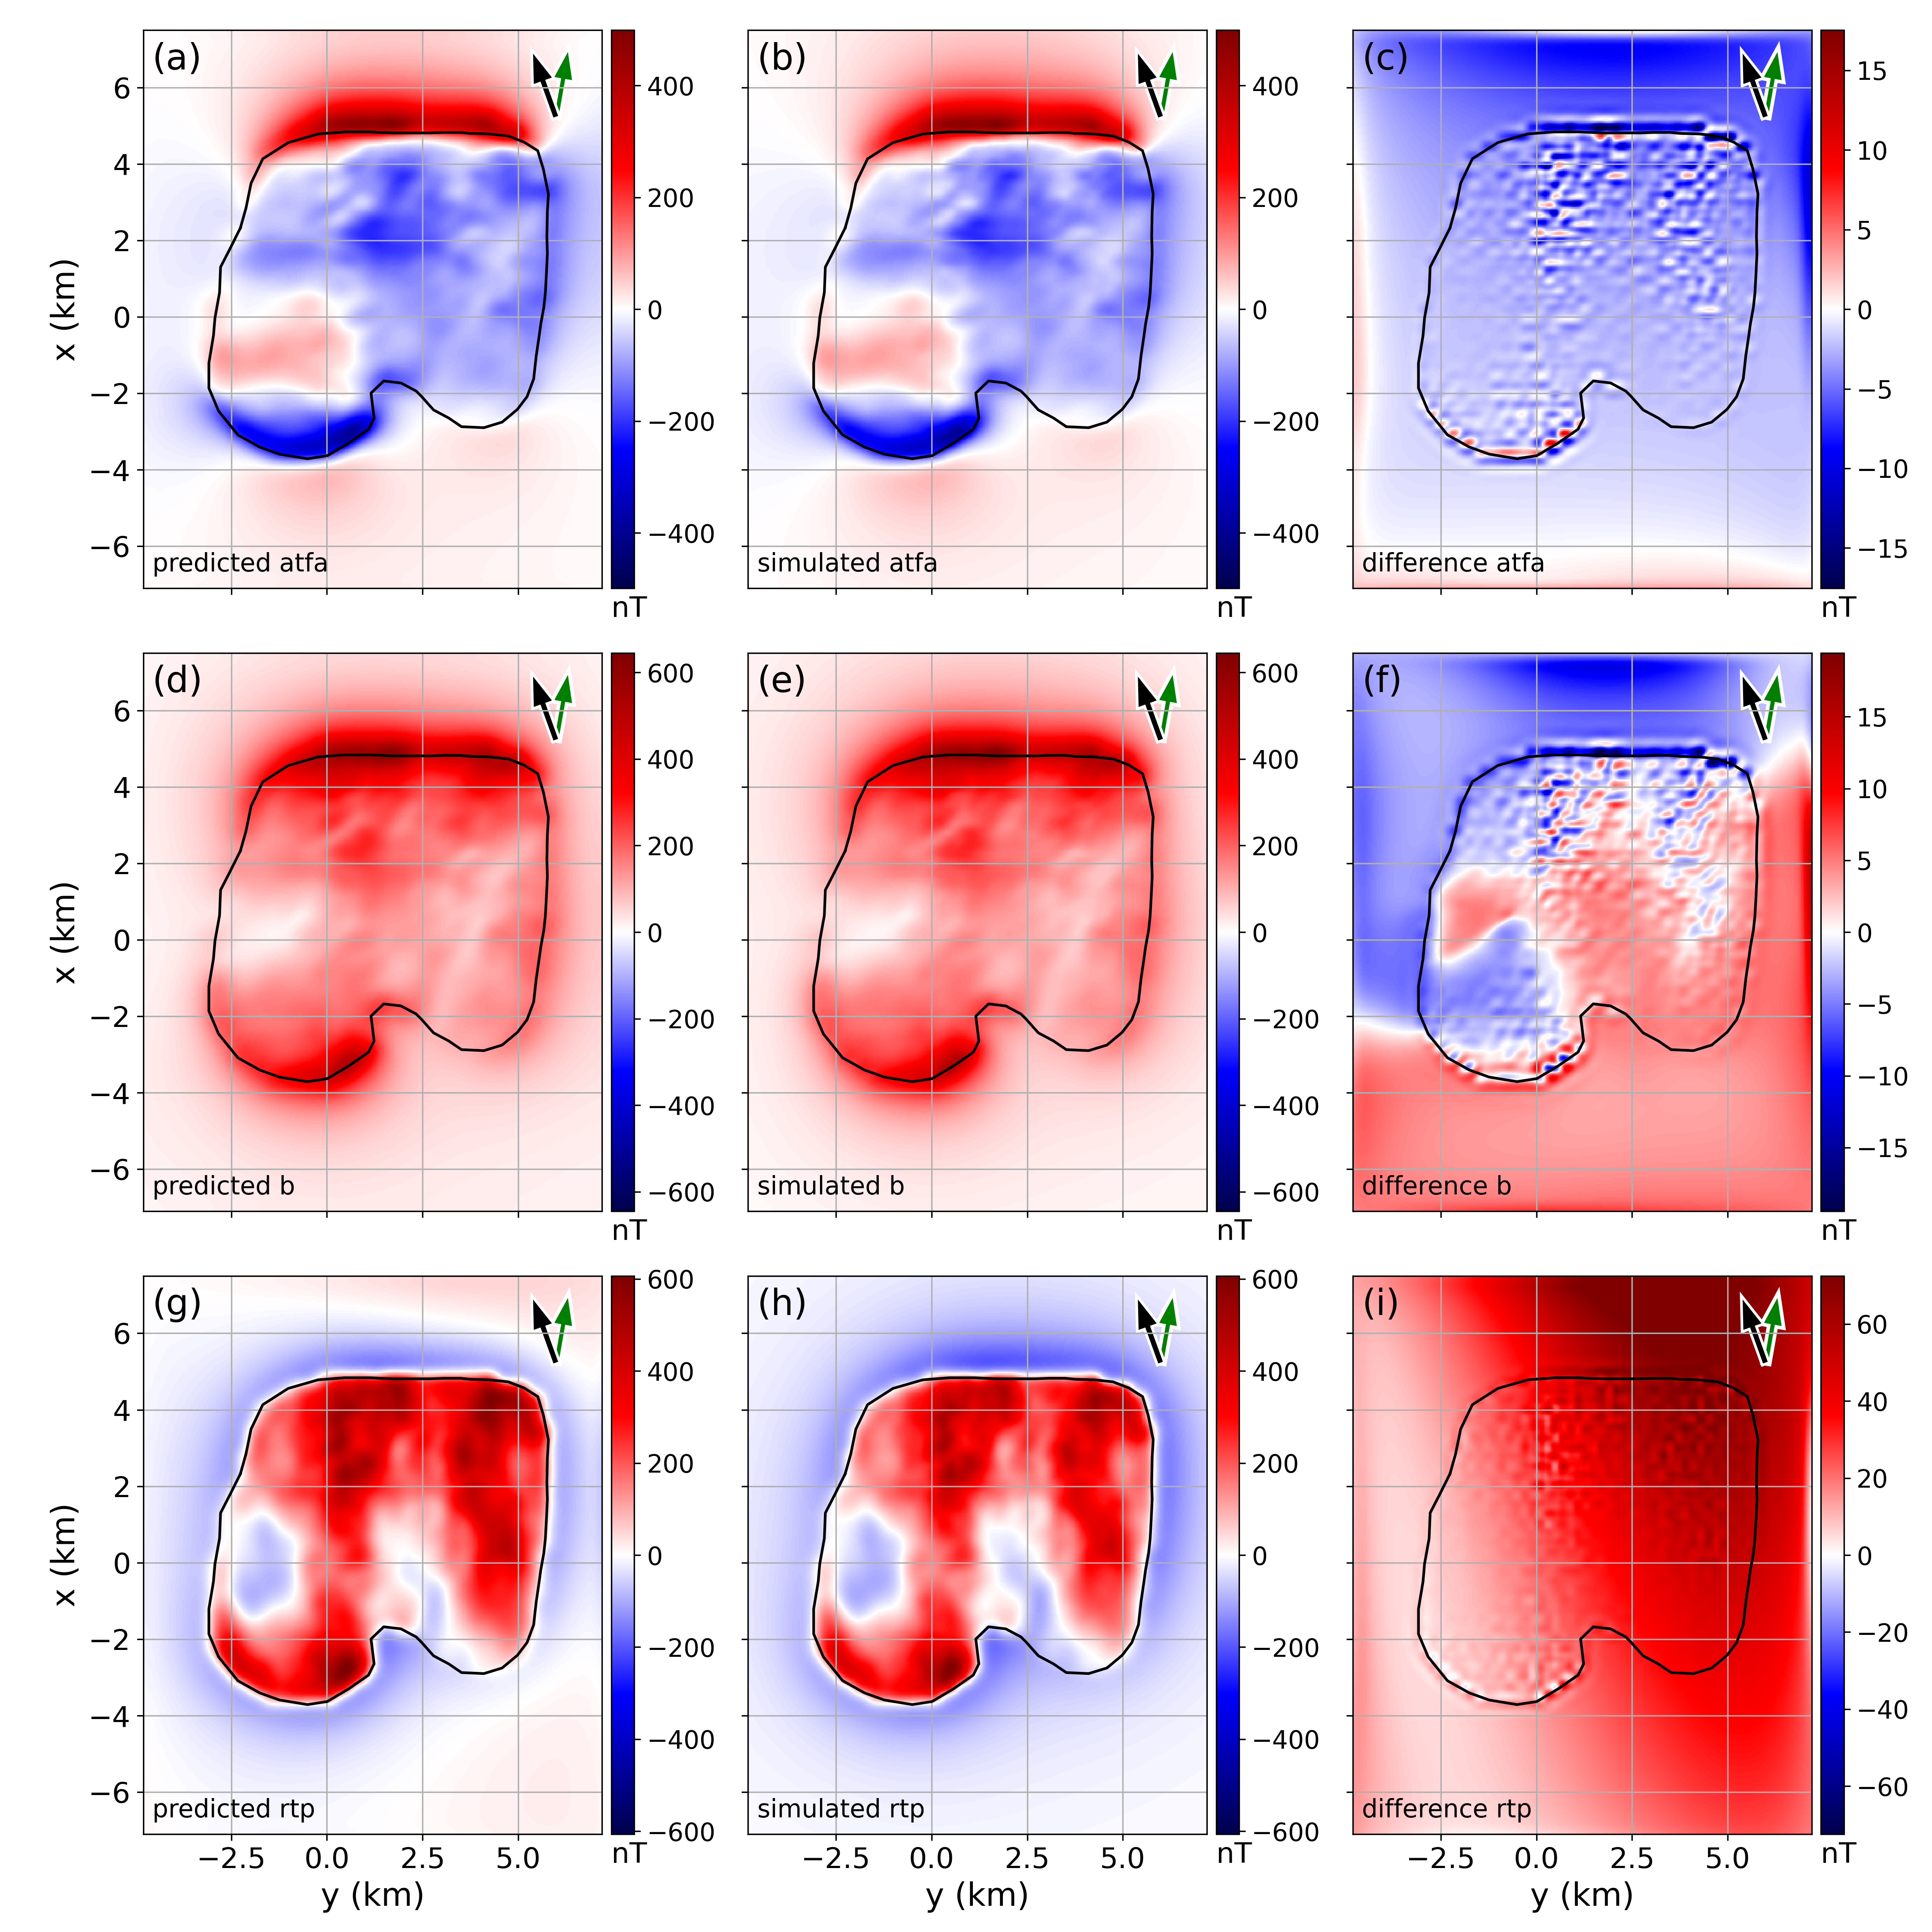
\includegraphics[width=0.8\textwidth]{Figure_S20.png}
	\caption{%
		Comparison between the simulated fields and those predicted by the estimated equivalent layer shown in Figure \mainref{fig:Figure4}i.
	}
	\label{S-fig:FigureS20}
\end{figure}

\clearpage

\section{Declarations}

%Some journals require declarations to be submitted in a standardised format. Please check the Instructions for Authors of the journal to which you are submitting to see if you need to complete this section. If yes, your manuscript must contain the following sections under the heading `Declarations':

\begin{itemize}
	%\item Funding
	\item Conflict of interest/Competing interests: The authors declare no conflict of interest.
	%\item Ethics approval and consent to participate: Not applicable.
	%\item Consent for publication
	%\item Data availability: Not applicable.
	%\item Materials availability: Not applicable.
	\item Code availability: The Python source code used to produce all results and figures presented in this study is
	available at Zenodo \citep{dataset} under the MIT open-source license. This research made use of the following open-source scientific software: 
	NumPy \citep{numpy} and SciPy \citep{scipy} for numerical computing and linear algebra, Matplotlib \citep{matplotlib} and Vedo \citep{vedo} for 
	visualization, and gravmag \citep{gravmag} for potential field data processing and modeling. \textbf{The Dataset in \cite{dataset} will be made freely 
		available at Zenodo upon publication. During the review process, we opted for sending the code directly for the editors and reviewers via submission 
		system}.
	%\item Author contribution
\end{itemize}

\backmatter

%\bmhead{Supplementary information}
%
%If your article has accompanying supplementary file/s please state so here. 
%
%Authors reporting data from electrophoretic gels and blots should supply the full unprocessed scans for key as part of their Supplementary information. This may be requested by the editorial team/s if it is missing.
%
%Please refer to Journal-level guidance for any specific requirements.

%\bmhead{Acknowledgements}
%This study was financed by the Brazilian agencies Funda{\c c}{\~ a}o Carlos Chagas Filho de Amparo {\` a} Pesquisa do Estado do Rio de Janeiro (FAPERJ) 
%(grant ids E-26 202.729/2018 and 26/202.582/2019) and Conselho Nacional de Desenvolvimento Cient{\' i}fico e Tecnol{\' o}gico (CNPq) (grant ids 315768/2020-7 and 309624/2021-5). The authors thank the editors and reviewers who contributed to this work.

%\noindent
%If any of the sections are not relevant to your manuscript, please include the heading and write `Not applicable' for that section. 


%\begin{appendices}

%\section{Section title of first appendix}\label{secA1}
%
%An appendix contains supplementary information that is not an essential part of the text itself but which may be helpful in providing a more comprehensive understanding of the research problem or it is information that is too cumbersome to be included in the body of the paper.

%%=============================================%%
%% For submissions to Nature Portfolio Journals %%
%% please use the heading ``Extended Data''.   %%
%%=============================================%%

%%=============================================================%%
%% Sample for another appendix section			       %%
%%=============================================================%%

%% \section{Example of another appendix section}\label{secA2}%
%% Appendices may be used for helpful, supporting or essential material that would otherwise 
%% clutter, break up or be distracting to the text. Appendices can consist of sections, figures, 
%% tables and equations etc.

%\end{appendices}

%%===========================================================================================%%
%% If you are submitting to one of the Nature Portfolio journals, using the eJP submission   %%
%% system, please include the references within the manuscript file itself. You may do this  %%
%% by copying the reference list from your .bbl file, paste it into the main manuscript .tex %%
%% file, and delete the associated \verb+\bibliography+ commands.                            %%
%%===========================================================================================%%

\bibliography{references}% common bib file
%% if required, the content of .bbl file can be included here once bbl is generated
%%\input sn-article.bbl

\end{document}
